
    \documentclass{article}
    \usepackage[a4paper, left=1cm, right=1cm, top=2cm, bottom=2cm]{geometry}
    \usepackage{hyperref} % für anklickbare Bezüge 
    \usepackage{tikz} % für MO-Schemata
    \usepackage{amsmath}
    \usepackage{physics}
    \usepackage{float} % to anchor tables 
    
    \allowdisplaybreaks

    \setlength{\parindent}{0pt}
    \hypersetup{colorlinks=true, linkcolor=black, citecolor=black}% damit Referenzen nicht in PDF umklammert

    \begin{document}
    \pagestyle{empty}
    \tableofcontents 
    \newpage 
    \section{Orbitals And Their Symmetry}%Orbitale und deren Symmetrie 

%\includegraphics[scale=0.125]{img/DimerZOrbitalordnung-C6H5Cl-C2h-gesamt-MO-beiWW.pdf}
\vspace{2cm}
We use the following ordering of orbitals here (assuming degeneracy of LUMOs and HOMOs): 

$$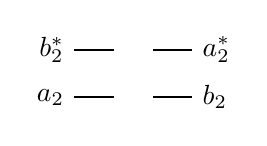
\begin{tikzpicture}[baseline={(current bounding box.center)}]
% lower MOs:
\draw[thick] (0,-0.6) -- (0.5,-0.6)node[pos=0, left] {$a_2$}
;;\draw[thick] (1,-0.6) -- (1.5,-0.6)node[pos=1, right] {$b_2$}
;;
% upper MOs:
\draw[thick] (0,0) -- (0.5,0)node[pos=0, left] {$b_2^{*}$}
;;\draw[thick] (1,0) -- (1.5,0)node[pos=1, right] {$a_2^{*}$}
;;
\end{tikzpicture}$$
In the following, we will leave out the explicit labeling by orbital symmetry. Each monomer will simply be written as:

$$\begin{tikzpicture}[baseline={(current bounding box.center)}]
% lower MOs:
\draw[thick] (0,-0.6) -- (0.5,-0.6)%node[pos=0, left] {$a_2$}
;;\draw[thick] (1,-0.6) -- (1.5,-0.6)%node[pos=1, right] {$b_2$}
;;
% upper MOs:
\draw[thick] (0,0) -- (0.5,0)%node[pos=0, left] {$b_2^{*}$}
;;\draw[thick] (1,0) -- (1.5,0)%node[pos=1, right] {$a_2^{*}$}
;;
\end{tikzpicture}$$
where the character of the orbital is defined by its position. \\ \\ 


Dimer configurations will be written as their monomer occupations, by writing one monomer to the left and one to the right. The orbital ordering within the group of monomer orbitals follows the above mentioned definition. \\ \\ The transformation of monomer orbitals into dimer orbitals is given by knowing the negative and positive linear combinations of monomer orbitals into dimer orbitals. Transforming this known equation system leads to: 
\begin{subequations}\begin{gather*}
a_2^{*l} = +a_u^{*}+b_g^{*}  \\
b_2^{*l} = +a_g^{*}+b_u^{*}  \\
a_2^{\mathsf{l}} = +a_{u}+b_g  \\
b_2^{\mathsf{l}} = +a_{g}+b_u  \\
a_2^{*r} = +a_u^{*}-b_g^{*}  \\
b_2^{*r} = -a_g^{*}+b_u^{*}  \\
a_2^{\mathsf{r}} = +a_{u}-b_g  \\
b_2^{\mathsf{r}} = -a_{g}+b_u
\end{gather*}\end{subequations}
\newpage

\section{Monomer States and Configurations} 
\[S = 
 \quad + \left(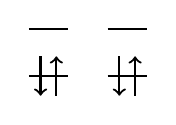
\begin{tikzpicture}[baseline={(current bounding box.center)}]
% lower MOs:
\draw[thick] (0,-0.6) -- (0.5,-0.6)%node[pos=0, left] {$a_2$}
;\draw[->, thick] (0.35, -0.85) -- (0.35, -0.35) ; 
 \draw[<-, thick] (0.15, -0.85) -- (0.15, -0.35) ;\draw[thick] (1,-0.6) -- (1.5,-0.6)%node[pos=1, right] {$b_2$}
;\draw[->, thick] (1.35, -0.85) -- (1.35, -0.35) ; 
 \draw[<-, thick] (1.15, -0.85) -- (1.15, -0.35) ;
% upper MOs:
\draw[thick] (0,0) -- (0.5,0)%node[pos=0, left] {$b_2^{*}$}
;;\draw[thick] (1,0) -- (1.5,0)%node[pos=1, right] {$a_2^{*}$}
;;
\end{tikzpicture}\right) 
 \quad = \left|\underbrace{(b_2^{\mathsf{l}})^{2}(b_2^{*l})^{0}(a_2^{\mathsf{l}})^{2}(a_2^{*l})^{0}}_{a_{g}}\right|\]
\[Q = 
 \quad + \left(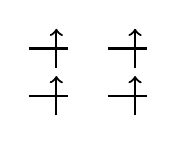
\begin{tikzpicture}[baseline={(current bounding box.center)}]
% lower MOs:
\draw[thick] (0,-0.6) -- (0.5,-0.6)%node[pos=0, left] {$a_2$}
;\draw[->, thick] (0.35, -0.85) -- (0.35, -0.35) ;\draw[thick] (1,-0.6) -- (1.5,-0.6)%node[pos=1, right] {$b_2$}
;\draw[->, thick] (1.35, -0.85) -- (1.35, -0.35) ;
% upper MOs:
\draw[thick] (0,0) -- (0.5,0)%node[pos=0, left] {$b_2^{*}$}
;\draw[->, thick] (0.35, -0.25) -- (0.35, 0.25) ;\draw[thick] (1,0) -- (1.5,0)%node[pos=1, right] {$a_2^{*}$}
;\draw[->, thick] (1.35, -0.25) -- (1.35, 0.25) ;
\end{tikzpicture}\right) 
 \quad = \left|\underbrace{(b_2^{\mathsf{l}})^{1}(b_2^{*l})^{1}(a_2^{\mathsf{l}})^{1}(a_2^{*l})^{1}}_{a_1}\right|\]
\[i^3 a_1 = 
 \quad + \left(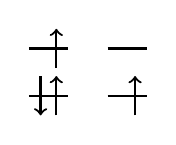
\begin{tikzpicture}[baseline={(current bounding box.center)}]
% lower MOs:
\draw[thick] (0,-0.6) -- (0.5,-0.6)%node[pos=0, left] {$a_2$}
;\draw[->, thick] (0.35, -0.85) -- (0.35, -0.35) ; 
 \draw[<-, thick] (0.15, -0.85) -- (0.15, -0.35) ;\draw[thick] (1,-0.6) -- (1.5,-0.6)%node[pos=1, right] {$b_2$}
;\draw[->, thick] (1.35, -0.85) -- (1.35, -0.35) ;
% upper MOs:
\draw[thick] (0,0) -- (0.5,0)%node[pos=0, left] {$b_2^{*}$}
;\draw[->, thick] (0.35, -0.25) -- (0.35, 0.25) ;\draw[thick] (1,0) -- (1.5,0)%node[pos=1, right] {$a_2^{*}$}
;;
\end{tikzpicture}\right) 
- \left(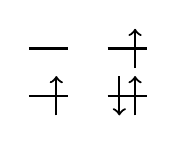
\begin{tikzpicture}[baseline={(current bounding box.center)}]
% lower MOs:
\draw[thick] (0,-0.6) -- (0.5,-0.6)%node[pos=0, left] {$a_2$}
;\draw[->, thick] (0.35, -0.85) -- (0.35, -0.35) ;\draw[thick] (1,-0.6) -- (1.5,-0.6)%node[pos=1, right] {$b_2$}
;\draw[->, thick] (1.35, -0.85) -- (1.35, -0.35) ; 
 \draw[<-, thick] (1.15, -0.85) -- (1.15, -0.35) ;
% upper MOs:
\draw[thick] (0,0) -- (0.5,0)%node[pos=0, left] {$b_2^{*}$}
;;\draw[thick] (1,0) -- (1.5,0)%node[pos=1, right] {$a_2^{*}$}
;\draw[->, thick] (1.35, -0.25) -- (1.35, 0.25) ;
\end{tikzpicture}\right) 
 \quad = \left|\underbrace{(b_2^{\mathsf{l}})^{1}(b_2^{*l})^{1}(a_2^{\mathsf{l}})^{2}(a_2^{*l})^{0}}_{a_1}\right| - \left|\underbrace{(b_2^{\mathsf{l}})^{2}(b_2^{*l})^{0}(a_2^{\mathsf{l}})^{1}(a_2^{*l})^{1}}_{a_1}\right|\]
\[e^3 a_1 = 
 \quad + \left(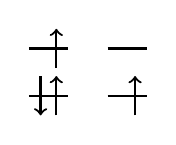
\begin{tikzpicture}[baseline={(current bounding box.center)}]
% lower MOs:
\draw[thick] (0,-0.6) -- (0.5,-0.6)%node[pos=0, left] {$a_2$}
;\draw[->, thick] (0.35, -0.85) -- (0.35, -0.35) ; 
 \draw[<-, thick] (0.15, -0.85) -- (0.15, -0.35) ;\draw[thick] (1,-0.6) -- (1.5,-0.6)%node[pos=1, right] {$b_2$}
;\draw[->, thick] (1.35, -0.85) -- (1.35, -0.35) ;
% upper MOs:
\draw[thick] (0,0) -- (0.5,0)%node[pos=0, left] {$b_2^{*}$}
;\draw[->, thick] (0.35, -0.25) -- (0.35, 0.25) ;\draw[thick] (1,0) -- (1.5,0)%node[pos=1, right] {$a_2^{*}$}
;;
\end{tikzpicture}\right) 
+ \left(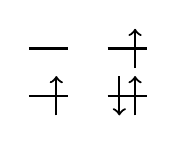
\begin{tikzpicture}[baseline={(current bounding box.center)}]
% lower MOs:
\draw[thick] (0,-0.6) -- (0.5,-0.6)%node[pos=0, left] {$a_2$}
;\draw[->, thick] (0.35, -0.85) -- (0.35, -0.35) ;\draw[thick] (1,-0.6) -- (1.5,-0.6)%node[pos=1, right] {$b_2$}
;\draw[->, thick] (1.35, -0.85) -- (1.35, -0.35) ; 
 \draw[<-, thick] (1.15, -0.85) -- (1.15, -0.35) ;
% upper MOs:
\draw[thick] (0,0) -- (0.5,0)%node[pos=0, left] {$b_2^{*}$}
;;\draw[thick] (1,0) -- (1.5,0)%node[pos=1, right] {$a_2^{*}$}
;\draw[->, thick] (1.35, -0.25) -- (1.35, 0.25) ;
\end{tikzpicture}\right) 
 \quad = \left|\underbrace{(b_2^{\mathsf{l}})^{1}(b_2^{*l})^{1}(a_2^{\mathsf{l}})^{2}(a_2^{*l})^{0}}_{a_1}\right| + \left|\underbrace{(b_2^{\mathsf{l}})^{2}(b_2^{*l})^{0}(a_2^{\mathsf{l}})^{1}(a_2^{*l})^{1}}_{a_1}\right|\]
\[i^3 b_{1} = 
 \quad + \left(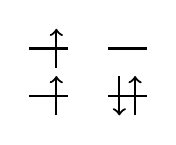
\begin{tikzpicture}[baseline={(current bounding box.center)}]
% lower MOs:
\draw[thick] (0,-0.6) -- (0.5,-0.6)%node[pos=0, left] {$a_2$}
;\draw[->, thick] (0.35, -0.85) -- (0.35, -0.35) ;\draw[thick] (1,-0.6) -- (1.5,-0.6)%node[pos=1, right] {$b_2$}
;\draw[->, thick] (1.35, -0.85) -- (1.35, -0.35) ; 
 \draw[<-, thick] (1.15, -0.85) -- (1.15, -0.35) ;
% upper MOs:
\draw[thick] (0,0) -- (0.5,0)%node[pos=0, left] {$b_2^{*}$}
;\draw[->, thick] (0.35, -0.25) -- (0.35, 0.25) ;\draw[thick] (1,0) -- (1.5,0)%node[pos=1, right] {$a_2^{*}$}
;;
\end{tikzpicture}\right) 
- \left(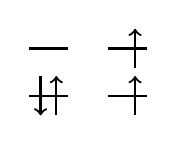
\begin{tikzpicture}[baseline={(current bounding box.center)}]
% lower MOs:
\draw[thick] (0,-0.6) -- (0.5,-0.6)%node[pos=0, left] {$a_2$}
;\draw[->, thick] (0.35, -0.85) -- (0.35, -0.35) ; 
 \draw[<-, thick] (0.15, -0.85) -- (0.15, -0.35) ;\draw[thick] (1,-0.6) -- (1.5,-0.6)%node[pos=1, right] {$b_2$}
;\draw[->, thick] (1.35, -0.85) -- (1.35, -0.35) ;
% upper MOs:
\draw[thick] (0,0) -- (0.5,0)%node[pos=0, left] {$b_2^{*}$}
;;\draw[thick] (1,0) -- (1.5,0)%node[pos=1, right] {$a_2^{*}$}
;\draw[->, thick] (1.35, -0.25) -- (1.35, 0.25) ;
\end{tikzpicture}\right) 
 \quad = \left|\underbrace{(b_2^{\mathsf{l}})^{2}(b_2^{*l})^{1}(a_2^{\mathsf{l}})^{1}(a_2^{*l})^{0}}_{b_1}\right| - \left|\underbrace{(b_2^{\mathsf{l}})^{1}(b_2^{*l})^{0}(a_2^{\mathsf{l}})^{2}(a_2^{*l})^{1}}_{b_1}\right|\]
\[e^3 b_{1} = 
 \quad + \left(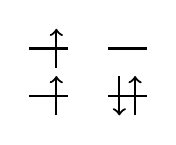
\begin{tikzpicture}[baseline={(current bounding box.center)}]
% lower MOs:
\draw[thick] (0,-0.6) -- (0.5,-0.6)%node[pos=0, left] {$a_2$}
;\draw[->, thick] (0.35, -0.85) -- (0.35, -0.35) ;\draw[thick] (1,-0.6) -- (1.5,-0.6)%node[pos=1, right] {$b_2$}
;\draw[->, thick] (1.35, -0.85) -- (1.35, -0.35) ; 
 \draw[<-, thick] (1.15, -0.85) -- (1.15, -0.35) ;
% upper MOs:
\draw[thick] (0,0) -- (0.5,0)%node[pos=0, left] {$b_2^{*}$}
;\draw[->, thick] (0.35, -0.25) -- (0.35, 0.25) ;\draw[thick] (1,0) -- (1.5,0)%node[pos=1, right] {$a_2^{*}$}
;;
\end{tikzpicture}\right) 
+ \left(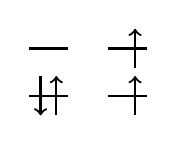
\begin{tikzpicture}[baseline={(current bounding box.center)}]
% lower MOs:
\draw[thick] (0,-0.6) -- (0.5,-0.6)%node[pos=0, left] {$a_2$}
;\draw[->, thick] (0.35, -0.85) -- (0.35, -0.35) ; 
 \draw[<-, thick] (0.15, -0.85) -- (0.15, -0.35) ;\draw[thick] (1,-0.6) -- (1.5,-0.6)%node[pos=1, right] {$b_2$}
;\draw[->, thick] (1.35, -0.85) -- (1.35, -0.35) ;
% upper MOs:
\draw[thick] (0,0) -- (0.5,0)%node[pos=0, left] {$b_2^{*}$}
;;\draw[thick] (1,0) -- (1.5,0)%node[pos=1, right] {$a_2^{*}$}
;\draw[->, thick] (1.35, -0.25) -- (1.35, 0.25) ;
\end{tikzpicture}\right) 
 \quad = \left|\underbrace{(b_2^{\mathsf{l}})^{2}(b_2^{*l})^{1}(a_2^{\mathsf{l}})^{1}(a_2^{*l})^{0}}_{b_1}\right| + \left|\underbrace{(b_2^{\mathsf{l}})^{1}(b_2^{*l})^{0}(a_2^{\mathsf{l}})^{2}(a_2^{*l})^{1}}_{b_1}\right|\]
\newpage

\section{Linear Combinations} 

\subsection{\boldmath $S \otimes Q + Q \otimes S$}
\[S \otimes Q + Q \otimes S\]
\[+ \left(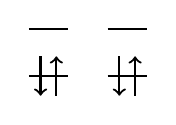
\begin{tikzpicture}[baseline={(current bounding box.center)}]
% lower MOs:
\draw[thick] (0,-0.6) -- (0.5,-0.6)%node[pos=0, left] {$a_2$}
;\draw[->, thick] (0.35, -0.85) -- (0.35, -0.35) ; 
 \draw[<-, thick] (0.15, -0.85) -- (0.15, -0.35) ;\draw[thick] (1,-0.6) -- (1.5,-0.6)%node[pos=1, right] {$b_2$}
;\draw[->, thick] (1.35, -0.85) -- (1.35, -0.35) ; 
 \draw[<-, thick] (1.15, -0.85) -- (1.15, -0.35) ;
% upper MOs:
\draw[thick] (0,0) -- (0.5,0)%node[pos=0, left] {$b_2^{*}$}
;;\draw[thick] (1,0) -- (1.5,0)%node[pos=1, right] {$a_2^{*}$}
;;
\end{tikzpicture}
\quad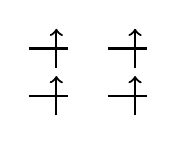
\begin{tikzpicture}[baseline={(current bounding box.center)}]
% lower MOs:
\draw[thick] (0,-0.6) -- (0.5,-0.6)%node[pos=0, left] {$a_2$}
;\draw[->, thick] (0.35, -0.85) -- (0.35, -0.35) ;\draw[thick] (1,-0.6) -- (1.5,-0.6)%node[pos=1, right] {$b_2$}
;\draw[->, thick] (1.35, -0.85) -- (1.35, -0.35) ;
% upper MOs:
\draw[thick] (0,0) -- (0.5,0)%node[pos=0, left] {$b_2^{*}$}
;\draw[->, thick] (0.35, -0.25) -- (0.35, 0.25) ;\draw[thick] (1,0) -- (1.5,0)%node[pos=1, right] {$a_2^{*}$}
;\draw[->, thick] (1.35, -0.25) -- (1.35, 0.25) ;
\end{tikzpicture}\right) 
 + \left(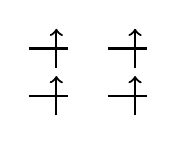
\begin{tikzpicture}[baseline={(current bounding box.center)}]
% lower MOs:
\draw[thick] (0,-0.6) -- (0.5,-0.6)%node[pos=0, left] {$a_2$}
;\draw[->, thick] (0.35, -0.85) -- (0.35, -0.35) ;\draw[thick] (1,-0.6) -- (1.5,-0.6)%node[pos=1, right] {$b_2$}
;\draw[->, thick] (1.35, -0.85) -- (1.35, -0.35) ;
% upper MOs:
\draw[thick] (0,0) -- (0.5,0)%node[pos=0, left] {$b_2^{*}$}
;\draw[->, thick] (0.35, -0.25) -- (0.35, 0.25) ;\draw[thick] (1,0) -- (1.5,0)%node[pos=1, right] {$a_2^{*}$}
;\draw[->, thick] (1.35, -0.25) -- (1.35, 0.25) ;
\end{tikzpicture}
\quad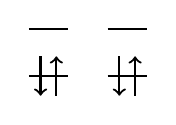
\begin{tikzpicture}[baseline={(current bounding box.center)}]
% lower MOs:
\draw[thick] (0,-0.6) -- (0.5,-0.6)%node[pos=0, left] {$a_2$}
;\draw[->, thick] (0.35, -0.85) -- (0.35, -0.35) ; 
 \draw[<-, thick] (0.15, -0.85) -- (0.15, -0.35) ;\draw[thick] (1,-0.6) -- (1.5,-0.6)%node[pos=1, right] {$b_2$}
;\draw[->, thick] (1.35, -0.85) -- (1.35, -0.35) ; 
 \draw[<-, thick] (1.15, -0.85) -- (1.15, -0.35) ;
% upper MOs:
\draw[thick] (0,0) -- (0.5,0)%node[pos=0, left] {$b_2^{*}$}
;;\draw[thick] (1,0) -- (1.5,0)%node[pos=1, right] {$a_2^{*}$}
;;
\end{tikzpicture}\right) 
\]
monomer ci vectors:
$$\begin{array}{c}
+\left|\underbrace{(b_2^{\mathsf{l}})^{2}(b_2^{*l})^{0}(a_2^{\mathsf{l}})^{2}(a_2^{*l})^{0}}_{a_{g}^{\mathsf{l}}}\right| \otimes{} \left|\underbrace{(b_2^{\mathsf{r}})^{1}(b_2^{*r})^{1}(a_2^{\mathsf{r}})^{1}(a_2^{*r})^{1}}_{a_1^{\mathsf{r}}}\right| +\left|\underbrace{(b_2^{\mathsf{l}})^{1}(b_2^{*l})^{1}(a_2^{\mathsf{l}})^{1}(a_2^{*l})^{1}}_{a_1^{\mathsf{l}}}\right| \otimes{} \left|\underbrace{(b_2^{\mathsf{r}})^{2}(b_2^{*r})^{0}(a_2^{\mathsf{r}})^{2}(a_2^{*r})^{0}}_{a_{g}^{\mathsf{r}}}\right|
\end{array}$$substitution by dimer orbitals:
$$+\left|\underbrace{(+a_{g}+b_u)^{2}(+a_g^{*}+b_u^{*})^{0}(+a_{u}+b_g)^{2}(+a_u^{*}+b_g^{*})^{0}}_{a_{g}^{\mathsf{l}}}\right| \otimes{} \left|\underbrace{(-a_{g}+b_u)^{1}(-a_g^{*}+b_u^{*})^{1}(+a_{u}-b_g)^{1}(+a_u^{*}-b_g^{*})^{1}}_{a_1^{\mathsf{r}}}\right| + \hdots $$(multiplied out and summed up) dimer ci vectors:

\begin{multline*}\begin{array}{c}
-2 \cdot \left|\underbrace{(a_{g})^{2}(b_u)^{1}(a_{u})^{2}(b_g)^{1}(a_g^{*})^{0}(b_u^{*})^{1}(a_u^{*})^{0}(b_g^{*})^{1}}_{a_{g}}\right| -2 \cdot \left|\underbrace{(a_{g})^{2}(b_u)^{1}(a_{u})^{1}(b_g)^{2}(a_g^{*})^{0}(b_u^{*})^{1}(a_u^{*})^{1}(b_g^{*})^{0}}_{a_{g}}\right| \\[0.5cm] -2 \cdot \left|\underbrace{(a_{g})^{2}(b_u)^{1}(a_{u})^{2}(b_g)^{1}(a_g^{*})^{1}(b_u^{*})^{0}(a_u^{*})^{1}(b_g^{*})^{0}}_{a_{g}}\right| -2 \cdot \left|\underbrace{(a_{g})^{2}(b_u)^{1}(a_{u})^{1}(b_g)^{2}(a_g^{*})^{1}(b_u^{*})^{0}(a_u^{*})^{0}(b_g^{*})^{1}}_{a_{g}}\right| \\[0.5cm] -2 \cdot \left|\underbrace{(a_{g})^{1}(b_u)^{2}(a_{u})^{2}(b_g)^{1}(a_g^{*})^{0}(b_u^{*})^{1}(a_u^{*})^{1}(b_g^{*})^{0}}_{a_{g}}\right| -2 \cdot \left|\underbrace{(a_{g})^{1}(b_u)^{2}(a_{u})^{1}(b_g)^{2}(a_g^{*})^{0}(b_u^{*})^{1}(a_u^{*})^{0}(b_g^{*})^{1}}_{a_{g}}\right| \\[0.5cm] -2 \cdot \left|\underbrace{(a_{g})^{1}(b_u)^{2}(a_{u})^{2}(b_g)^{1}(a_g^{*})^{1}(b_u^{*})^{0}(a_u^{*})^{0}(b_g^{*})^{1}}_{a_{g}}\right| -2 \cdot \left|\underbrace{(a_{g})^{1}(b_u)^{2}(a_{u})^{1}(b_g)^{2}(a_g^{*})^{1}(b_u^{*})^{0}(a_u^{*})^{1}(b_g^{*})^{0}}_{a_{g}}\right|
\end{array}\end{multline*}


\vspace{0.5cm}

\newpage

\subsection{\boldmath $S \otimes Q - Q \otimes S$}
\[S \otimes Q - Q \otimes S\]
\[+ \left(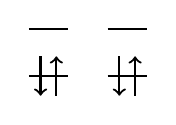
\begin{tikzpicture}[baseline={(current bounding box.center)}]
% lower MOs:
\draw[thick] (0,-0.6) -- (0.5,-0.6)%node[pos=0, left] {$a_2$}
;\draw[->, thick] (0.35, -0.85) -- (0.35, -0.35) ; 
 \draw[<-, thick] (0.15, -0.85) -- (0.15, -0.35) ;\draw[thick] (1,-0.6) -- (1.5,-0.6)%node[pos=1, right] {$b_2$}
;\draw[->, thick] (1.35, -0.85) -- (1.35, -0.35) ; 
 \draw[<-, thick] (1.15, -0.85) -- (1.15, -0.35) ;
% upper MOs:
\draw[thick] (0,0) -- (0.5,0)%node[pos=0, left] {$b_2^{*}$}
;;\draw[thick] (1,0) -- (1.5,0)%node[pos=1, right] {$a_2^{*}$}
;;
\end{tikzpicture}
\quad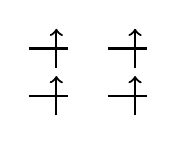
\begin{tikzpicture}[baseline={(current bounding box.center)}]
% lower MOs:
\draw[thick] (0,-0.6) -- (0.5,-0.6)%node[pos=0, left] {$a_2$}
;\draw[->, thick] (0.35, -0.85) -- (0.35, -0.35) ;\draw[thick] (1,-0.6) -- (1.5,-0.6)%node[pos=1, right] {$b_2$}
;\draw[->, thick] (1.35, -0.85) -- (1.35, -0.35) ;
% upper MOs:
\draw[thick] (0,0) -- (0.5,0)%node[pos=0, left] {$b_2^{*}$}
;\draw[->, thick] (0.35, -0.25) -- (0.35, 0.25) ;\draw[thick] (1,0) -- (1.5,0)%node[pos=1, right] {$a_2^{*}$}
;\draw[->, thick] (1.35, -0.25) -- (1.35, 0.25) ;
\end{tikzpicture}\right) 
 - \left(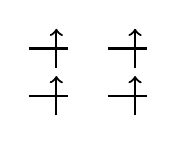
\begin{tikzpicture}[baseline={(current bounding box.center)}]
% lower MOs:
\draw[thick] (0,-0.6) -- (0.5,-0.6)%node[pos=0, left] {$a_2$}
;\draw[->, thick] (0.35, -0.85) -- (0.35, -0.35) ;\draw[thick] (1,-0.6) -- (1.5,-0.6)%node[pos=1, right] {$b_2$}
;\draw[->, thick] (1.35, -0.85) -- (1.35, -0.35) ;
% upper MOs:
\draw[thick] (0,0) -- (0.5,0)%node[pos=0, left] {$b_2^{*}$}
;\draw[->, thick] (0.35, -0.25) -- (0.35, 0.25) ;\draw[thick] (1,0) -- (1.5,0)%node[pos=1, right] {$a_2^{*}$}
;\draw[->, thick] (1.35, -0.25) -- (1.35, 0.25) ;
\end{tikzpicture}
\quad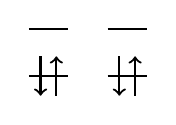
\begin{tikzpicture}[baseline={(current bounding box.center)}]
% lower MOs:
\draw[thick] (0,-0.6) -- (0.5,-0.6)%node[pos=0, left] {$a_2$}
;\draw[->, thick] (0.35, -0.85) -- (0.35, -0.35) ; 
 \draw[<-, thick] (0.15, -0.85) -- (0.15, -0.35) ;\draw[thick] (1,-0.6) -- (1.5,-0.6)%node[pos=1, right] {$b_2$}
;\draw[->, thick] (1.35, -0.85) -- (1.35, -0.35) ; 
 \draw[<-, thick] (1.15, -0.85) -- (1.15, -0.35) ;
% upper MOs:
\draw[thick] (0,0) -- (0.5,0)%node[pos=0, left] {$b_2^{*}$}
;;\draw[thick] (1,0) -- (1.5,0)%node[pos=1, right] {$a_2^{*}$}
;;
\end{tikzpicture}\right) 
\]
monomer ci vectors:
$$\begin{array}{c}
+\left|\underbrace{(b_2^{\mathsf{l}})^{2}(b_2^{*l})^{0}(a_2^{\mathsf{l}})^{2}(a_2^{*l})^{0}}_{a_{g}^{\mathsf{l}}}\right| \otimes{} \left|\underbrace{(b_2^{\mathsf{r}})^{1}(b_2^{*r})^{1}(a_2^{\mathsf{r}})^{1}(a_2^{*r})^{1}}_{a_1^{\mathsf{r}}}\right| -\left|\underbrace{(b_2^{\mathsf{l}})^{1}(b_2^{*l})^{1}(a_2^{\mathsf{l}})^{1}(a_2^{*l})^{1}}_{a_1^{\mathsf{l}}}\right| \otimes{} \left|\underbrace{(b_2^{\mathsf{r}})^{2}(b_2^{*r})^{0}(a_2^{\mathsf{r}})^{2}(a_2^{*r})^{0}}_{a_{g}^{\mathsf{r}}}\right|
\end{array}$$substitution by dimer orbitals:
$$+\left|\underbrace{(+a_{g}+b_u)^{2}(+a_g^{*}+b_u^{*})^{0}(+a_{u}+b_g)^{2}(+a_u^{*}+b_g^{*})^{0}}_{a_{g}^{\mathsf{l}}}\right| \otimes{} \left|\underbrace{(-a_{g}+b_u)^{1}(-a_g^{*}+b_u^{*})^{1}(+a_{u}-b_g)^{1}(+a_u^{*}-b_g^{*})^{1}}_{a_1^{\mathsf{r}}}\right| + \hdots $$(multiplied out and summed up) dimer ci vectors:

\begin{multline*}\begin{array}{c}
+2 \cdot \left|\underbrace{(a_{g})^{2}(b_u)^{1}(a_{u})^{2}(b_g)^{1}(a_g^{*})^{0}(b_u^{*})^{1}(a_u^{*})^{1}(b_g^{*})^{0}}_{b_u}\right| +2 \cdot \left|\underbrace{(a_{g})^{2}(b_u)^{1}(a_{u})^{1}(b_g)^{2}(a_g^{*})^{0}(b_u^{*})^{1}(a_u^{*})^{0}(b_g^{*})^{1}}_{b_u}\right| \\[0.5cm] +2 \cdot \left|\underbrace{(a_{g})^{2}(b_u)^{1}(a_{u})^{2}(b_g)^{1}(a_g^{*})^{1}(b_u^{*})^{0}(a_u^{*})^{0}(b_g^{*})^{1}}_{b_u}\right| +2 \cdot \left|\underbrace{(a_{g})^{2}(b_u)^{1}(a_{u})^{1}(b_g)^{2}(a_g^{*})^{1}(b_u^{*})^{0}(a_u^{*})^{1}(b_g^{*})^{0}}_{b_u}\right| \\[0.5cm] +2 \cdot \left|\underbrace{(a_{g})^{1}(b_u)^{2}(a_{u})^{2}(b_g)^{1}(a_g^{*})^{0}(b_u^{*})^{1}(a_u^{*})^{0}(b_g^{*})^{1}}_{b_u}\right| +2 \cdot \left|\underbrace{(a_{g})^{1}(b_u)^{2}(a_{u})^{1}(b_g)^{2}(a_g^{*})^{0}(b_u^{*})^{1}(a_u^{*})^{1}(b_g^{*})^{0}}_{b_u}\right| \\[0.5cm] +2 \cdot \left|\underbrace{(a_{g})^{1}(b_u)^{2}(a_{u})^{2}(b_g)^{1}(a_g^{*})^{1}(b_u^{*})^{0}(a_u^{*})^{1}(b_g^{*})^{0}}_{b_u}\right| +2 \cdot \left|\underbrace{(a_{g})^{1}(b_u)^{2}(a_{u})^{1}(b_g)^{2}(a_g^{*})^{1}(b_u^{*})^{0}(a_u^{*})^{0}(b_g^{*})^{1}}_{b_u}\right|
\end{array}\end{multline*}


\vspace{0.5cm}

\newpage

\subsection{\boldmath $i^3 a_1 \otimes i^3 a_1$}
\[i^3 a_1 \otimes i^3 a_1\]
\[\begin{array}{c}
+ \left(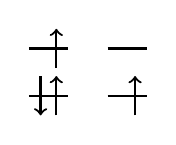
\begin{tikzpicture}[baseline={(current bounding box.center)}]
% lower MOs:
\draw[thick] (0,-0.6) -- (0.5,-0.6)%node[pos=0, left] {$a_2$}
;\draw[->, thick] (0.35, -0.85) -- (0.35, -0.35) ; 
 \draw[<-, thick] (0.15, -0.85) -- (0.15, -0.35) ;\draw[thick] (1,-0.6) -- (1.5,-0.6)%node[pos=1, right] {$b_2$}
;\draw[->, thick] (1.35, -0.85) -- (1.35, -0.35) ;
% upper MOs:
\draw[thick] (0,0) -- (0.5,0)%node[pos=0, left] {$b_2^{*}$}
;\draw[->, thick] (0.35, -0.25) -- (0.35, 0.25) ;\draw[thick] (1,0) -- (1.5,0)%node[pos=1, right] {$a_2^{*}$}
;;
\end{tikzpicture}
\quad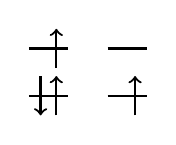
\begin{tikzpicture}[baseline={(current bounding box.center)}]
% lower MOs:
\draw[thick] (0,-0.6) -- (0.5,-0.6)%node[pos=0, left] {$a_2$}
;\draw[->, thick] (0.35, -0.85) -- (0.35, -0.35) ; 
 \draw[<-, thick] (0.15, -0.85) -- (0.15, -0.35) ;\draw[thick] (1,-0.6) -- (1.5,-0.6)%node[pos=1, right] {$b_2$}
;\draw[->, thick] (1.35, -0.85) -- (1.35, -0.35) ;
% upper MOs:
\draw[thick] (0,0) -- (0.5,0)%node[pos=0, left] {$b_2^{*}$}
;\draw[->, thick] (0.35, -0.25) -- (0.35, 0.25) ;\draw[thick] (1,0) -- (1.5,0)%node[pos=1, right] {$a_2^{*}$}
;;
\end{tikzpicture}\right) 
 - \left(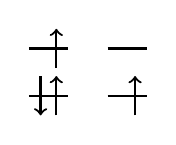
\begin{tikzpicture}[baseline={(current bounding box.center)}]
% lower MOs:
\draw[thick] (0,-0.6) -- (0.5,-0.6)%node[pos=0, left] {$a_2$}
;\draw[->, thick] (0.35, -0.85) -- (0.35, -0.35) ; 
 \draw[<-, thick] (0.15, -0.85) -- (0.15, -0.35) ;\draw[thick] (1,-0.6) -- (1.5,-0.6)%node[pos=1, right] {$b_2$}
;\draw[->, thick] (1.35, -0.85) -- (1.35, -0.35) ;
% upper MOs:
\draw[thick] (0,0) -- (0.5,0)%node[pos=0, left] {$b_2^{*}$}
;\draw[->, thick] (0.35, -0.25) -- (0.35, 0.25) ;\draw[thick] (1,0) -- (1.5,0)%node[pos=1, right] {$a_2^{*}$}
;;
\end{tikzpicture}
\quad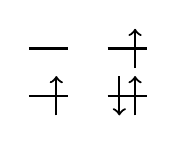
\begin{tikzpicture}[baseline={(current bounding box.center)}]
% lower MOs:
\draw[thick] (0,-0.6) -- (0.5,-0.6)%node[pos=0, left] {$a_2$}
;\draw[->, thick] (0.35, -0.85) -- (0.35, -0.35) ;\draw[thick] (1,-0.6) -- (1.5,-0.6)%node[pos=1, right] {$b_2$}
;\draw[->, thick] (1.35, -0.85) -- (1.35, -0.35) ; 
 \draw[<-, thick] (1.15, -0.85) -- (1.15, -0.35) ;
% upper MOs:
\draw[thick] (0,0) -- (0.5,0)%node[pos=0, left] {$b_2^{*}$}
;;\draw[thick] (1,0) -- (1.5,0)%node[pos=1, right] {$a_2^{*}$}
;\draw[->, thick] (1.35, -0.25) -- (1.35, 0.25) ;
\end{tikzpicture}\right) 
 - \left(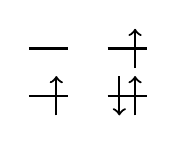
\begin{tikzpicture}[baseline={(current bounding box.center)}]
% lower MOs:
\draw[thick] (0,-0.6) -- (0.5,-0.6)%node[pos=0, left] {$a_2$}
;\draw[->, thick] (0.35, -0.85) -- (0.35, -0.35) ;\draw[thick] (1,-0.6) -- (1.5,-0.6)%node[pos=1, right] {$b_2$}
;\draw[->, thick] (1.35, -0.85) -- (1.35, -0.35) ; 
 \draw[<-, thick] (1.15, -0.85) -- (1.15, -0.35) ;
% upper MOs:
\draw[thick] (0,0) -- (0.5,0)%node[pos=0, left] {$b_2^{*}$}
;;\draw[thick] (1,0) -- (1.5,0)%node[pos=1, right] {$a_2^{*}$}
;\draw[->, thick] (1.35, -0.25) -- (1.35, 0.25) ;
\end{tikzpicture}
\quad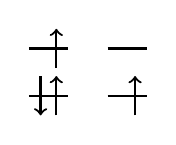
\begin{tikzpicture}[baseline={(current bounding box.center)}]
% lower MOs:
\draw[thick] (0,-0.6) -- (0.5,-0.6)%node[pos=0, left] {$a_2$}
;\draw[->, thick] (0.35, -0.85) -- (0.35, -0.35) ; 
 \draw[<-, thick] (0.15, -0.85) -- (0.15, -0.35) ;\draw[thick] (1,-0.6) -- (1.5,-0.6)%node[pos=1, right] {$b_2$}
;\draw[->, thick] (1.35, -0.85) -- (1.35, -0.35) ;
% upper MOs:
\draw[thick] (0,0) -- (0.5,0)%node[pos=0, left] {$b_2^{*}$}
;\draw[->, thick] (0.35, -0.25) -- (0.35, 0.25) ;\draw[thick] (1,0) -- (1.5,0)%node[pos=1, right] {$a_2^{*}$}
;;
\end{tikzpicture}\right) 
 + \left(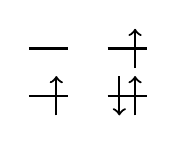
\begin{tikzpicture}[baseline={(current bounding box.center)}]
% lower MOs:
\draw[thick] (0,-0.6) -- (0.5,-0.6)%node[pos=0, left] {$a_2$}
;\draw[->, thick] (0.35, -0.85) -- (0.35, -0.35) ;\draw[thick] (1,-0.6) -- (1.5,-0.6)%node[pos=1, right] {$b_2$}
;\draw[->, thick] (1.35, -0.85) -- (1.35, -0.35) ; 
 \draw[<-, thick] (1.15, -0.85) -- (1.15, -0.35) ;
% upper MOs:
\draw[thick] (0,0) -- (0.5,0)%node[pos=0, left] {$b_2^{*}$}
;;\draw[thick] (1,0) -- (1.5,0)%node[pos=1, right] {$a_2^{*}$}
;\draw[->, thick] (1.35, -0.25) -- (1.35, 0.25) ;
\end{tikzpicture}
\quad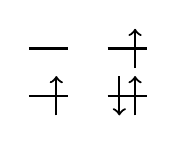
\begin{tikzpicture}[baseline={(current bounding box.center)}]
% lower MOs:
\draw[thick] (0,-0.6) -- (0.5,-0.6)%node[pos=0, left] {$a_2$}
;\draw[->, thick] (0.35, -0.85) -- (0.35, -0.35) ;\draw[thick] (1,-0.6) -- (1.5,-0.6)%node[pos=1, right] {$b_2$}
;\draw[->, thick] (1.35, -0.85) -- (1.35, -0.35) ; 
 \draw[<-, thick] (1.15, -0.85) -- (1.15, -0.35) ;
% upper MOs:
\draw[thick] (0,0) -- (0.5,0)%node[pos=0, left] {$b_2^{*}$}
;;\draw[thick] (1,0) -- (1.5,0)%node[pos=1, right] {$a_2^{*}$}
;\draw[->, thick] (1.35, -0.25) -- (1.35, 0.25) ;
\end{tikzpicture}\right) 
\end{array}\]
monomer ci vectors:
$$\begin{array}{c}
+\left|\underbrace{(b_2^{\mathsf{l}})^{1}(b_2^{*l})^{1}(a_2^{\mathsf{l}})^{2}(a_2^{*l})^{0}}_{a_1^{\mathsf{l}}}\right| \otimes{} \left|\underbrace{(b_2^{\mathsf{r}})^{1}(b_2^{*r})^{1}(a_2^{\mathsf{r}})^{2}(a_2^{*r})^{0}}_{a_1^{\mathsf{r}}}\right| -\left|\underbrace{(b_2^{\mathsf{l}})^{1}(b_2^{*l})^{1}(a_2^{\mathsf{l}})^{2}(a_2^{*l})^{0}}_{a_1^{\mathsf{l}}}\right| \otimes{} \left|\underbrace{(b_2^{\mathsf{r}})^{2}(b_2^{*r})^{0}(a_2^{\mathsf{r}})^{1}(a_2^{*r})^{1}}_{a_1^{\mathsf{r}}}\right| \\[0.5cm] -\left|\underbrace{(b_2^{\mathsf{l}})^{2}(b_2^{*l})^{0}(a_2^{\mathsf{l}})^{1}(a_2^{*l})^{1}}_{a_1^{\mathsf{l}}}\right| \otimes{} \left|\underbrace{(b_2^{\mathsf{r}})^{1}(b_2^{*r})^{1}(a_2^{\mathsf{r}})^{2}(a_2^{*r})^{0}}_{a_1^{\mathsf{r}}}\right| +\left|\underbrace{(b_2^{\mathsf{l}})^{2}(b_2^{*l})^{0}(a_2^{\mathsf{l}})^{1}(a_2^{*l})^{1}}_{a_1^{\mathsf{l}}}\right| \otimes{} \left|\underbrace{(b_2^{\mathsf{r}})^{2}(b_2^{*r})^{0}(a_2^{\mathsf{r}})^{1}(a_2^{*r})^{1}}_{a_1^{\mathsf{r}}}\right|
\end{array}$$substitution by dimer orbitals:
$$+\left|\underbrace{(+a_{g}+b_u)^{1}(+a_g^{*}+b_u^{*})^{1}(+a_{u}+b_g)^{2}(+a_u^{*}+b_g^{*})^{0}}_{a_1^{\mathsf{l}}}\right| \otimes{} \left|\underbrace{(-a_{g}+b_u)^{1}(-a_g^{*}+b_u^{*})^{1}(+a_{u}-b_g)^{2}(+a_u^{*}-b_g^{*})^{0}}_{a_1^{\mathsf{r}}}\right| + \hdots $$(multiplied out and summed up) dimer ci vectors:

\begin{multline*}\begin{array}{c}
+\left|\underbrace{(a_{g})^{1}(b_u)^{1}(a_{u})^{2}(b_g)^{2}(a_g^{*})^{1}(b_u^{*})^{1}(a_u^{*})^{0}(b_g^{*})^{0}}_{a_{g}}\right| +2 \cdot \left|\underbrace{(a_{g})^{1}(b_u)^{2}(a_{u})^{2}(b_g)^{1}(a_g^{*})^{1}(b_u^{*})^{0}(a_u^{*})^{0}(b_g^{*})^{1}}_{a_{g}}\right| \\[0.5cm] +2 \cdot \left|\underbrace{(a_{g})^{1}(b_u)^{2}(a_{u})^{1}(b_g)^{2}(a_g^{*})^{1}(b_u^{*})^{0}(a_u^{*})^{1}(b_g^{*})^{0}}_{a_{g}}\right| -2 \cdot \left|\underbrace{(a_{g})^{1}(b_u)^{2}(a_{u})^{2}(b_g)^{1}(a_g^{*})^{0}(b_u^{*})^{1}(a_u^{*})^{1}(b_g^{*})^{0}}_{a_{g}}\right| \\[0.5cm] -2 \cdot \left|\underbrace{(a_{g})^{1}(b_u)^{2}(a_{u})^{1}(b_g)^{2}(a_g^{*})^{0}(b_u^{*})^{1}(a_u^{*})^{0}(b_g^{*})^{1}}_{a_{g}}\right| -2 \cdot \left|\underbrace{(a_{g})^{2}(b_u)^{1}(a_{u})^{2}(b_g)^{1}(a_g^{*})^{1}(b_u^{*})^{0}(a_u^{*})^{1}(b_g^{*})^{0}}_{a_{g}}\right| \\[0.5cm] -2 \cdot \left|\underbrace{(a_{g})^{2}(b_u)^{1}(a_{u})^{1}(b_g)^{2}(a_g^{*})^{1}(b_u^{*})^{0}(a_u^{*})^{0}(b_g^{*})^{1}}_{a_{g}}\right| +2 \cdot \left|\underbrace{(a_{g})^{2}(b_u)^{1}(a_{u})^{2}(b_g)^{1}(a_g^{*})^{0}(b_u^{*})^{1}(a_u^{*})^{0}(b_g^{*})^{1}}_{a_{g}}\right| \\[0.5cm] +2 \cdot \left|\underbrace{(a_{g})^{2}(b_u)^{1}(a_{u})^{1}(b_g)^{2}(a_g^{*})^{0}(b_u^{*})^{1}(a_u^{*})^{1}(b_g^{*})^{0}}_{a_{g}}\right| +\left|\underbrace{(a_{g})^{2}(b_u)^{2}(a_{u})^{1}(b_g)^{1}(a_g^{*})^{0}(b_u^{*})^{0}(a_u^{*})^{1}(b_g^{*})^{1}}_{a_{g}}\right|
\end{array}\end{multline*}


\vspace{0.5cm}

\newpage

\subsection{\boldmath $i^3 a_1 \otimes e^3 a_1 + e^3 a_1 \otimes i^3 a_1$}
\[i^3 a_1 \otimes e^3 a_1 + e^3 a_1 \otimes i^3 a_1\]
\[\begin{array}{c}
+ \left(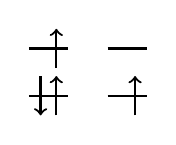
\begin{tikzpicture}[baseline={(current bounding box.center)}]
% lower MOs:
\draw[thick] (0,-0.6) -- (0.5,-0.6)%node[pos=0, left] {$a_2$}
;\draw[->, thick] (0.35, -0.85) -- (0.35, -0.35) ; 
 \draw[<-, thick] (0.15, -0.85) -- (0.15, -0.35) ;\draw[thick] (1,-0.6) -- (1.5,-0.6)%node[pos=1, right] {$b_2$}
;\draw[->, thick] (1.35, -0.85) -- (1.35, -0.35) ;
% upper MOs:
\draw[thick] (0,0) -- (0.5,0)%node[pos=0, left] {$b_2^{*}$}
;\draw[->, thick] (0.35, -0.25) -- (0.35, 0.25) ;\draw[thick] (1,0) -- (1.5,0)%node[pos=1, right] {$a_2^{*}$}
;;
\end{tikzpicture}
\quad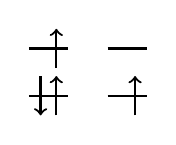
\begin{tikzpicture}[baseline={(current bounding box.center)}]
% lower MOs:
\draw[thick] (0,-0.6) -- (0.5,-0.6)%node[pos=0, left] {$a_2$}
;\draw[->, thick] (0.35, -0.85) -- (0.35, -0.35) ; 
 \draw[<-, thick] (0.15, -0.85) -- (0.15, -0.35) ;\draw[thick] (1,-0.6) -- (1.5,-0.6)%node[pos=1, right] {$b_2$}
;\draw[->, thick] (1.35, -0.85) -- (1.35, -0.35) ;
% upper MOs:
\draw[thick] (0,0) -- (0.5,0)%node[pos=0, left] {$b_2^{*}$}
;\draw[->, thick] (0.35, -0.25) -- (0.35, 0.25) ;\draw[thick] (1,0) -- (1.5,0)%node[pos=1, right] {$a_2^{*}$}
;;
\end{tikzpicture}\right) 
 + \left(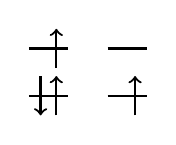
\begin{tikzpicture}[baseline={(current bounding box.center)}]
% lower MOs:
\draw[thick] (0,-0.6) -- (0.5,-0.6)%node[pos=0, left] {$a_2$}
;\draw[->, thick] (0.35, -0.85) -- (0.35, -0.35) ; 
 \draw[<-, thick] (0.15, -0.85) -- (0.15, -0.35) ;\draw[thick] (1,-0.6) -- (1.5,-0.6)%node[pos=1, right] {$b_2$}
;\draw[->, thick] (1.35, -0.85) -- (1.35, -0.35) ;
% upper MOs:
\draw[thick] (0,0) -- (0.5,0)%node[pos=0, left] {$b_2^{*}$}
;\draw[->, thick] (0.35, -0.25) -- (0.35, 0.25) ;\draw[thick] (1,0) -- (1.5,0)%node[pos=1, right] {$a_2^{*}$}
;;
\end{tikzpicture}
\quad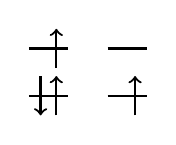
\begin{tikzpicture}[baseline={(current bounding box.center)}]
% lower MOs:
\draw[thick] (0,-0.6) -- (0.5,-0.6)%node[pos=0, left] {$a_2$}
;\draw[->, thick] (0.35, -0.85) -- (0.35, -0.35) ; 
 \draw[<-, thick] (0.15, -0.85) -- (0.15, -0.35) ;\draw[thick] (1,-0.6) -- (1.5,-0.6)%node[pos=1, right] {$b_2$}
;\draw[->, thick] (1.35, -0.85) -- (1.35, -0.35) ;
% upper MOs:
\draw[thick] (0,0) -- (0.5,0)%node[pos=0, left] {$b_2^{*}$}
;\draw[->, thick] (0.35, -0.25) -- (0.35, 0.25) ;\draw[thick] (1,0) -- (1.5,0)%node[pos=1, right] {$a_2^{*}$}
;;
\end{tikzpicture}\right) 
 + \left(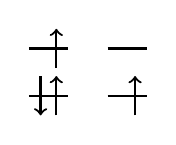
\begin{tikzpicture}[baseline={(current bounding box.center)}]
% lower MOs:
\draw[thick] (0,-0.6) -- (0.5,-0.6)%node[pos=0, left] {$a_2$}
;\draw[->, thick] (0.35, -0.85) -- (0.35, -0.35) ; 
 \draw[<-, thick] (0.15, -0.85) -- (0.15, -0.35) ;\draw[thick] (1,-0.6) -- (1.5,-0.6)%node[pos=1, right] {$b_2$}
;\draw[->, thick] (1.35, -0.85) -- (1.35, -0.35) ;
% upper MOs:
\draw[thick] (0,0) -- (0.5,0)%node[pos=0, left] {$b_2^{*}$}
;\draw[->, thick] (0.35, -0.25) -- (0.35, 0.25) ;\draw[thick] (1,0) -- (1.5,0)%node[pos=1, right] {$a_2^{*}$}
;;
\end{tikzpicture}
\quad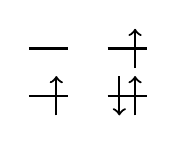
\begin{tikzpicture}[baseline={(current bounding box.center)}]
% lower MOs:
\draw[thick] (0,-0.6) -- (0.5,-0.6)%node[pos=0, left] {$a_2$}
;\draw[->, thick] (0.35, -0.85) -- (0.35, -0.35) ;\draw[thick] (1,-0.6) -- (1.5,-0.6)%node[pos=1, right] {$b_2$}
;\draw[->, thick] (1.35, -0.85) -- (1.35, -0.35) ; 
 \draw[<-, thick] (1.15, -0.85) -- (1.15, -0.35) ;
% upper MOs:
\draw[thick] (0,0) -- (0.5,0)%node[pos=0, left] {$b_2^{*}$}
;;\draw[thick] (1,0) -- (1.5,0)%node[pos=1, right] {$a_2^{*}$}
;\draw[->, thick] (1.35, -0.25) -- (1.35, 0.25) ;
\end{tikzpicture}\right) 
 + \left(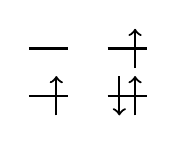
\begin{tikzpicture}[baseline={(current bounding box.center)}]
% lower MOs:
\draw[thick] (0,-0.6) -- (0.5,-0.6)%node[pos=0, left] {$a_2$}
;\draw[->, thick] (0.35, -0.85) -- (0.35, -0.35) ;\draw[thick] (1,-0.6) -- (1.5,-0.6)%node[pos=1, right] {$b_2$}
;\draw[->, thick] (1.35, -0.85) -- (1.35, -0.35) ; 
 \draw[<-, thick] (1.15, -0.85) -- (1.15, -0.35) ;
% upper MOs:
\draw[thick] (0,0) -- (0.5,0)%node[pos=0, left] {$b_2^{*}$}
;;\draw[thick] (1,0) -- (1.5,0)%node[pos=1, right] {$a_2^{*}$}
;\draw[->, thick] (1.35, -0.25) -- (1.35, 0.25) ;
\end{tikzpicture}
\quad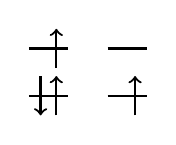
\begin{tikzpicture}[baseline={(current bounding box.center)}]
% lower MOs:
\draw[thick] (0,-0.6) -- (0.5,-0.6)%node[pos=0, left] {$a_2$}
;\draw[->, thick] (0.35, -0.85) -- (0.35, -0.35) ; 
 \draw[<-, thick] (0.15, -0.85) -- (0.15, -0.35) ;\draw[thick] (1,-0.6) -- (1.5,-0.6)%node[pos=1, right] {$b_2$}
;\draw[->, thick] (1.35, -0.85) -- (1.35, -0.35) ;
% upper MOs:
\draw[thick] (0,0) -- (0.5,0)%node[pos=0, left] {$b_2^{*}$}
;\draw[->, thick] (0.35, -0.25) -- (0.35, 0.25) ;\draw[thick] (1,0) -- (1.5,0)%node[pos=1, right] {$a_2^{*}$}
;;
\end{tikzpicture}\right) 
 \\[0.5cm] - \left(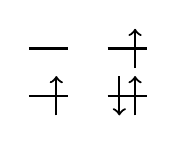
\begin{tikzpicture}[baseline={(current bounding box.center)}]
% lower MOs:
\draw[thick] (0,-0.6) -- (0.5,-0.6)%node[pos=0, left] {$a_2$}
;\draw[->, thick] (0.35, -0.85) -- (0.35, -0.35) ;\draw[thick] (1,-0.6) -- (1.5,-0.6)%node[pos=1, right] {$b_2$}
;\draw[->, thick] (1.35, -0.85) -- (1.35, -0.35) ; 
 \draw[<-, thick] (1.15, -0.85) -- (1.15, -0.35) ;
% upper MOs:
\draw[thick] (0,0) -- (0.5,0)%node[pos=0, left] {$b_2^{*}$}
;;\draw[thick] (1,0) -- (1.5,0)%node[pos=1, right] {$a_2^{*}$}
;\draw[->, thick] (1.35, -0.25) -- (1.35, 0.25) ;
\end{tikzpicture}
\quad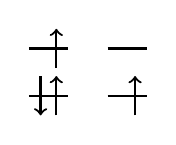
\begin{tikzpicture}[baseline={(current bounding box.center)}]
% lower MOs:
\draw[thick] (0,-0.6) -- (0.5,-0.6)%node[pos=0, left] {$a_2$}
;\draw[->, thick] (0.35, -0.85) -- (0.35, -0.35) ; 
 \draw[<-, thick] (0.15, -0.85) -- (0.15, -0.35) ;\draw[thick] (1,-0.6) -- (1.5,-0.6)%node[pos=1, right] {$b_2$}
;\draw[->, thick] (1.35, -0.85) -- (1.35, -0.35) ;
% upper MOs:
\draw[thick] (0,0) -- (0.5,0)%node[pos=0, left] {$b_2^{*}$}
;\draw[->, thick] (0.35, -0.25) -- (0.35, 0.25) ;\draw[thick] (1,0) -- (1.5,0)%node[pos=1, right] {$a_2^{*}$}
;;
\end{tikzpicture}\right) 
 - \left(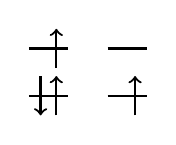
\begin{tikzpicture}[baseline={(current bounding box.center)}]
% lower MOs:
\draw[thick] (0,-0.6) -- (0.5,-0.6)%node[pos=0, left] {$a_2$}
;\draw[->, thick] (0.35, -0.85) -- (0.35, -0.35) ; 
 \draw[<-, thick] (0.15, -0.85) -- (0.15, -0.35) ;\draw[thick] (1,-0.6) -- (1.5,-0.6)%node[pos=1, right] {$b_2$}
;\draw[->, thick] (1.35, -0.85) -- (1.35, -0.35) ;
% upper MOs:
\draw[thick] (0,0) -- (0.5,0)%node[pos=0, left] {$b_2^{*}$}
;\draw[->, thick] (0.35, -0.25) -- (0.35, 0.25) ;\draw[thick] (1,0) -- (1.5,0)%node[pos=1, right] {$a_2^{*}$}
;;
\end{tikzpicture}
\quad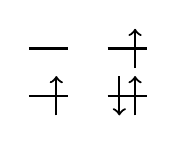
\begin{tikzpicture}[baseline={(current bounding box.center)}]
% lower MOs:
\draw[thick] (0,-0.6) -- (0.5,-0.6)%node[pos=0, left] {$a_2$}
;\draw[->, thick] (0.35, -0.85) -- (0.35, -0.35) ;\draw[thick] (1,-0.6) -- (1.5,-0.6)%node[pos=1, right] {$b_2$}
;\draw[->, thick] (1.35, -0.85) -- (1.35, -0.35) ; 
 \draw[<-, thick] (1.15, -0.85) -- (1.15, -0.35) ;
% upper MOs:
\draw[thick] (0,0) -- (0.5,0)%node[pos=0, left] {$b_2^{*}$}
;;\draw[thick] (1,0) -- (1.5,0)%node[pos=1, right] {$a_2^{*}$}
;\draw[->, thick] (1.35, -0.25) -- (1.35, 0.25) ;
\end{tikzpicture}\right) 
 - \left(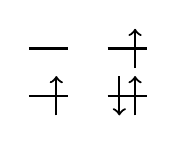
\begin{tikzpicture}[baseline={(current bounding box.center)}]
% lower MOs:
\draw[thick] (0,-0.6) -- (0.5,-0.6)%node[pos=0, left] {$a_2$}
;\draw[->, thick] (0.35, -0.85) -- (0.35, -0.35) ;\draw[thick] (1,-0.6) -- (1.5,-0.6)%node[pos=1, right] {$b_2$}
;\draw[->, thick] (1.35, -0.85) -- (1.35, -0.35) ; 
 \draw[<-, thick] (1.15, -0.85) -- (1.15, -0.35) ;
% upper MOs:
\draw[thick] (0,0) -- (0.5,0)%node[pos=0, left] {$b_2^{*}$}
;;\draw[thick] (1,0) -- (1.5,0)%node[pos=1, right] {$a_2^{*}$}
;\draw[->, thick] (1.35, -0.25) -- (1.35, 0.25) ;
\end{tikzpicture}
\quad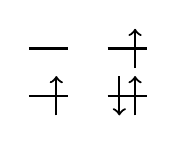
\begin{tikzpicture}[baseline={(current bounding box.center)}]
% lower MOs:
\draw[thick] (0,-0.6) -- (0.5,-0.6)%node[pos=0, left] {$a_2$}
;\draw[->, thick] (0.35, -0.85) -- (0.35, -0.35) ;\draw[thick] (1,-0.6) -- (1.5,-0.6)%node[pos=1, right] {$b_2$}
;\draw[->, thick] (1.35, -0.85) -- (1.35, -0.35) ; 
 \draw[<-, thick] (1.15, -0.85) -- (1.15, -0.35) ;
% upper MOs:
\draw[thick] (0,0) -- (0.5,0)%node[pos=0, left] {$b_2^{*}$}
;;\draw[thick] (1,0) -- (1.5,0)%node[pos=1, right] {$a_2^{*}$}
;\draw[->, thick] (1.35, -0.25) -- (1.35, 0.25) ;
\end{tikzpicture}\right) 
 - \left(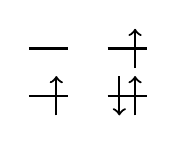
\begin{tikzpicture}[baseline={(current bounding box.center)}]
% lower MOs:
\draw[thick] (0,-0.6) -- (0.5,-0.6)%node[pos=0, left] {$a_2$}
;\draw[->, thick] (0.35, -0.85) -- (0.35, -0.35) ;\draw[thick] (1,-0.6) -- (1.5,-0.6)%node[pos=1, right] {$b_2$}
;\draw[->, thick] (1.35, -0.85) -- (1.35, -0.35) ; 
 \draw[<-, thick] (1.15, -0.85) -- (1.15, -0.35) ;
% upper MOs:
\draw[thick] (0,0) -- (0.5,0)%node[pos=0, left] {$b_2^{*}$}
;;\draw[thick] (1,0) -- (1.5,0)%node[pos=1, right] {$a_2^{*}$}
;\draw[->, thick] (1.35, -0.25) -- (1.35, 0.25) ;
\end{tikzpicture}
\quad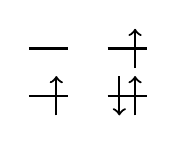
\begin{tikzpicture}[baseline={(current bounding box.center)}]
% lower MOs:
\draw[thick] (0,-0.6) -- (0.5,-0.6)%node[pos=0, left] {$a_2$}
;\draw[->, thick] (0.35, -0.85) -- (0.35, -0.35) ;\draw[thick] (1,-0.6) -- (1.5,-0.6)%node[pos=1, right] {$b_2$}
;\draw[->, thick] (1.35, -0.85) -- (1.35, -0.35) ; 
 \draw[<-, thick] (1.15, -0.85) -- (1.15, -0.35) ;
% upper MOs:
\draw[thick] (0,0) -- (0.5,0)%node[pos=0, left] {$b_2^{*}$}
;;\draw[thick] (1,0) -- (1.5,0)%node[pos=1, right] {$a_2^{*}$}
;\draw[->, thick] (1.35, -0.25) -- (1.35, 0.25) ;
\end{tikzpicture}\right) 
\end{array}\]
monomer ci vectors:
$$\begin{array}{c}
+\left|\underbrace{(b_2^{\mathsf{l}})^{1}(b_2^{*l})^{1}(a_2^{\mathsf{l}})^{2}(a_2^{*l})^{0}}_{a_1^{\mathsf{l}}}\right| \otimes{} \left|\underbrace{(b_2^{\mathsf{r}})^{1}(b_2^{*r})^{1}(a_2^{\mathsf{r}})^{2}(a_2^{*r})^{0}}_{a_1^{\mathsf{r}}}\right| +\left|\underbrace{(b_2^{\mathsf{l}})^{1}(b_2^{*l})^{1}(a_2^{\mathsf{l}})^{2}(a_2^{*l})^{0}}_{a_1^{\mathsf{l}}}\right| \otimes{} \left|\underbrace{(b_2^{\mathsf{r}})^{1}(b_2^{*r})^{1}(a_2^{\mathsf{r}})^{2}(a_2^{*r})^{0}}_{a_1^{\mathsf{r}}}\right| \\[0.5cm] +\left|\underbrace{(b_2^{\mathsf{l}})^{1}(b_2^{*l})^{1}(a_2^{\mathsf{l}})^{2}(a_2^{*l})^{0}}_{a_1^{\mathsf{l}}}\right| \otimes{} \left|\underbrace{(b_2^{\mathsf{r}})^{2}(b_2^{*r})^{0}(a_2^{\mathsf{r}})^{1}(a_2^{*r})^{1}}_{a_1^{\mathsf{r}}}\right| +\left|\underbrace{(b_2^{\mathsf{l}})^{2}(b_2^{*l})^{0}(a_2^{\mathsf{l}})^{1}(a_2^{*l})^{1}}_{a_1^{\mathsf{l}}}\right| \otimes{} \left|\underbrace{(b_2^{\mathsf{r}})^{1}(b_2^{*r})^{1}(a_2^{\mathsf{r}})^{2}(a_2^{*r})^{0}}_{a_1^{\mathsf{r}}}\right| \\[0.5cm] -\left|\underbrace{(b_2^{\mathsf{l}})^{2}(b_2^{*l})^{0}(a_2^{\mathsf{l}})^{1}(a_2^{*l})^{1}}_{a_1^{\mathsf{l}}}\right| \otimes{} \left|\underbrace{(b_2^{\mathsf{r}})^{1}(b_2^{*r})^{1}(a_2^{\mathsf{r}})^{2}(a_2^{*r})^{0}}_{a_1^{\mathsf{r}}}\right| -\left|\underbrace{(b_2^{\mathsf{l}})^{1}(b_2^{*l})^{1}(a_2^{\mathsf{l}})^{2}(a_2^{*l})^{0}}_{a_1^{\mathsf{l}}}\right| \otimes{} \left|\underbrace{(b_2^{\mathsf{r}})^{2}(b_2^{*r})^{0}(a_2^{\mathsf{r}})^{1}(a_2^{*r})^{1}}_{a_1^{\mathsf{r}}}\right| \\[0.5cm] -\left|\underbrace{(b_2^{\mathsf{l}})^{2}(b_2^{*l})^{0}(a_2^{\mathsf{l}})^{1}(a_2^{*l})^{1}}_{a_1^{\mathsf{l}}}\right| \otimes{} \left|\underbrace{(b_2^{\mathsf{r}})^{2}(b_2^{*r})^{0}(a_2^{\mathsf{r}})^{1}(a_2^{*r})^{1}}_{a_1^{\mathsf{r}}}\right| -\left|\underbrace{(b_2^{\mathsf{l}})^{2}(b_2^{*l})^{0}(a_2^{\mathsf{l}})^{1}(a_2^{*l})^{1}}_{a_1^{\mathsf{l}}}\right| \otimes{} \left|\underbrace{(b_2^{\mathsf{r}})^{2}(b_2^{*r})^{0}(a_2^{\mathsf{r}})^{1}(a_2^{*r})^{1}}_{a_1^{\mathsf{r}}}\right|
\end{array}$$substitution by dimer orbitals:
$$+\left|\underbrace{(+a_{g}+b_u)^{1}(+a_g^{*}+b_u^{*})^{1}(+a_{u}+b_g)^{2}(+a_u^{*}+b_g^{*})^{0}}_{a_1^{\mathsf{l}}}\right| \otimes{} \left|\underbrace{(-a_{g}+b_u)^{1}(-a_g^{*}+b_u^{*})^{1}(+a_{u}-b_g)^{2}(+a_u^{*}-b_g^{*})^{0}}_{a_1^{\mathsf{r}}}\right| + \hdots $$(multiplied out and summed up) dimer ci vectors:

\begin{multline*}\begin{array}{c}
+2 \cdot \left|\underbrace{(a_{g})^{1}(b_u)^{1}(a_{u})^{2}(b_g)^{2}(a_g^{*})^{1}(b_u^{*})^{1}(a_u^{*})^{0}(b_g^{*})^{0}}_{a_{g}}\right| -2 \cdot \left|\underbrace{(a_{g})^{2}(b_u)^{2}(a_{u})^{1}(b_g)^{1}(a_g^{*})^{0}(b_u^{*})^{0}(a_u^{*})^{1}(b_g^{*})^{1}}_{a_{g}}\right|
\end{array}\end{multline*}


\vspace{0.5cm}

\newpage

\subsection{\boldmath $i^3 a_1 \otimes e^3 a_1 - e^3 a_1 \otimes i^3 a_1$}
\[i^3 a_1 \otimes e^3 a_1 - e^3 a_1 \otimes i^3 a_1\]
\[\begin{array}{c}
+ \left(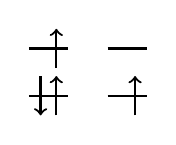
\begin{tikzpicture}[baseline={(current bounding box.center)}]
% lower MOs:
\draw[thick] (0,-0.6) -- (0.5,-0.6)%node[pos=0, left] {$a_2$}
;\draw[->, thick] (0.35, -0.85) -- (0.35, -0.35) ; 
 \draw[<-, thick] (0.15, -0.85) -- (0.15, -0.35) ;\draw[thick] (1,-0.6) -- (1.5,-0.6)%node[pos=1, right] {$b_2$}
;\draw[->, thick] (1.35, -0.85) -- (1.35, -0.35) ;
% upper MOs:
\draw[thick] (0,0) -- (0.5,0)%node[pos=0, left] {$b_2^{*}$}
;\draw[->, thick] (0.35, -0.25) -- (0.35, 0.25) ;\draw[thick] (1,0) -- (1.5,0)%node[pos=1, right] {$a_2^{*}$}
;;
\end{tikzpicture}
\quad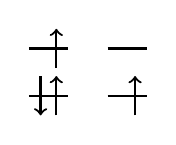
\begin{tikzpicture}[baseline={(current bounding box.center)}]
% lower MOs:
\draw[thick] (0,-0.6) -- (0.5,-0.6)%node[pos=0, left] {$a_2$}
;\draw[->, thick] (0.35, -0.85) -- (0.35, -0.35) ; 
 \draw[<-, thick] (0.15, -0.85) -- (0.15, -0.35) ;\draw[thick] (1,-0.6) -- (1.5,-0.6)%node[pos=1, right] {$b_2$}
;\draw[->, thick] (1.35, -0.85) -- (1.35, -0.35) ;
% upper MOs:
\draw[thick] (0,0) -- (0.5,0)%node[pos=0, left] {$b_2^{*}$}
;\draw[->, thick] (0.35, -0.25) -- (0.35, 0.25) ;\draw[thick] (1,0) -- (1.5,0)%node[pos=1, right] {$a_2^{*}$}
;;
\end{tikzpicture}\right) 
 - \left(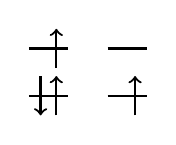
\begin{tikzpicture}[baseline={(current bounding box.center)}]
% lower MOs:
\draw[thick] (0,-0.6) -- (0.5,-0.6)%node[pos=0, left] {$a_2$}
;\draw[->, thick] (0.35, -0.85) -- (0.35, -0.35) ; 
 \draw[<-, thick] (0.15, -0.85) -- (0.15, -0.35) ;\draw[thick] (1,-0.6) -- (1.5,-0.6)%node[pos=1, right] {$b_2$}
;\draw[->, thick] (1.35, -0.85) -- (1.35, -0.35) ;
% upper MOs:
\draw[thick] (0,0) -- (0.5,0)%node[pos=0, left] {$b_2^{*}$}
;\draw[->, thick] (0.35, -0.25) -- (0.35, 0.25) ;\draw[thick] (1,0) -- (1.5,0)%node[pos=1, right] {$a_2^{*}$}
;;
\end{tikzpicture}
\quad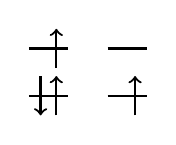
\begin{tikzpicture}[baseline={(current bounding box.center)}]
% lower MOs:
\draw[thick] (0,-0.6) -- (0.5,-0.6)%node[pos=0, left] {$a_2$}
;\draw[->, thick] (0.35, -0.85) -- (0.35, -0.35) ; 
 \draw[<-, thick] (0.15, -0.85) -- (0.15, -0.35) ;\draw[thick] (1,-0.6) -- (1.5,-0.6)%node[pos=1, right] {$b_2$}
;\draw[->, thick] (1.35, -0.85) -- (1.35, -0.35) ;
% upper MOs:
\draw[thick] (0,0) -- (0.5,0)%node[pos=0, left] {$b_2^{*}$}
;\draw[->, thick] (0.35, -0.25) -- (0.35, 0.25) ;\draw[thick] (1,0) -- (1.5,0)%node[pos=1, right] {$a_2^{*}$}
;;
\end{tikzpicture}\right) 
 + \left(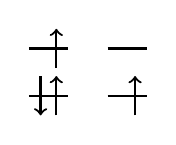
\begin{tikzpicture}[baseline={(current bounding box.center)}]
% lower MOs:
\draw[thick] (0,-0.6) -- (0.5,-0.6)%node[pos=0, left] {$a_2$}
;\draw[->, thick] (0.35, -0.85) -- (0.35, -0.35) ; 
 \draw[<-, thick] (0.15, -0.85) -- (0.15, -0.35) ;\draw[thick] (1,-0.6) -- (1.5,-0.6)%node[pos=1, right] {$b_2$}
;\draw[->, thick] (1.35, -0.85) -- (1.35, -0.35) ;
% upper MOs:
\draw[thick] (0,0) -- (0.5,0)%node[pos=0, left] {$b_2^{*}$}
;\draw[->, thick] (0.35, -0.25) -- (0.35, 0.25) ;\draw[thick] (1,0) -- (1.5,0)%node[pos=1, right] {$a_2^{*}$}
;;
\end{tikzpicture}
\quad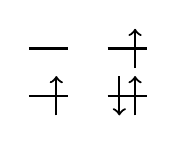
\begin{tikzpicture}[baseline={(current bounding box.center)}]
% lower MOs:
\draw[thick] (0,-0.6) -- (0.5,-0.6)%node[pos=0, left] {$a_2$}
;\draw[->, thick] (0.35, -0.85) -- (0.35, -0.35) ;\draw[thick] (1,-0.6) -- (1.5,-0.6)%node[pos=1, right] {$b_2$}
;\draw[->, thick] (1.35, -0.85) -- (1.35, -0.35) ; 
 \draw[<-, thick] (1.15, -0.85) -- (1.15, -0.35) ;
% upper MOs:
\draw[thick] (0,0) -- (0.5,0)%node[pos=0, left] {$b_2^{*}$}
;;\draw[thick] (1,0) -- (1.5,0)%node[pos=1, right] {$a_2^{*}$}
;\draw[->, thick] (1.35, -0.25) -- (1.35, 0.25) ;
\end{tikzpicture}\right) 
 - \left(\begin{tikzpicture}[baseline={(current bounding box.center)}]
% lower MOs:
\draw[thick] (0,-0.6) -- (0.5,-0.6)%node[pos=0, left] {$a_2$}
;\draw[->, thick] (0.35, -0.85) -- (0.35, -0.35) ;\draw[thick] (1,-0.6) -- (1.5,-0.6)%node[pos=1, right] {$b_2$}
;\draw[->, thick] (1.35, -0.85) -- (1.35, -0.35) ; 
 \draw[<-, thick] (1.15, -0.85) -- (1.15, -0.35) ;
% upper MOs:
\draw[thick] (0,0) -- (0.5,0)%node[pos=0, left] {$b_2^{*}$}
;;\draw[thick] (1,0) -- (1.5,0)%node[pos=1, right] {$a_2^{*}$}
;\draw[->, thick] (1.35, -0.25) -- (1.35, 0.25) ;
\end{tikzpicture}
\quad\begin{tikzpicture}[baseline={(current bounding box.center)}]
% lower MOs:
\draw[thick] (0,-0.6) -- (0.5,-0.6)%node[pos=0, left] {$a_2$}
;\draw[->, thick] (0.35, -0.85) -- (0.35, -0.35) ; 
 \draw[<-, thick] (0.15, -0.85) -- (0.15, -0.35) ;\draw[thick] (1,-0.6) -- (1.5,-0.6)%node[pos=1, right] {$b_2$}
;\draw[->, thick] (1.35, -0.85) -- (1.35, -0.35) ;
% upper MOs:
\draw[thick] (0,0) -- (0.5,0)%node[pos=0, left] {$b_2^{*}$}
;\draw[->, thick] (0.35, -0.25) -- (0.35, 0.25) ;\draw[thick] (1,0) -- (1.5,0)%node[pos=1, right] {$a_2^{*}$}
;;
\end{tikzpicture}\right) 
 \\[0.5cm] - \left(\begin{tikzpicture}[baseline={(current bounding box.center)}]
% lower MOs:
\draw[thick] (0,-0.6) -- (0.5,-0.6)%node[pos=0, left] {$a_2$}
;\draw[->, thick] (0.35, -0.85) -- (0.35, -0.35) ;\draw[thick] (1,-0.6) -- (1.5,-0.6)%node[pos=1, right] {$b_2$}
;\draw[->, thick] (1.35, -0.85) -- (1.35, -0.35) ; 
 \draw[<-, thick] (1.15, -0.85) -- (1.15, -0.35) ;
% upper MOs:
\draw[thick] (0,0) -- (0.5,0)%node[pos=0, left] {$b_2^{*}$}
;;\draw[thick] (1,0) -- (1.5,0)%node[pos=1, right] {$a_2^{*}$}
;\draw[->, thick] (1.35, -0.25) -- (1.35, 0.25) ;
\end{tikzpicture}
\quad\begin{tikzpicture}[baseline={(current bounding box.center)}]
% lower MOs:
\draw[thick] (0,-0.6) -- (0.5,-0.6)%node[pos=0, left] {$a_2$}
;\draw[->, thick] (0.35, -0.85) -- (0.35, -0.35) ; 
 \draw[<-, thick] (0.15, -0.85) -- (0.15, -0.35) ;\draw[thick] (1,-0.6) -- (1.5,-0.6)%node[pos=1, right] {$b_2$}
;\draw[->, thick] (1.35, -0.85) -- (1.35, -0.35) ;
% upper MOs:
\draw[thick] (0,0) -- (0.5,0)%node[pos=0, left] {$b_2^{*}$}
;\draw[->, thick] (0.35, -0.25) -- (0.35, 0.25) ;\draw[thick] (1,0) -- (1.5,0)%node[pos=1, right] {$a_2^{*}$}
;;
\end{tikzpicture}\right) 
 + \left(\begin{tikzpicture}[baseline={(current bounding box.center)}]
% lower MOs:
\draw[thick] (0,-0.6) -- (0.5,-0.6)%node[pos=0, left] {$a_2$}
;\draw[->, thick] (0.35, -0.85) -- (0.35, -0.35) ; 
 \draw[<-, thick] (0.15, -0.85) -- (0.15, -0.35) ;\draw[thick] (1,-0.6) -- (1.5,-0.6)%node[pos=1, right] {$b_2$}
;\draw[->, thick] (1.35, -0.85) -- (1.35, -0.35) ;
% upper MOs:
\draw[thick] (0,0) -- (0.5,0)%node[pos=0, left] {$b_2^{*}$}
;\draw[->, thick] (0.35, -0.25) -- (0.35, 0.25) ;\draw[thick] (1,0) -- (1.5,0)%node[pos=1, right] {$a_2^{*}$}
;;
\end{tikzpicture}
\quad\begin{tikzpicture}[baseline={(current bounding box.center)}]
% lower MOs:
\draw[thick] (0,-0.6) -- (0.5,-0.6)%node[pos=0, left] {$a_2$}
;\draw[->, thick] (0.35, -0.85) -- (0.35, -0.35) ;\draw[thick] (1,-0.6) -- (1.5,-0.6)%node[pos=1, right] {$b_2$}
;\draw[->, thick] (1.35, -0.85) -- (1.35, -0.35) ; 
 \draw[<-, thick] (1.15, -0.85) -- (1.15, -0.35) ;
% upper MOs:
\draw[thick] (0,0) -- (0.5,0)%node[pos=0, left] {$b_2^{*}$}
;;\draw[thick] (1,0) -- (1.5,0)%node[pos=1, right] {$a_2^{*}$}
;\draw[->, thick] (1.35, -0.25) -- (1.35, 0.25) ;
\end{tikzpicture}\right) 
 - \left(\begin{tikzpicture}[baseline={(current bounding box.center)}]
% lower MOs:
\draw[thick] (0,-0.6) -- (0.5,-0.6)%node[pos=0, left] {$a_2$}
;\draw[->, thick] (0.35, -0.85) -- (0.35, -0.35) ;\draw[thick] (1,-0.6) -- (1.5,-0.6)%node[pos=1, right] {$b_2$}
;\draw[->, thick] (1.35, -0.85) -- (1.35, -0.35) ; 
 \draw[<-, thick] (1.15, -0.85) -- (1.15, -0.35) ;
% upper MOs:
\draw[thick] (0,0) -- (0.5,0)%node[pos=0, left] {$b_2^{*}$}
;;\draw[thick] (1,0) -- (1.5,0)%node[pos=1, right] {$a_2^{*}$}
;\draw[->, thick] (1.35, -0.25) -- (1.35, 0.25) ;
\end{tikzpicture}
\quad\begin{tikzpicture}[baseline={(current bounding box.center)}]
% lower MOs:
\draw[thick] (0,-0.6) -- (0.5,-0.6)%node[pos=0, left] {$a_2$}
;\draw[->, thick] (0.35, -0.85) -- (0.35, -0.35) ;\draw[thick] (1,-0.6) -- (1.5,-0.6)%node[pos=1, right] {$b_2$}
;\draw[->, thick] (1.35, -0.85) -- (1.35, -0.35) ; 
 \draw[<-, thick] (1.15, -0.85) -- (1.15, -0.35) ;
% upper MOs:
\draw[thick] (0,0) -- (0.5,0)%node[pos=0, left] {$b_2^{*}$}
;;\draw[thick] (1,0) -- (1.5,0)%node[pos=1, right] {$a_2^{*}$}
;\draw[->, thick] (1.35, -0.25) -- (1.35, 0.25) ;
\end{tikzpicture}\right) 
 + \left(\begin{tikzpicture}[baseline={(current bounding box.center)}]
% lower MOs:
\draw[thick] (0,-0.6) -- (0.5,-0.6)%node[pos=0, left] {$a_2$}
;\draw[->, thick] (0.35, -0.85) -- (0.35, -0.35) ;\draw[thick] (1,-0.6) -- (1.5,-0.6)%node[pos=1, right] {$b_2$}
;\draw[->, thick] (1.35, -0.85) -- (1.35, -0.35) ; 
 \draw[<-, thick] (1.15, -0.85) -- (1.15, -0.35) ;
% upper MOs:
\draw[thick] (0,0) -- (0.5,0)%node[pos=0, left] {$b_2^{*}$}
;;\draw[thick] (1,0) -- (1.5,0)%node[pos=1, right] {$a_2^{*}$}
;\draw[->, thick] (1.35, -0.25) -- (1.35, 0.25) ;
\end{tikzpicture}
\quad\begin{tikzpicture}[baseline={(current bounding box.center)}]
% lower MOs:
\draw[thick] (0,-0.6) -- (0.5,-0.6)%node[pos=0, left] {$a_2$}
;\draw[->, thick] (0.35, -0.85) -- (0.35, -0.35) ;\draw[thick] (1,-0.6) -- (1.5,-0.6)%node[pos=1, right] {$b_2$}
;\draw[->, thick] (1.35, -0.85) -- (1.35, -0.35) ; 
 \draw[<-, thick] (1.15, -0.85) -- (1.15, -0.35) ;
% upper MOs:
\draw[thick] (0,0) -- (0.5,0)%node[pos=0, left] {$b_2^{*}$}
;;\draw[thick] (1,0) -- (1.5,0)%node[pos=1, right] {$a_2^{*}$}
;\draw[->, thick] (1.35, -0.25) -- (1.35, 0.25) ;
\end{tikzpicture}\right) 
\end{array}\]
monomer ci vectors:
$$\begin{array}{c}
+\left|\underbrace{(b_2^{\mathsf{l}})^{1}(b_2^{*l})^{1}(a_2^{\mathsf{l}})^{2}(a_2^{*l})^{0}}_{a_1^{\mathsf{l}}}\right| \otimes{} \left|\underbrace{(b_2^{\mathsf{r}})^{1}(b_2^{*r})^{1}(a_2^{\mathsf{r}})^{2}(a_2^{*r})^{0}}_{a_1^{\mathsf{r}}}\right| -\left|\underbrace{(b_2^{\mathsf{l}})^{1}(b_2^{*l})^{1}(a_2^{\mathsf{l}})^{2}(a_2^{*l})^{0}}_{a_1^{\mathsf{l}}}\right| \otimes{} \left|\underbrace{(b_2^{\mathsf{r}})^{1}(b_2^{*r})^{1}(a_2^{\mathsf{r}})^{2}(a_2^{*r})^{0}}_{a_1^{\mathsf{r}}}\right| \\[0.5cm] +\left|\underbrace{(b_2^{\mathsf{l}})^{1}(b_2^{*l})^{1}(a_2^{\mathsf{l}})^{2}(a_2^{*l})^{0}}_{a_1^{\mathsf{l}}}\right| \otimes{} \left|\underbrace{(b_2^{\mathsf{r}})^{2}(b_2^{*r})^{0}(a_2^{\mathsf{r}})^{1}(a_2^{*r})^{1}}_{a_1^{\mathsf{r}}}\right| -\left|\underbrace{(b_2^{\mathsf{l}})^{2}(b_2^{*l})^{0}(a_2^{\mathsf{l}})^{1}(a_2^{*l})^{1}}_{a_1^{\mathsf{l}}}\right| \otimes{} \left|\underbrace{(b_2^{\mathsf{r}})^{1}(b_2^{*r})^{1}(a_2^{\mathsf{r}})^{2}(a_2^{*r})^{0}}_{a_1^{\mathsf{r}}}\right| \\[0.5cm] -\left|\underbrace{(b_2^{\mathsf{l}})^{2}(b_2^{*l})^{0}(a_2^{\mathsf{l}})^{1}(a_2^{*l})^{1}}_{a_1^{\mathsf{l}}}\right| \otimes{} \left|\underbrace{(b_2^{\mathsf{r}})^{1}(b_2^{*r})^{1}(a_2^{\mathsf{r}})^{2}(a_2^{*r})^{0}}_{a_1^{\mathsf{r}}}\right| +\left|\underbrace{(b_2^{\mathsf{l}})^{1}(b_2^{*l})^{1}(a_2^{\mathsf{l}})^{2}(a_2^{*l})^{0}}_{a_1^{\mathsf{l}}}\right| \otimes{} \left|\underbrace{(b_2^{\mathsf{r}})^{2}(b_2^{*r})^{0}(a_2^{\mathsf{r}})^{1}(a_2^{*r})^{1}}_{a_1^{\mathsf{r}}}\right| \\[0.5cm] -\left|\underbrace{(b_2^{\mathsf{l}})^{2}(b_2^{*l})^{0}(a_2^{\mathsf{l}})^{1}(a_2^{*l})^{1}}_{a_1^{\mathsf{l}}}\right| \otimes{} \left|\underbrace{(b_2^{\mathsf{r}})^{2}(b_2^{*r})^{0}(a_2^{\mathsf{r}})^{1}(a_2^{*r})^{1}}_{a_1^{\mathsf{r}}}\right| +\left|\underbrace{(b_2^{\mathsf{l}})^{2}(b_2^{*l})^{0}(a_2^{\mathsf{l}})^{1}(a_2^{*l})^{1}}_{a_1^{\mathsf{l}}}\right| \otimes{} \left|\underbrace{(b_2^{\mathsf{r}})^{2}(b_2^{*r})^{0}(a_2^{\mathsf{r}})^{1}(a_2^{*r})^{1}}_{a_1^{\mathsf{r}}}\right|
\end{array}$$substitution by dimer orbitals:
$$+\left|\underbrace{(+a_{g}+b_u)^{1}(+a_g^{*}+b_u^{*})^{1}(+a_{u}+b_g)^{2}(+a_u^{*}+b_g^{*})^{0}}_{a_1^{\mathsf{l}}}\right| \otimes{} \left|\underbrace{(-a_{g}+b_u)^{1}(-a_g^{*}+b_u^{*})^{1}(+a_{u}-b_g)^{2}(+a_u^{*}-b_g^{*})^{0}}_{a_1^{\mathsf{r}}}\right| + \hdots $$(multiplied out and summed up) dimer ci vectors:

\begin{multline*}\begin{array}{c}
+4 \cdot \left|\underbrace{(a_{g})^{1}(b_u)^{2}(a_{u})^{2}(b_g)^{1}(a_g^{*})^{1}(b_u^{*})^{0}(a_u^{*})^{1}(b_g^{*})^{0}}_{b_u}\right| +4 \cdot \left|\underbrace{(a_{g})^{1}(b_u)^{2}(a_{u})^{1}(b_g)^{2}(a_g^{*})^{1}(b_u^{*})^{0}(a_u^{*})^{0}(b_g^{*})^{1}}_{b_u}\right| \\[0.5cm] -4 \cdot \left|\underbrace{(a_{g})^{1}(b_u)^{2}(a_{u})^{2}(b_g)^{1}(a_g^{*})^{0}(b_u^{*})^{1}(a_u^{*})^{0}(b_g^{*})^{1}}_{b_u}\right| -4 \cdot \left|\underbrace{(a_{g})^{1}(b_u)^{2}(a_{u})^{1}(b_g)^{2}(a_g^{*})^{0}(b_u^{*})^{1}(a_u^{*})^{1}(b_g^{*})^{0}}_{b_u}\right| \\[0.5cm] -4 \cdot \left|\underbrace{(a_{g})^{2}(b_u)^{1}(a_{u})^{2}(b_g)^{1}(a_g^{*})^{1}(b_u^{*})^{0}(a_u^{*})^{0}(b_g^{*})^{1}}_{b_u}\right| -4 \cdot \left|\underbrace{(a_{g})^{2}(b_u)^{1}(a_{u})^{1}(b_g)^{2}(a_g^{*})^{1}(b_u^{*})^{0}(a_u^{*})^{1}(b_g^{*})^{0}}_{b_u}\right| \\[0.5cm] +4 \cdot \left|\underbrace{(a_{g})^{2}(b_u)^{1}(a_{u})^{2}(b_g)^{1}(a_g^{*})^{0}(b_u^{*})^{1}(a_u^{*})^{1}(b_g^{*})^{0}}_{b_u}\right| +4 \cdot \left|\underbrace{(a_{g})^{2}(b_u)^{1}(a_{u})^{1}(b_g)^{2}(a_g^{*})^{0}(b_u^{*})^{1}(a_u^{*})^{0}(b_g^{*})^{1}}_{b_u}\right|
\end{array}\end{multline*}


\vspace{0.5cm}

\newpage

\subsection{\boldmath $i^3 a_1 \otimes i^3 b_{1} + i^3 b_{1} \otimes i^3 a_1$}
\[i^3 a_1 \otimes i^3 b_{1} + i^3 b_{1} \otimes i^3 a_1\]
\[\begin{array}{c}
+ \left(\begin{tikzpicture}[baseline={(current bounding box.center)}]
% lower MOs:
\draw[thick] (0,-0.6) -- (0.5,-0.6)%node[pos=0, left] {$a_2$}
;\draw[->, thick] (0.35, -0.85) -- (0.35, -0.35) ; 
 \draw[<-, thick] (0.15, -0.85) -- (0.15, -0.35) ;\draw[thick] (1,-0.6) -- (1.5,-0.6)%node[pos=1, right] {$b_2$}
;\draw[->, thick] (1.35, -0.85) -- (1.35, -0.35) ;
% upper MOs:
\draw[thick] (0,0) -- (0.5,0)%node[pos=0, left] {$b_2^{*}$}
;\draw[->, thick] (0.35, -0.25) -- (0.35, 0.25) ;\draw[thick] (1,0) -- (1.5,0)%node[pos=1, right] {$a_2^{*}$}
;;
\end{tikzpicture}
\quad\begin{tikzpicture}[baseline={(current bounding box.center)}]
% lower MOs:
\draw[thick] (0,-0.6) -- (0.5,-0.6)%node[pos=0, left] {$a_2$}
;\draw[->, thick] (0.35, -0.85) -- (0.35, -0.35) ;\draw[thick] (1,-0.6) -- (1.5,-0.6)%node[pos=1, right] {$b_2$}
;\draw[->, thick] (1.35, -0.85) -- (1.35, -0.35) ; 
 \draw[<-, thick] (1.15, -0.85) -- (1.15, -0.35) ;
% upper MOs:
\draw[thick] (0,0) -- (0.5,0)%node[pos=0, left] {$b_2^{*}$}
;\draw[->, thick] (0.35, -0.25) -- (0.35, 0.25) ;\draw[thick] (1,0) -- (1.5,0)%node[pos=1, right] {$a_2^{*}$}
;;
\end{tikzpicture}\right) 
 + \left(\begin{tikzpicture}[baseline={(current bounding box.center)}]
% lower MOs:
\draw[thick] (0,-0.6) -- (0.5,-0.6)%node[pos=0, left] {$a_2$}
;\draw[->, thick] (0.35, -0.85) -- (0.35, -0.35) ;\draw[thick] (1,-0.6) -- (1.5,-0.6)%node[pos=1, right] {$b_2$}
;\draw[->, thick] (1.35, -0.85) -- (1.35, -0.35) ; 
 \draw[<-, thick] (1.15, -0.85) -- (1.15, -0.35) ;
% upper MOs:
\draw[thick] (0,0) -- (0.5,0)%node[pos=0, left] {$b_2^{*}$}
;\draw[->, thick] (0.35, -0.25) -- (0.35, 0.25) ;\draw[thick] (1,0) -- (1.5,0)%node[pos=1, right] {$a_2^{*}$}
;;
\end{tikzpicture}
\quad\begin{tikzpicture}[baseline={(current bounding box.center)}]
% lower MOs:
\draw[thick] (0,-0.6) -- (0.5,-0.6)%node[pos=0, left] {$a_2$}
;\draw[->, thick] (0.35, -0.85) -- (0.35, -0.35) ; 
 \draw[<-, thick] (0.15, -0.85) -- (0.15, -0.35) ;\draw[thick] (1,-0.6) -- (1.5,-0.6)%node[pos=1, right] {$b_2$}
;\draw[->, thick] (1.35, -0.85) -- (1.35, -0.35) ;
% upper MOs:
\draw[thick] (0,0) -- (0.5,0)%node[pos=0, left] {$b_2^{*}$}
;\draw[->, thick] (0.35, -0.25) -- (0.35, 0.25) ;\draw[thick] (1,0) -- (1.5,0)%node[pos=1, right] {$a_2^{*}$}
;;
\end{tikzpicture}\right) 
 - \left(\begin{tikzpicture}[baseline={(current bounding box.center)}]
% lower MOs:
\draw[thick] (0,-0.6) -- (0.5,-0.6)%node[pos=0, left] {$a_2$}
;\draw[->, thick] (0.35, -0.85) -- (0.35, -0.35) ; 
 \draw[<-, thick] (0.15, -0.85) -- (0.15, -0.35) ;\draw[thick] (1,-0.6) -- (1.5,-0.6)%node[pos=1, right] {$b_2$}
;\draw[->, thick] (1.35, -0.85) -- (1.35, -0.35) ;
% upper MOs:
\draw[thick] (0,0) -- (0.5,0)%node[pos=0, left] {$b_2^{*}$}
;\draw[->, thick] (0.35, -0.25) -- (0.35, 0.25) ;\draw[thick] (1,0) -- (1.5,0)%node[pos=1, right] {$a_2^{*}$}
;;
\end{tikzpicture}
\quad\begin{tikzpicture}[baseline={(current bounding box.center)}]
% lower MOs:
\draw[thick] (0,-0.6) -- (0.5,-0.6)%node[pos=0, left] {$a_2$}
;\draw[->, thick] (0.35, -0.85) -- (0.35, -0.35) ; 
 \draw[<-, thick] (0.15, -0.85) -- (0.15, -0.35) ;\draw[thick] (1,-0.6) -- (1.5,-0.6)%node[pos=1, right] {$b_2$}
;\draw[->, thick] (1.35, -0.85) -- (1.35, -0.35) ;
% upper MOs:
\draw[thick] (0,0) -- (0.5,0)%node[pos=0, left] {$b_2^{*}$}
;;\draw[thick] (1,0) -- (1.5,0)%node[pos=1, right] {$a_2^{*}$}
;\draw[->, thick] (1.35, -0.25) -- (1.35, 0.25) ;
\end{tikzpicture}\right) 
 - \left(\begin{tikzpicture}[baseline={(current bounding box.center)}]
% lower MOs:
\draw[thick] (0,-0.6) -- (0.5,-0.6)%node[pos=0, left] {$a_2$}
;\draw[->, thick] (0.35, -0.85) -- (0.35, -0.35) ; 
 \draw[<-, thick] (0.15, -0.85) -- (0.15, -0.35) ;\draw[thick] (1,-0.6) -- (1.5,-0.6)%node[pos=1, right] {$b_2$}
;\draw[->, thick] (1.35, -0.85) -- (1.35, -0.35) ;
% upper MOs:
\draw[thick] (0,0) -- (0.5,0)%node[pos=0, left] {$b_2^{*}$}
;;\draw[thick] (1,0) -- (1.5,0)%node[pos=1, right] {$a_2^{*}$}
;\draw[->, thick] (1.35, -0.25) -- (1.35, 0.25) ;
\end{tikzpicture}
\quad\begin{tikzpicture}[baseline={(current bounding box.center)}]
% lower MOs:
\draw[thick] (0,-0.6) -- (0.5,-0.6)%node[pos=0, left] {$a_2$}
;\draw[->, thick] (0.35, -0.85) -- (0.35, -0.35) ; 
 \draw[<-, thick] (0.15, -0.85) -- (0.15, -0.35) ;\draw[thick] (1,-0.6) -- (1.5,-0.6)%node[pos=1, right] {$b_2$}
;\draw[->, thick] (1.35, -0.85) -- (1.35, -0.35) ;
% upper MOs:
\draw[thick] (0,0) -- (0.5,0)%node[pos=0, left] {$b_2^{*}$}
;\draw[->, thick] (0.35, -0.25) -- (0.35, 0.25) ;\draw[thick] (1,0) -- (1.5,0)%node[pos=1, right] {$a_2^{*}$}
;;
\end{tikzpicture}\right) 
 \\[0.5cm] - \left(\begin{tikzpicture}[baseline={(current bounding box.center)}]
% lower MOs:
\draw[thick] (0,-0.6) -- (0.5,-0.6)%node[pos=0, left] {$a_2$}
;\draw[->, thick] (0.35, -0.85) -- (0.35, -0.35) ;\draw[thick] (1,-0.6) -- (1.5,-0.6)%node[pos=1, right] {$b_2$}
;\draw[->, thick] (1.35, -0.85) -- (1.35, -0.35) ; 
 \draw[<-, thick] (1.15, -0.85) -- (1.15, -0.35) ;
% upper MOs:
\draw[thick] (0,0) -- (0.5,0)%node[pos=0, left] {$b_2^{*}$}
;;\draw[thick] (1,0) -- (1.5,0)%node[pos=1, right] {$a_2^{*}$}
;\draw[->, thick] (1.35, -0.25) -- (1.35, 0.25) ;
\end{tikzpicture}
\quad\begin{tikzpicture}[baseline={(current bounding box.center)}]
% lower MOs:
\draw[thick] (0,-0.6) -- (0.5,-0.6)%node[pos=0, left] {$a_2$}
;\draw[->, thick] (0.35, -0.85) -- (0.35, -0.35) ;\draw[thick] (1,-0.6) -- (1.5,-0.6)%node[pos=1, right] {$b_2$}
;\draw[->, thick] (1.35, -0.85) -- (1.35, -0.35) ; 
 \draw[<-, thick] (1.15, -0.85) -- (1.15, -0.35) ;
% upper MOs:
\draw[thick] (0,0) -- (0.5,0)%node[pos=0, left] {$b_2^{*}$}
;\draw[->, thick] (0.35, -0.25) -- (0.35, 0.25) ;\draw[thick] (1,0) -- (1.5,0)%node[pos=1, right] {$a_2^{*}$}
;;
\end{tikzpicture}\right) 
 - \left(\begin{tikzpicture}[baseline={(current bounding box.center)}]
% lower MOs:
\draw[thick] (0,-0.6) -- (0.5,-0.6)%node[pos=0, left] {$a_2$}
;\draw[->, thick] (0.35, -0.85) -- (0.35, -0.35) ;\draw[thick] (1,-0.6) -- (1.5,-0.6)%node[pos=1, right] {$b_2$}
;\draw[->, thick] (1.35, -0.85) -- (1.35, -0.35) ; 
 \draw[<-, thick] (1.15, -0.85) -- (1.15, -0.35) ;
% upper MOs:
\draw[thick] (0,0) -- (0.5,0)%node[pos=0, left] {$b_2^{*}$}
;\draw[->, thick] (0.35, -0.25) -- (0.35, 0.25) ;\draw[thick] (1,0) -- (1.5,0)%node[pos=1, right] {$a_2^{*}$}
;;
\end{tikzpicture}
\quad\begin{tikzpicture}[baseline={(current bounding box.center)}]
% lower MOs:
\draw[thick] (0,-0.6) -- (0.5,-0.6)%node[pos=0, left] {$a_2$}
;\draw[->, thick] (0.35, -0.85) -- (0.35, -0.35) ;\draw[thick] (1,-0.6) -- (1.5,-0.6)%node[pos=1, right] {$b_2$}
;\draw[->, thick] (1.35, -0.85) -- (1.35, -0.35) ; 
 \draw[<-, thick] (1.15, -0.85) -- (1.15, -0.35) ;
% upper MOs:
\draw[thick] (0,0) -- (0.5,0)%node[pos=0, left] {$b_2^{*}$}
;;\draw[thick] (1,0) -- (1.5,0)%node[pos=1, right] {$a_2^{*}$}
;\draw[->, thick] (1.35, -0.25) -- (1.35, 0.25) ;
\end{tikzpicture}\right) 
 + \left(\begin{tikzpicture}[baseline={(current bounding box.center)}]
% lower MOs:
\draw[thick] (0,-0.6) -- (0.5,-0.6)%node[pos=0, left] {$a_2$}
;\draw[->, thick] (0.35, -0.85) -- (0.35, -0.35) ;\draw[thick] (1,-0.6) -- (1.5,-0.6)%node[pos=1, right] {$b_2$}
;\draw[->, thick] (1.35, -0.85) -- (1.35, -0.35) ; 
 \draw[<-, thick] (1.15, -0.85) -- (1.15, -0.35) ;
% upper MOs:
\draw[thick] (0,0) -- (0.5,0)%node[pos=0, left] {$b_2^{*}$}
;;\draw[thick] (1,0) -- (1.5,0)%node[pos=1, right] {$a_2^{*}$}
;\draw[->, thick] (1.35, -0.25) -- (1.35, 0.25) ;
\end{tikzpicture}
\quad\begin{tikzpicture}[baseline={(current bounding box.center)}]
% lower MOs:
\draw[thick] (0,-0.6) -- (0.5,-0.6)%node[pos=0, left] {$a_2$}
;\draw[->, thick] (0.35, -0.85) -- (0.35, -0.35) ; 
 \draw[<-, thick] (0.15, -0.85) -- (0.15, -0.35) ;\draw[thick] (1,-0.6) -- (1.5,-0.6)%node[pos=1, right] {$b_2$}
;\draw[->, thick] (1.35, -0.85) -- (1.35, -0.35) ;
% upper MOs:
\draw[thick] (0,0) -- (0.5,0)%node[pos=0, left] {$b_2^{*}$}
;;\draw[thick] (1,0) -- (1.5,0)%node[pos=1, right] {$a_2^{*}$}
;\draw[->, thick] (1.35, -0.25) -- (1.35, 0.25) ;
\end{tikzpicture}\right) 
 + \left(\begin{tikzpicture}[baseline={(current bounding box.center)}]
% lower MOs:
\draw[thick] (0,-0.6) -- (0.5,-0.6)%node[pos=0, left] {$a_2$}
;\draw[->, thick] (0.35, -0.85) -- (0.35, -0.35) ; 
 \draw[<-, thick] (0.15, -0.85) -- (0.15, -0.35) ;\draw[thick] (1,-0.6) -- (1.5,-0.6)%node[pos=1, right] {$b_2$}
;\draw[->, thick] (1.35, -0.85) -- (1.35, -0.35) ;
% upper MOs:
\draw[thick] (0,0) -- (0.5,0)%node[pos=0, left] {$b_2^{*}$}
;;\draw[thick] (1,0) -- (1.5,0)%node[pos=1, right] {$a_2^{*}$}
;\draw[->, thick] (1.35, -0.25) -- (1.35, 0.25) ;
\end{tikzpicture}
\quad\begin{tikzpicture}[baseline={(current bounding box.center)}]
% lower MOs:
\draw[thick] (0,-0.6) -- (0.5,-0.6)%node[pos=0, left] {$a_2$}
;\draw[->, thick] (0.35, -0.85) -- (0.35, -0.35) ;\draw[thick] (1,-0.6) -- (1.5,-0.6)%node[pos=1, right] {$b_2$}
;\draw[->, thick] (1.35, -0.85) -- (1.35, -0.35) ; 
 \draw[<-, thick] (1.15, -0.85) -- (1.15, -0.35) ;
% upper MOs:
\draw[thick] (0,0) -- (0.5,0)%node[pos=0, left] {$b_2^{*}$}
;;\draw[thick] (1,0) -- (1.5,0)%node[pos=1, right] {$a_2^{*}$}
;\draw[->, thick] (1.35, -0.25) -- (1.35, 0.25) ;
\end{tikzpicture}\right) 
\end{array}\]
monomer ci vectors:
$$\begin{array}{c}
+\left|\underbrace{(b_2^{\mathsf{l}})^{1}(b_2^{*l})^{1}(a_2^{\mathsf{l}})^{2}(a_2^{*l})^{0}}_{a_1^{\mathsf{l}}}\right| \otimes{} \left|\underbrace{(b_2^{\mathsf{r}})^{2}(b_2^{*r})^{1}(a_2^{\mathsf{r}})^{1}(a_2^{*r})^{0}}_{b_1^{\mathsf{r}}}\right| +\left|\underbrace{(b_2^{\mathsf{l}})^{2}(b_2^{*l})^{1}(a_2^{\mathsf{l}})^{1}(a_2^{*l})^{0}}_{b_1^{\mathsf{l}}}\right| \otimes{} \left|\underbrace{(b_2^{\mathsf{r}})^{1}(b_2^{*r})^{1}(a_2^{\mathsf{r}})^{2}(a_2^{*r})^{0}}_{a_1^{\mathsf{r}}}\right| \\[0.5cm] -\left|\underbrace{(b_2^{\mathsf{l}})^{1}(b_2^{*l})^{1}(a_2^{\mathsf{l}})^{2}(a_2^{*l})^{0}}_{a_1^{\mathsf{l}}}\right| \otimes{} \left|\underbrace{(b_2^{\mathsf{r}})^{1}(b_2^{*r})^{0}(a_2^{\mathsf{r}})^{2}(a_2^{*r})^{1}}_{b_1^{\mathsf{r}}}\right| -\left|\underbrace{(b_2^{\mathsf{l}})^{1}(b_2^{*l})^{0}(a_2^{\mathsf{l}})^{2}(a_2^{*l})^{1}}_{b_1^{\mathsf{l}}}\right| \otimes{} \left|\underbrace{(b_2^{\mathsf{r}})^{1}(b_2^{*r})^{1}(a_2^{\mathsf{r}})^{2}(a_2^{*r})^{0}}_{a_1^{\mathsf{r}}}\right| \\[0.5cm] -\left|\underbrace{(b_2^{\mathsf{l}})^{2}(b_2^{*l})^{0}(a_2^{\mathsf{l}})^{1}(a_2^{*l})^{1}}_{a_1^{\mathsf{l}}}\right| \otimes{} \left|\underbrace{(b_2^{\mathsf{r}})^{2}(b_2^{*r})^{1}(a_2^{\mathsf{r}})^{1}(a_2^{*r})^{0}}_{b_1^{\mathsf{r}}}\right| -\left|\underbrace{(b_2^{\mathsf{l}})^{2}(b_2^{*l})^{1}(a_2^{\mathsf{l}})^{1}(a_2^{*l})^{0}}_{b_1^{\mathsf{l}}}\right| \otimes{} \left|\underbrace{(b_2^{\mathsf{r}})^{2}(b_2^{*r})^{0}(a_2^{\mathsf{r}})^{1}(a_2^{*r})^{1}}_{a_1^{\mathsf{r}}}\right| \\[0.5cm] +\left|\underbrace{(b_2^{\mathsf{l}})^{2}(b_2^{*l})^{0}(a_2^{\mathsf{l}})^{1}(a_2^{*l})^{1}}_{a_1^{\mathsf{l}}}\right| \otimes{} \left|\underbrace{(b_2^{\mathsf{r}})^{1}(b_2^{*r})^{0}(a_2^{\mathsf{r}})^{2}(a_2^{*r})^{1}}_{b_1^{\mathsf{r}}}\right| +\left|\underbrace{(b_2^{\mathsf{l}})^{1}(b_2^{*l})^{0}(a_2^{\mathsf{l}})^{2}(a_2^{*l})^{1}}_{b_1^{\mathsf{l}}}\right| \otimes{} \left|\underbrace{(b_2^{\mathsf{r}})^{2}(b_2^{*r})^{0}(a_2^{\mathsf{r}})^{1}(a_2^{*r})^{1}}_{a_1^{\mathsf{r}}}\right|
\end{array}$$substitution by dimer orbitals:
$$+\left|\underbrace{(+a_{g}+b_u)^{1}(+a_g^{*}+b_u^{*})^{1}(+a_{u}+b_g)^{2}(+a_u^{*}+b_g^{*})^{0}}_{a_1^{\mathsf{l}}}\right| \otimes{} \left|\underbrace{(-a_{g}+b_u)^{2}(-a_g^{*}+b_u^{*})^{1}(+a_{u}-b_g)^{1}(+a_u^{*}-b_g^{*})^{0}}_{b_1^{\mathsf{r}}}\right| + \hdots $$(multiplied out and summed up) dimer ci vectors:

\begin{multline*}\begin{array}{c}
+2 \cdot \left|\underbrace{(a_{g})^{1}(b_u)^{2}(a_{u})^{1}(b_g)^{2}(a_g^{*})^{1}(b_u^{*})^{1}(a_u^{*})^{0}(b_g^{*})^{0}}_{b_g}\right| -2 \cdot \left|\underbrace{(a_{g})^{2}(b_u)^{1}(a_{u})^{2}(b_g)^{1}(a_g^{*})^{1}(b_u^{*})^{1}(a_u^{*})^{0}(b_g^{*})^{0}}_{b_g}\right| \\[0.5cm] -2 \cdot \left|\underbrace{(a_{g})^{1}(b_u)^{1}(a_{u})^{2}(b_g)^{2}(a_g^{*})^{1}(b_u^{*})^{0}(a_u^{*})^{1}(b_g^{*})^{0}}_{b_g}\right| +2 \cdot \left|\underbrace{(a_{g})^{1}(b_u)^{1}(a_{u})^{2}(b_g)^{2}(a_g^{*})^{0}(b_u^{*})^{1}(a_u^{*})^{0}(b_g^{*})^{1}}_{b_g}\right| \\[0.5cm] +2 \cdot \left|\underbrace{(a_{g})^{2}(b_u)^{2}(a_{u})^{1}(b_g)^{1}(a_g^{*})^{0}(b_u^{*})^{1}(a_u^{*})^{0}(b_g^{*})^{1}}_{b_g}\right| -2 \cdot \left|\underbrace{(a_{g})^{2}(b_u)^{2}(a_{u})^{1}(b_g)^{1}(a_g^{*})^{1}(b_u^{*})^{0}(a_u^{*})^{1}(b_g^{*})^{0}}_{b_g}\right| \\[0.5cm] -2 \cdot \left|\underbrace{(a_{g})^{2}(b_u)^{1}(a_{u})^{2}(b_g)^{1}(a_g^{*})^{0}(b_u^{*})^{0}(a_u^{*})^{1}(b_g^{*})^{1}}_{b_g}\right| +2 \cdot \left|\underbrace{(a_{g})^{1}(b_u)^{2}(a_{u})^{1}(b_g)^{2}(a_g^{*})^{0}(b_u^{*})^{0}(a_u^{*})^{1}(b_g^{*})^{1}}_{b_g}\right|
\end{array}\end{multline*}


\vspace{0.5cm}

\newpage

\subsection{\boldmath $i^3 a_1 \otimes i^3 b_{1} - i^3 b_{1} \otimes i^3 a_1$}
\[i^3 a_1 \otimes i^3 b_{1} - i^3 b_{1} \otimes i^3 a_1\]
\[\begin{array}{c}
+ \left(\begin{tikzpicture}[baseline={(current bounding box.center)}]
% lower MOs:
\draw[thick] (0,-0.6) -- (0.5,-0.6)%node[pos=0, left] {$a_2$}
;\draw[->, thick] (0.35, -0.85) -- (0.35, -0.35) ; 
 \draw[<-, thick] (0.15, -0.85) -- (0.15, -0.35) ;\draw[thick] (1,-0.6) -- (1.5,-0.6)%node[pos=1, right] {$b_2$}
;\draw[->, thick] (1.35, -0.85) -- (1.35, -0.35) ;
% upper MOs:
\draw[thick] (0,0) -- (0.5,0)%node[pos=0, left] {$b_2^{*}$}
;\draw[->, thick] (0.35, -0.25) -- (0.35, 0.25) ;\draw[thick] (1,0) -- (1.5,0)%node[pos=1, right] {$a_2^{*}$}
;;
\end{tikzpicture}
\quad\begin{tikzpicture}[baseline={(current bounding box.center)}]
% lower MOs:
\draw[thick] (0,-0.6) -- (0.5,-0.6)%node[pos=0, left] {$a_2$}
;\draw[->, thick] (0.35, -0.85) -- (0.35, -0.35) ;\draw[thick] (1,-0.6) -- (1.5,-0.6)%node[pos=1, right] {$b_2$}
;\draw[->, thick] (1.35, -0.85) -- (1.35, -0.35) ; 
 \draw[<-, thick] (1.15, -0.85) -- (1.15, -0.35) ;
% upper MOs:
\draw[thick] (0,0) -- (0.5,0)%node[pos=0, left] {$b_2^{*}$}
;\draw[->, thick] (0.35, -0.25) -- (0.35, 0.25) ;\draw[thick] (1,0) -- (1.5,0)%node[pos=1, right] {$a_2^{*}$}
;;
\end{tikzpicture}\right) 
 - \left(\begin{tikzpicture}[baseline={(current bounding box.center)}]
% lower MOs:
\draw[thick] (0,-0.6) -- (0.5,-0.6)%node[pos=0, left] {$a_2$}
;\draw[->, thick] (0.35, -0.85) -- (0.35, -0.35) ;\draw[thick] (1,-0.6) -- (1.5,-0.6)%node[pos=1, right] {$b_2$}
;\draw[->, thick] (1.35, -0.85) -- (1.35, -0.35) ; 
 \draw[<-, thick] (1.15, -0.85) -- (1.15, -0.35) ;
% upper MOs:
\draw[thick] (0,0) -- (0.5,0)%node[pos=0, left] {$b_2^{*}$}
;\draw[->, thick] (0.35, -0.25) -- (0.35, 0.25) ;\draw[thick] (1,0) -- (1.5,0)%node[pos=1, right] {$a_2^{*}$}
;;
\end{tikzpicture}
\quad\begin{tikzpicture}[baseline={(current bounding box.center)}]
% lower MOs:
\draw[thick] (0,-0.6) -- (0.5,-0.6)%node[pos=0, left] {$a_2$}
;\draw[->, thick] (0.35, -0.85) -- (0.35, -0.35) ; 
 \draw[<-, thick] (0.15, -0.85) -- (0.15, -0.35) ;\draw[thick] (1,-0.6) -- (1.5,-0.6)%node[pos=1, right] {$b_2$}
;\draw[->, thick] (1.35, -0.85) -- (1.35, -0.35) ;
% upper MOs:
\draw[thick] (0,0) -- (0.5,0)%node[pos=0, left] {$b_2^{*}$}
;\draw[->, thick] (0.35, -0.25) -- (0.35, 0.25) ;\draw[thick] (1,0) -- (1.5,0)%node[pos=1, right] {$a_2^{*}$}
;;
\end{tikzpicture}\right) 
 - \left(\begin{tikzpicture}[baseline={(current bounding box.center)}]
% lower MOs:
\draw[thick] (0,-0.6) -- (0.5,-0.6)%node[pos=0, left] {$a_2$}
;\draw[->, thick] (0.35, -0.85) -- (0.35, -0.35) ; 
 \draw[<-, thick] (0.15, -0.85) -- (0.15, -0.35) ;\draw[thick] (1,-0.6) -- (1.5,-0.6)%node[pos=1, right] {$b_2$}
;\draw[->, thick] (1.35, -0.85) -- (1.35, -0.35) ;
% upper MOs:
\draw[thick] (0,0) -- (0.5,0)%node[pos=0, left] {$b_2^{*}$}
;\draw[->, thick] (0.35, -0.25) -- (0.35, 0.25) ;\draw[thick] (1,0) -- (1.5,0)%node[pos=1, right] {$a_2^{*}$}
;;
\end{tikzpicture}
\quad\begin{tikzpicture}[baseline={(current bounding box.center)}]
% lower MOs:
\draw[thick] (0,-0.6) -- (0.5,-0.6)%node[pos=0, left] {$a_2$}
;\draw[->, thick] (0.35, -0.85) -- (0.35, -0.35) ; 
 \draw[<-, thick] (0.15, -0.85) -- (0.15, -0.35) ;\draw[thick] (1,-0.6) -- (1.5,-0.6)%node[pos=1, right] {$b_2$}
;\draw[->, thick] (1.35, -0.85) -- (1.35, -0.35) ;
% upper MOs:
\draw[thick] (0,0) -- (0.5,0)%node[pos=0, left] {$b_2^{*}$}
;;\draw[thick] (1,0) -- (1.5,0)%node[pos=1, right] {$a_2^{*}$}
;\draw[->, thick] (1.35, -0.25) -- (1.35, 0.25) ;
\end{tikzpicture}\right) 
 + \left(\begin{tikzpicture}[baseline={(current bounding box.center)}]
% lower MOs:
\draw[thick] (0,-0.6) -- (0.5,-0.6)%node[pos=0, left] {$a_2$}
;\draw[->, thick] (0.35, -0.85) -- (0.35, -0.35) ; 
 \draw[<-, thick] (0.15, -0.85) -- (0.15, -0.35) ;\draw[thick] (1,-0.6) -- (1.5,-0.6)%node[pos=1, right] {$b_2$}
;\draw[->, thick] (1.35, -0.85) -- (1.35, -0.35) ;
% upper MOs:
\draw[thick] (0,0) -- (0.5,0)%node[pos=0, left] {$b_2^{*}$}
;;\draw[thick] (1,0) -- (1.5,0)%node[pos=1, right] {$a_2^{*}$}
;\draw[->, thick] (1.35, -0.25) -- (1.35, 0.25) ;
\end{tikzpicture}
\quad\begin{tikzpicture}[baseline={(current bounding box.center)}]
% lower MOs:
\draw[thick] (0,-0.6) -- (0.5,-0.6)%node[pos=0, left] {$a_2$}
;\draw[->, thick] (0.35, -0.85) -- (0.35, -0.35) ; 
 \draw[<-, thick] (0.15, -0.85) -- (0.15, -0.35) ;\draw[thick] (1,-0.6) -- (1.5,-0.6)%node[pos=1, right] {$b_2$}
;\draw[->, thick] (1.35, -0.85) -- (1.35, -0.35) ;
% upper MOs:
\draw[thick] (0,0) -- (0.5,0)%node[pos=0, left] {$b_2^{*}$}
;\draw[->, thick] (0.35, -0.25) -- (0.35, 0.25) ;\draw[thick] (1,0) -- (1.5,0)%node[pos=1, right] {$a_2^{*}$}
;;
\end{tikzpicture}\right) 
 \\[0.5cm] - \left(\begin{tikzpicture}[baseline={(current bounding box.center)}]
% lower MOs:
\draw[thick] (0,-0.6) -- (0.5,-0.6)%node[pos=0, left] {$a_2$}
;\draw[->, thick] (0.35, -0.85) -- (0.35, -0.35) ;\draw[thick] (1,-0.6) -- (1.5,-0.6)%node[pos=1, right] {$b_2$}
;\draw[->, thick] (1.35, -0.85) -- (1.35, -0.35) ; 
 \draw[<-, thick] (1.15, -0.85) -- (1.15, -0.35) ;
% upper MOs:
\draw[thick] (0,0) -- (0.5,0)%node[pos=0, left] {$b_2^{*}$}
;;\draw[thick] (1,0) -- (1.5,0)%node[pos=1, right] {$a_2^{*}$}
;\draw[->, thick] (1.35, -0.25) -- (1.35, 0.25) ;
\end{tikzpicture}
\quad\begin{tikzpicture}[baseline={(current bounding box.center)}]
% lower MOs:
\draw[thick] (0,-0.6) -- (0.5,-0.6)%node[pos=0, left] {$a_2$}
;\draw[->, thick] (0.35, -0.85) -- (0.35, -0.35) ;\draw[thick] (1,-0.6) -- (1.5,-0.6)%node[pos=1, right] {$b_2$}
;\draw[->, thick] (1.35, -0.85) -- (1.35, -0.35) ; 
 \draw[<-, thick] (1.15, -0.85) -- (1.15, -0.35) ;
% upper MOs:
\draw[thick] (0,0) -- (0.5,0)%node[pos=0, left] {$b_2^{*}$}
;\draw[->, thick] (0.35, -0.25) -- (0.35, 0.25) ;\draw[thick] (1,0) -- (1.5,0)%node[pos=1, right] {$a_2^{*}$}
;;
\end{tikzpicture}\right) 
 + \left(\begin{tikzpicture}[baseline={(current bounding box.center)}]
% lower MOs:
\draw[thick] (0,-0.6) -- (0.5,-0.6)%node[pos=0, left] {$a_2$}
;\draw[->, thick] (0.35, -0.85) -- (0.35, -0.35) ;\draw[thick] (1,-0.6) -- (1.5,-0.6)%node[pos=1, right] {$b_2$}
;\draw[->, thick] (1.35, -0.85) -- (1.35, -0.35) ; 
 \draw[<-, thick] (1.15, -0.85) -- (1.15, -0.35) ;
% upper MOs:
\draw[thick] (0,0) -- (0.5,0)%node[pos=0, left] {$b_2^{*}$}
;\draw[->, thick] (0.35, -0.25) -- (0.35, 0.25) ;\draw[thick] (1,0) -- (1.5,0)%node[pos=1, right] {$a_2^{*}$}
;;
\end{tikzpicture}
\quad\begin{tikzpicture}[baseline={(current bounding box.center)}]
% lower MOs:
\draw[thick] (0,-0.6) -- (0.5,-0.6)%node[pos=0, left] {$a_2$}
;\draw[->, thick] (0.35, -0.85) -- (0.35, -0.35) ;\draw[thick] (1,-0.6) -- (1.5,-0.6)%node[pos=1, right] {$b_2$}
;\draw[->, thick] (1.35, -0.85) -- (1.35, -0.35) ; 
 \draw[<-, thick] (1.15, -0.85) -- (1.15, -0.35) ;
% upper MOs:
\draw[thick] (0,0) -- (0.5,0)%node[pos=0, left] {$b_2^{*}$}
;;\draw[thick] (1,0) -- (1.5,0)%node[pos=1, right] {$a_2^{*}$}
;\draw[->, thick] (1.35, -0.25) -- (1.35, 0.25) ;
\end{tikzpicture}\right) 
 + \left(\begin{tikzpicture}[baseline={(current bounding box.center)}]
% lower MOs:
\draw[thick] (0,-0.6) -- (0.5,-0.6)%node[pos=0, left] {$a_2$}
;\draw[->, thick] (0.35, -0.85) -- (0.35, -0.35) ;\draw[thick] (1,-0.6) -- (1.5,-0.6)%node[pos=1, right] {$b_2$}
;\draw[->, thick] (1.35, -0.85) -- (1.35, -0.35) ; 
 \draw[<-, thick] (1.15, -0.85) -- (1.15, -0.35) ;
% upper MOs:
\draw[thick] (0,0) -- (0.5,0)%node[pos=0, left] {$b_2^{*}$}
;;\draw[thick] (1,0) -- (1.5,0)%node[pos=1, right] {$a_2^{*}$}
;\draw[->, thick] (1.35, -0.25) -- (1.35, 0.25) ;
\end{tikzpicture}
\quad\begin{tikzpicture}[baseline={(current bounding box.center)}]
% lower MOs:
\draw[thick] (0,-0.6) -- (0.5,-0.6)%node[pos=0, left] {$a_2$}
;\draw[->, thick] (0.35, -0.85) -- (0.35, -0.35) ; 
 \draw[<-, thick] (0.15, -0.85) -- (0.15, -0.35) ;\draw[thick] (1,-0.6) -- (1.5,-0.6)%node[pos=1, right] {$b_2$}
;\draw[->, thick] (1.35, -0.85) -- (1.35, -0.35) ;
% upper MOs:
\draw[thick] (0,0) -- (0.5,0)%node[pos=0, left] {$b_2^{*}$}
;;\draw[thick] (1,0) -- (1.5,0)%node[pos=1, right] {$a_2^{*}$}
;\draw[->, thick] (1.35, -0.25) -- (1.35, 0.25) ;
\end{tikzpicture}\right) 
 - \left(\begin{tikzpicture}[baseline={(current bounding box.center)}]
% lower MOs:
\draw[thick] (0,-0.6) -- (0.5,-0.6)%node[pos=0, left] {$a_2$}
;\draw[->, thick] (0.35, -0.85) -- (0.35, -0.35) ; 
 \draw[<-, thick] (0.15, -0.85) -- (0.15, -0.35) ;\draw[thick] (1,-0.6) -- (1.5,-0.6)%node[pos=1, right] {$b_2$}
;\draw[->, thick] (1.35, -0.85) -- (1.35, -0.35) ;
% upper MOs:
\draw[thick] (0,0) -- (0.5,0)%node[pos=0, left] {$b_2^{*}$}
;;\draw[thick] (1,0) -- (1.5,0)%node[pos=1, right] {$a_2^{*}$}
;\draw[->, thick] (1.35, -0.25) -- (1.35, 0.25) ;
\end{tikzpicture}
\quad\begin{tikzpicture}[baseline={(current bounding box.center)}]
% lower MOs:
\draw[thick] (0,-0.6) -- (0.5,-0.6)%node[pos=0, left] {$a_2$}
;\draw[->, thick] (0.35, -0.85) -- (0.35, -0.35) ;\draw[thick] (1,-0.6) -- (1.5,-0.6)%node[pos=1, right] {$b_2$}
;\draw[->, thick] (1.35, -0.85) -- (1.35, -0.35) ; 
 \draw[<-, thick] (1.15, -0.85) -- (1.15, -0.35) ;
% upper MOs:
\draw[thick] (0,0) -- (0.5,0)%node[pos=0, left] {$b_2^{*}$}
;;\draw[thick] (1,0) -- (1.5,0)%node[pos=1, right] {$a_2^{*}$}
;\draw[->, thick] (1.35, -0.25) -- (1.35, 0.25) ;
\end{tikzpicture}\right) 
\end{array}\]
monomer ci vectors:
$$\begin{array}{c}
+\left|\underbrace{(b_2^{\mathsf{l}})^{1}(b_2^{*l})^{1}(a_2^{\mathsf{l}})^{2}(a_2^{*l})^{0}}_{a_1^{\mathsf{l}}}\right| \otimes{} \left|\underbrace{(b_2^{\mathsf{r}})^{2}(b_2^{*r})^{1}(a_2^{\mathsf{r}})^{1}(a_2^{*r})^{0}}_{b_1^{\mathsf{r}}}\right| -\left|\underbrace{(b_2^{\mathsf{l}})^{2}(b_2^{*l})^{1}(a_2^{\mathsf{l}})^{1}(a_2^{*l})^{0}}_{b_1^{\mathsf{l}}}\right| \otimes{} \left|\underbrace{(b_2^{\mathsf{r}})^{1}(b_2^{*r})^{1}(a_2^{\mathsf{r}})^{2}(a_2^{*r})^{0}}_{a_1^{\mathsf{r}}}\right| \\[0.5cm] -\left|\underbrace{(b_2^{\mathsf{l}})^{1}(b_2^{*l})^{1}(a_2^{\mathsf{l}})^{2}(a_2^{*l})^{0}}_{a_1^{\mathsf{l}}}\right| \otimes{} \left|\underbrace{(b_2^{\mathsf{r}})^{1}(b_2^{*r})^{0}(a_2^{\mathsf{r}})^{2}(a_2^{*r})^{1}}_{b_1^{\mathsf{r}}}\right| +\left|\underbrace{(b_2^{\mathsf{l}})^{1}(b_2^{*l})^{0}(a_2^{\mathsf{l}})^{2}(a_2^{*l})^{1}}_{b_1^{\mathsf{l}}}\right| \otimes{} \left|\underbrace{(b_2^{\mathsf{r}})^{1}(b_2^{*r})^{1}(a_2^{\mathsf{r}})^{2}(a_2^{*r})^{0}}_{a_1^{\mathsf{r}}}\right| \\[0.5cm] -\left|\underbrace{(b_2^{\mathsf{l}})^{2}(b_2^{*l})^{0}(a_2^{\mathsf{l}})^{1}(a_2^{*l})^{1}}_{a_1^{\mathsf{l}}}\right| \otimes{} \left|\underbrace{(b_2^{\mathsf{r}})^{2}(b_2^{*r})^{1}(a_2^{\mathsf{r}})^{1}(a_2^{*r})^{0}}_{b_1^{\mathsf{r}}}\right| +\left|\underbrace{(b_2^{\mathsf{l}})^{2}(b_2^{*l})^{1}(a_2^{\mathsf{l}})^{1}(a_2^{*l})^{0}}_{b_1^{\mathsf{l}}}\right| \otimes{} \left|\underbrace{(b_2^{\mathsf{r}})^{2}(b_2^{*r})^{0}(a_2^{\mathsf{r}})^{1}(a_2^{*r})^{1}}_{a_1^{\mathsf{r}}}\right| \\[0.5cm] +\left|\underbrace{(b_2^{\mathsf{l}})^{2}(b_2^{*l})^{0}(a_2^{\mathsf{l}})^{1}(a_2^{*l})^{1}}_{a_1^{\mathsf{l}}}\right| \otimes{} \left|\underbrace{(b_2^{\mathsf{r}})^{1}(b_2^{*r})^{0}(a_2^{\mathsf{r}})^{2}(a_2^{*r})^{1}}_{b_1^{\mathsf{r}}}\right| -\left|\underbrace{(b_2^{\mathsf{l}})^{1}(b_2^{*l})^{0}(a_2^{\mathsf{l}})^{2}(a_2^{*l})^{1}}_{b_1^{\mathsf{l}}}\right| \otimes{} \left|\underbrace{(b_2^{\mathsf{r}})^{2}(b_2^{*r})^{0}(a_2^{\mathsf{r}})^{1}(a_2^{*r})^{1}}_{a_1^{\mathsf{r}}}\right|
\end{array}$$substitution by dimer orbitals:
$$+\left|\underbrace{(+a_{g}+b_u)^{1}(+a_g^{*}+b_u^{*})^{1}(+a_{u}+b_g)^{2}(+a_u^{*}+b_g^{*})^{0}}_{a_1^{\mathsf{l}}}\right| \otimes{} \left|\underbrace{(-a_{g}+b_u)^{2}(-a_g^{*}+b_u^{*})^{1}(+a_{u}-b_g)^{1}(+a_u^{*}-b_g^{*})^{0}}_{b_1^{\mathsf{r}}}\right| + \hdots $$(multiplied out and summed up) dimer ci vectors:

\begin{multline*}\begin{array}{c}
-2 \cdot \left|\underbrace{(a_{g})^{1}(b_u)^{2}(a_{u})^{2}(b_g)^{1}(a_g^{*})^{1}(b_u^{*})^{1}(a_u^{*})^{0}(b_g^{*})^{0}}_{a_{u}}\right| +2 \cdot \left|\underbrace{(a_{g})^{2}(b_u)^{1}(a_{u})^{1}(b_g)^{2}(a_g^{*})^{1}(b_u^{*})^{1}(a_u^{*})^{0}(b_g^{*})^{0}}_{a_{u}}\right| \\[0.5cm] +2 \cdot \left|\underbrace{(a_{g})^{1}(b_u)^{1}(a_{u})^{2}(b_g)^{2}(a_g^{*})^{1}(b_u^{*})^{0}(a_u^{*})^{0}(b_g^{*})^{1}}_{a_{u}}\right| -2 \cdot \left|\underbrace{(a_{g})^{1}(b_u)^{1}(a_{u})^{2}(b_g)^{2}(a_g^{*})^{0}(b_u^{*})^{1}(a_u^{*})^{1}(b_g^{*})^{0}}_{a_{u}}\right| \\[0.5cm] +2 \cdot \left|\underbrace{(a_{g})^{2}(b_u)^{2}(a_{u})^{1}(b_g)^{1}(a_g^{*})^{0}(b_u^{*})^{1}(a_u^{*})^{1}(b_g^{*})^{0}}_{a_{u}}\right| -2 \cdot \left|\underbrace{(a_{g})^{2}(b_u)^{2}(a_{u})^{1}(b_g)^{1}(a_g^{*})^{1}(b_u^{*})^{0}(a_u^{*})^{0}(b_g^{*})^{1}}_{a_{u}}\right| \\[0.5cm] -2 \cdot \left|\underbrace{(a_{g})^{2}(b_u)^{1}(a_{u})^{1}(b_g)^{2}(a_g^{*})^{0}(b_u^{*})^{0}(a_u^{*})^{1}(b_g^{*})^{1}}_{a_{u}}\right| +2 \cdot \left|\underbrace{(a_{g})^{1}(b_u)^{2}(a_{u})^{2}(b_g)^{1}(a_g^{*})^{0}(b_u^{*})^{0}(a_u^{*})^{1}(b_g^{*})^{1}}_{a_{u}}\right|
\end{array}\end{multline*}


\vspace{0.5cm}

\newpage

\subsection{\boldmath $i^3 a_1 \otimes e^3 b_{1} + e^3 b_{1} \otimes i^3 a_1$}
\[i^3 a_1 \otimes e^3 b_{1} + e^3 b_{1} \otimes i^3 a_1\]
\[\begin{array}{c}
+ \left(\begin{tikzpicture}[baseline={(current bounding box.center)}]
% lower MOs:
\draw[thick] (0,-0.6) -- (0.5,-0.6)%node[pos=0, left] {$a_2$}
;\draw[->, thick] (0.35, -0.85) -- (0.35, -0.35) ; 
 \draw[<-, thick] (0.15, -0.85) -- (0.15, -0.35) ;\draw[thick] (1,-0.6) -- (1.5,-0.6)%node[pos=1, right] {$b_2$}
;\draw[->, thick] (1.35, -0.85) -- (1.35, -0.35) ;
% upper MOs:
\draw[thick] (0,0) -- (0.5,0)%node[pos=0, left] {$b_2^{*}$}
;\draw[->, thick] (0.35, -0.25) -- (0.35, 0.25) ;\draw[thick] (1,0) -- (1.5,0)%node[pos=1, right] {$a_2^{*}$}
;;
\end{tikzpicture}
\quad\begin{tikzpicture}[baseline={(current bounding box.center)}]
% lower MOs:
\draw[thick] (0,-0.6) -- (0.5,-0.6)%node[pos=0, left] {$a_2$}
;\draw[->, thick] (0.35, -0.85) -- (0.35, -0.35) ;\draw[thick] (1,-0.6) -- (1.5,-0.6)%node[pos=1, right] {$b_2$}
;\draw[->, thick] (1.35, -0.85) -- (1.35, -0.35) ; 
 \draw[<-, thick] (1.15, -0.85) -- (1.15, -0.35) ;
% upper MOs:
\draw[thick] (0,0) -- (0.5,0)%node[pos=0, left] {$b_2^{*}$}
;\draw[->, thick] (0.35, -0.25) -- (0.35, 0.25) ;\draw[thick] (1,0) -- (1.5,0)%node[pos=1, right] {$a_2^{*}$}
;;
\end{tikzpicture}\right) 
 + \left(\begin{tikzpicture}[baseline={(current bounding box.center)}]
% lower MOs:
\draw[thick] (0,-0.6) -- (0.5,-0.6)%node[pos=0, left] {$a_2$}
;\draw[->, thick] (0.35, -0.85) -- (0.35, -0.35) ;\draw[thick] (1,-0.6) -- (1.5,-0.6)%node[pos=1, right] {$b_2$}
;\draw[->, thick] (1.35, -0.85) -- (1.35, -0.35) ; 
 \draw[<-, thick] (1.15, -0.85) -- (1.15, -0.35) ;
% upper MOs:
\draw[thick] (0,0) -- (0.5,0)%node[pos=0, left] {$b_2^{*}$}
;\draw[->, thick] (0.35, -0.25) -- (0.35, 0.25) ;\draw[thick] (1,0) -- (1.5,0)%node[pos=1, right] {$a_2^{*}$}
;;
\end{tikzpicture}
\quad\begin{tikzpicture}[baseline={(current bounding box.center)}]
% lower MOs:
\draw[thick] (0,-0.6) -- (0.5,-0.6)%node[pos=0, left] {$a_2$}
;\draw[->, thick] (0.35, -0.85) -- (0.35, -0.35) ; 
 \draw[<-, thick] (0.15, -0.85) -- (0.15, -0.35) ;\draw[thick] (1,-0.6) -- (1.5,-0.6)%node[pos=1, right] {$b_2$}
;\draw[->, thick] (1.35, -0.85) -- (1.35, -0.35) ;
% upper MOs:
\draw[thick] (0,0) -- (0.5,0)%node[pos=0, left] {$b_2^{*}$}
;\draw[->, thick] (0.35, -0.25) -- (0.35, 0.25) ;\draw[thick] (1,0) -- (1.5,0)%node[pos=1, right] {$a_2^{*}$}
;;
\end{tikzpicture}\right) 
 + \left(\begin{tikzpicture}[baseline={(current bounding box.center)}]
% lower MOs:
\draw[thick] (0,-0.6) -- (0.5,-0.6)%node[pos=0, left] {$a_2$}
;\draw[->, thick] (0.35, -0.85) -- (0.35, -0.35) ; 
 \draw[<-, thick] (0.15, -0.85) -- (0.15, -0.35) ;\draw[thick] (1,-0.6) -- (1.5,-0.6)%node[pos=1, right] {$b_2$}
;\draw[->, thick] (1.35, -0.85) -- (1.35, -0.35) ;
% upper MOs:
\draw[thick] (0,0) -- (0.5,0)%node[pos=0, left] {$b_2^{*}$}
;\draw[->, thick] (0.35, -0.25) -- (0.35, 0.25) ;\draw[thick] (1,0) -- (1.5,0)%node[pos=1, right] {$a_2^{*}$}
;;
\end{tikzpicture}
\quad\begin{tikzpicture}[baseline={(current bounding box.center)}]
% lower MOs:
\draw[thick] (0,-0.6) -- (0.5,-0.6)%node[pos=0, left] {$a_2$}
;\draw[->, thick] (0.35, -0.85) -- (0.35, -0.35) ; 
 \draw[<-, thick] (0.15, -0.85) -- (0.15, -0.35) ;\draw[thick] (1,-0.6) -- (1.5,-0.6)%node[pos=1, right] {$b_2$}
;\draw[->, thick] (1.35, -0.85) -- (1.35, -0.35) ;
% upper MOs:
\draw[thick] (0,0) -- (0.5,0)%node[pos=0, left] {$b_2^{*}$}
;;\draw[thick] (1,0) -- (1.5,0)%node[pos=1, right] {$a_2^{*}$}
;\draw[->, thick] (1.35, -0.25) -- (1.35, 0.25) ;
\end{tikzpicture}\right) 
 + \left(\begin{tikzpicture}[baseline={(current bounding box.center)}]
% lower MOs:
\draw[thick] (0,-0.6) -- (0.5,-0.6)%node[pos=0, left] {$a_2$}
;\draw[->, thick] (0.35, -0.85) -- (0.35, -0.35) ; 
 \draw[<-, thick] (0.15, -0.85) -- (0.15, -0.35) ;\draw[thick] (1,-0.6) -- (1.5,-0.6)%node[pos=1, right] {$b_2$}
;\draw[->, thick] (1.35, -0.85) -- (1.35, -0.35) ;
% upper MOs:
\draw[thick] (0,0) -- (0.5,0)%node[pos=0, left] {$b_2^{*}$}
;;\draw[thick] (1,0) -- (1.5,0)%node[pos=1, right] {$a_2^{*}$}
;\draw[->, thick] (1.35, -0.25) -- (1.35, 0.25) ;
\end{tikzpicture}
\quad\begin{tikzpicture}[baseline={(current bounding box.center)}]
% lower MOs:
\draw[thick] (0,-0.6) -- (0.5,-0.6)%node[pos=0, left] {$a_2$}
;\draw[->, thick] (0.35, -0.85) -- (0.35, -0.35) ; 
 \draw[<-, thick] (0.15, -0.85) -- (0.15, -0.35) ;\draw[thick] (1,-0.6) -- (1.5,-0.6)%node[pos=1, right] {$b_2$}
;\draw[->, thick] (1.35, -0.85) -- (1.35, -0.35) ;
% upper MOs:
\draw[thick] (0,0) -- (0.5,0)%node[pos=0, left] {$b_2^{*}$}
;\draw[->, thick] (0.35, -0.25) -- (0.35, 0.25) ;\draw[thick] (1,0) -- (1.5,0)%node[pos=1, right] {$a_2^{*}$}
;;
\end{tikzpicture}\right) 
 \\[0.5cm] - \left(\begin{tikzpicture}[baseline={(current bounding box.center)}]
% lower MOs:
\draw[thick] (0,-0.6) -- (0.5,-0.6)%node[pos=0, left] {$a_2$}
;\draw[->, thick] (0.35, -0.85) -- (0.35, -0.35) ;\draw[thick] (1,-0.6) -- (1.5,-0.6)%node[pos=1, right] {$b_2$}
;\draw[->, thick] (1.35, -0.85) -- (1.35, -0.35) ; 
 \draw[<-, thick] (1.15, -0.85) -- (1.15, -0.35) ;
% upper MOs:
\draw[thick] (0,0) -- (0.5,0)%node[pos=0, left] {$b_2^{*}$}
;;\draw[thick] (1,0) -- (1.5,0)%node[pos=1, right] {$a_2^{*}$}
;\draw[->, thick] (1.35, -0.25) -- (1.35, 0.25) ;
\end{tikzpicture}
\quad\begin{tikzpicture}[baseline={(current bounding box.center)}]
% lower MOs:
\draw[thick] (0,-0.6) -- (0.5,-0.6)%node[pos=0, left] {$a_2$}
;\draw[->, thick] (0.35, -0.85) -- (0.35, -0.35) ;\draw[thick] (1,-0.6) -- (1.5,-0.6)%node[pos=1, right] {$b_2$}
;\draw[->, thick] (1.35, -0.85) -- (1.35, -0.35) ; 
 \draw[<-, thick] (1.15, -0.85) -- (1.15, -0.35) ;
% upper MOs:
\draw[thick] (0,0) -- (0.5,0)%node[pos=0, left] {$b_2^{*}$}
;\draw[->, thick] (0.35, -0.25) -- (0.35, 0.25) ;\draw[thick] (1,0) -- (1.5,0)%node[pos=1, right] {$a_2^{*}$}
;;
\end{tikzpicture}\right) 
 - \left(\begin{tikzpicture}[baseline={(current bounding box.center)}]
% lower MOs:
\draw[thick] (0,-0.6) -- (0.5,-0.6)%node[pos=0, left] {$a_2$}
;\draw[->, thick] (0.35, -0.85) -- (0.35, -0.35) ;\draw[thick] (1,-0.6) -- (1.5,-0.6)%node[pos=1, right] {$b_2$}
;\draw[->, thick] (1.35, -0.85) -- (1.35, -0.35) ; 
 \draw[<-, thick] (1.15, -0.85) -- (1.15, -0.35) ;
% upper MOs:
\draw[thick] (0,0) -- (0.5,0)%node[pos=0, left] {$b_2^{*}$}
;\draw[->, thick] (0.35, -0.25) -- (0.35, 0.25) ;\draw[thick] (1,0) -- (1.5,0)%node[pos=1, right] {$a_2^{*}$}
;;
\end{tikzpicture}
\quad\begin{tikzpicture}[baseline={(current bounding box.center)}]
% lower MOs:
\draw[thick] (0,-0.6) -- (0.5,-0.6)%node[pos=0, left] {$a_2$}
;\draw[->, thick] (0.35, -0.85) -- (0.35, -0.35) ;\draw[thick] (1,-0.6) -- (1.5,-0.6)%node[pos=1, right] {$b_2$}
;\draw[->, thick] (1.35, -0.85) -- (1.35, -0.35) ; 
 \draw[<-, thick] (1.15, -0.85) -- (1.15, -0.35) ;
% upper MOs:
\draw[thick] (0,0) -- (0.5,0)%node[pos=0, left] {$b_2^{*}$}
;;\draw[thick] (1,0) -- (1.5,0)%node[pos=1, right] {$a_2^{*}$}
;\draw[->, thick] (1.35, -0.25) -- (1.35, 0.25) ;
\end{tikzpicture}\right) 
 - \left(\begin{tikzpicture}[baseline={(current bounding box.center)}]
% lower MOs:
\draw[thick] (0,-0.6) -- (0.5,-0.6)%node[pos=0, left] {$a_2$}
;\draw[->, thick] (0.35, -0.85) -- (0.35, -0.35) ;\draw[thick] (1,-0.6) -- (1.5,-0.6)%node[pos=1, right] {$b_2$}
;\draw[->, thick] (1.35, -0.85) -- (1.35, -0.35) ; 
 \draw[<-, thick] (1.15, -0.85) -- (1.15, -0.35) ;
% upper MOs:
\draw[thick] (0,0) -- (0.5,0)%node[pos=0, left] {$b_2^{*}$}
;;\draw[thick] (1,0) -- (1.5,0)%node[pos=1, right] {$a_2^{*}$}
;\draw[->, thick] (1.35, -0.25) -- (1.35, 0.25) ;
\end{tikzpicture}
\quad\begin{tikzpicture}[baseline={(current bounding box.center)}]
% lower MOs:
\draw[thick] (0,-0.6) -- (0.5,-0.6)%node[pos=0, left] {$a_2$}
;\draw[->, thick] (0.35, -0.85) -- (0.35, -0.35) ; 
 \draw[<-, thick] (0.15, -0.85) -- (0.15, -0.35) ;\draw[thick] (1,-0.6) -- (1.5,-0.6)%node[pos=1, right] {$b_2$}
;\draw[->, thick] (1.35, -0.85) -- (1.35, -0.35) ;
% upper MOs:
\draw[thick] (0,0) -- (0.5,0)%node[pos=0, left] {$b_2^{*}$}
;;\draw[thick] (1,0) -- (1.5,0)%node[pos=1, right] {$a_2^{*}$}
;\draw[->, thick] (1.35, -0.25) -- (1.35, 0.25) ;
\end{tikzpicture}\right) 
 - \left(\begin{tikzpicture}[baseline={(current bounding box.center)}]
% lower MOs:
\draw[thick] (0,-0.6) -- (0.5,-0.6)%node[pos=0, left] {$a_2$}
;\draw[->, thick] (0.35, -0.85) -- (0.35, -0.35) ; 
 \draw[<-, thick] (0.15, -0.85) -- (0.15, -0.35) ;\draw[thick] (1,-0.6) -- (1.5,-0.6)%node[pos=1, right] {$b_2$}
;\draw[->, thick] (1.35, -0.85) -- (1.35, -0.35) ;
% upper MOs:
\draw[thick] (0,0) -- (0.5,0)%node[pos=0, left] {$b_2^{*}$}
;;\draw[thick] (1,0) -- (1.5,0)%node[pos=1, right] {$a_2^{*}$}
;\draw[->, thick] (1.35, -0.25) -- (1.35, 0.25) ;
\end{tikzpicture}
\quad\begin{tikzpicture}[baseline={(current bounding box.center)}]
% lower MOs:
\draw[thick] (0,-0.6) -- (0.5,-0.6)%node[pos=0, left] {$a_2$}
;\draw[->, thick] (0.35, -0.85) -- (0.35, -0.35) ;\draw[thick] (1,-0.6) -- (1.5,-0.6)%node[pos=1, right] {$b_2$}
;\draw[->, thick] (1.35, -0.85) -- (1.35, -0.35) ; 
 \draw[<-, thick] (1.15, -0.85) -- (1.15, -0.35) ;
% upper MOs:
\draw[thick] (0,0) -- (0.5,0)%node[pos=0, left] {$b_2^{*}$}
;;\draw[thick] (1,0) -- (1.5,0)%node[pos=1, right] {$a_2^{*}$}
;\draw[->, thick] (1.35, -0.25) -- (1.35, 0.25) ;
\end{tikzpicture}\right) 
\end{array}\]
monomer ci vectors:
$$\begin{array}{c}
+\left|\underbrace{(b_2^{\mathsf{l}})^{1}(b_2^{*l})^{1}(a_2^{\mathsf{l}})^{2}(a_2^{*l})^{0}}_{a_1^{\mathsf{l}}}\right| \otimes{} \left|\underbrace{(b_2^{\mathsf{r}})^{2}(b_2^{*r})^{1}(a_2^{\mathsf{r}})^{1}(a_2^{*r})^{0}}_{b_1^{\mathsf{r}}}\right| +\left|\underbrace{(b_2^{\mathsf{l}})^{2}(b_2^{*l})^{1}(a_2^{\mathsf{l}})^{1}(a_2^{*l})^{0}}_{b_1^{\mathsf{l}}}\right| \otimes{} \left|\underbrace{(b_2^{\mathsf{r}})^{1}(b_2^{*r})^{1}(a_2^{\mathsf{r}})^{2}(a_2^{*r})^{0}}_{a_1^{\mathsf{r}}}\right| \\[0.5cm] +\left|\underbrace{(b_2^{\mathsf{l}})^{1}(b_2^{*l})^{1}(a_2^{\mathsf{l}})^{2}(a_2^{*l})^{0}}_{a_1^{\mathsf{l}}}\right| \otimes{} \left|\underbrace{(b_2^{\mathsf{r}})^{1}(b_2^{*r})^{0}(a_2^{\mathsf{r}})^{2}(a_2^{*r})^{1}}_{b_1^{\mathsf{r}}}\right| +\left|\underbrace{(b_2^{\mathsf{l}})^{1}(b_2^{*l})^{0}(a_2^{\mathsf{l}})^{2}(a_2^{*l})^{1}}_{b_1^{\mathsf{l}}}\right| \otimes{} \left|\underbrace{(b_2^{\mathsf{r}})^{1}(b_2^{*r})^{1}(a_2^{\mathsf{r}})^{2}(a_2^{*r})^{0}}_{a_1^{\mathsf{r}}}\right| \\[0.5cm] -\left|\underbrace{(b_2^{\mathsf{l}})^{2}(b_2^{*l})^{0}(a_2^{\mathsf{l}})^{1}(a_2^{*l})^{1}}_{a_1^{\mathsf{l}}}\right| \otimes{} \left|\underbrace{(b_2^{\mathsf{r}})^{2}(b_2^{*r})^{1}(a_2^{\mathsf{r}})^{1}(a_2^{*r})^{0}}_{b_1^{\mathsf{r}}}\right| -\left|\underbrace{(b_2^{\mathsf{l}})^{2}(b_2^{*l})^{1}(a_2^{\mathsf{l}})^{1}(a_2^{*l})^{0}}_{b_1^{\mathsf{l}}}\right| \otimes{} \left|\underbrace{(b_2^{\mathsf{r}})^{2}(b_2^{*r})^{0}(a_2^{\mathsf{r}})^{1}(a_2^{*r})^{1}}_{a_1^{\mathsf{r}}}\right| \\[0.5cm] -\left|\underbrace{(b_2^{\mathsf{l}})^{2}(b_2^{*l})^{0}(a_2^{\mathsf{l}})^{1}(a_2^{*l})^{1}}_{a_1^{\mathsf{l}}}\right| \otimes{} \left|\underbrace{(b_2^{\mathsf{r}})^{1}(b_2^{*r})^{0}(a_2^{\mathsf{r}})^{2}(a_2^{*r})^{1}}_{b_1^{\mathsf{r}}}\right| -\left|\underbrace{(b_2^{\mathsf{l}})^{1}(b_2^{*l})^{0}(a_2^{\mathsf{l}})^{2}(a_2^{*l})^{1}}_{b_1^{\mathsf{l}}}\right| \otimes{} \left|\underbrace{(b_2^{\mathsf{r}})^{2}(b_2^{*r})^{0}(a_2^{\mathsf{r}})^{1}(a_2^{*r})^{1}}_{a_1^{\mathsf{r}}}\right|
\end{array}$$substitution by dimer orbitals:
$$+\left|\underbrace{(+a_{g}+b_u)^{1}(+a_g^{*}+b_u^{*})^{1}(+a_{u}+b_g)^{2}(+a_u^{*}+b_g^{*})^{0}}_{a_1^{\mathsf{l}}}\right| \otimes{} \left|\underbrace{(-a_{g}+b_u)^{2}(-a_g^{*}+b_u^{*})^{1}(+a_{u}-b_g)^{1}(+a_u^{*}-b_g^{*})^{0}}_{b_1^{\mathsf{r}}}\right| + \hdots $$(multiplied out and summed up) dimer ci vectors:

\begin{multline*}\begin{array}{c}
+2 \cdot \left|\underbrace{(a_{g})^{1}(b_u)^{2}(a_{u})^{1}(b_g)^{2}(a_g^{*})^{1}(b_u^{*})^{1}(a_u^{*})^{0}(b_g^{*})^{0}}_{b_g}\right| -2 \cdot \left|\underbrace{(a_{g})^{2}(b_u)^{1}(a_{u})^{2}(b_g)^{1}(a_g^{*})^{1}(b_u^{*})^{1}(a_u^{*})^{0}(b_g^{*})^{0}}_{b_g}\right| \\[0.5cm] +2 \cdot \left|\underbrace{(a_{g})^{1}(b_u)^{1}(a_{u})^{2}(b_g)^{2}(a_g^{*})^{1}(b_u^{*})^{0}(a_u^{*})^{1}(b_g^{*})^{0}}_{b_g}\right| -2 \cdot \left|\underbrace{(a_{g})^{1}(b_u)^{1}(a_{u})^{2}(b_g)^{2}(a_g^{*})^{0}(b_u^{*})^{1}(a_u^{*})^{0}(b_g^{*})^{1}}_{b_g}\right| \\[0.5cm] +2 \cdot \left|\underbrace{(a_{g})^{2}(b_u)^{2}(a_{u})^{1}(b_g)^{1}(a_g^{*})^{0}(b_u^{*})^{1}(a_u^{*})^{0}(b_g^{*})^{1}}_{b_g}\right| -2 \cdot \left|\underbrace{(a_{g})^{2}(b_u)^{2}(a_{u})^{1}(b_g)^{1}(a_g^{*})^{1}(b_u^{*})^{0}(a_u^{*})^{1}(b_g^{*})^{0}}_{b_g}\right| \\[0.5cm] +2 \cdot \left|\underbrace{(a_{g})^{2}(b_u)^{1}(a_{u})^{2}(b_g)^{1}(a_g^{*})^{0}(b_u^{*})^{0}(a_u^{*})^{1}(b_g^{*})^{1}}_{b_g}\right| -2 \cdot \left|\underbrace{(a_{g})^{1}(b_u)^{2}(a_{u})^{1}(b_g)^{2}(a_g^{*})^{0}(b_u^{*})^{0}(a_u^{*})^{1}(b_g^{*})^{1}}_{b_g}\right|
\end{array}\end{multline*}


\vspace{0.5cm}

\newpage

\subsection{\boldmath $i^3 a_1 \otimes e^3 b_{1} - e^3 b_{1} \otimes i^3 a_1$}
\[i^3 a_1 \otimes e^3 b_{1} - e^3 b_{1} \otimes i^3 a_1\]
\[\begin{array}{c}
+ \left(\begin{tikzpicture}[baseline={(current bounding box.center)}]
% lower MOs:
\draw[thick] (0,-0.6) -- (0.5,-0.6)%node[pos=0, left] {$a_2$}
;\draw[->, thick] (0.35, -0.85) -- (0.35, -0.35) ; 
 \draw[<-, thick] (0.15, -0.85) -- (0.15, -0.35) ;\draw[thick] (1,-0.6) -- (1.5,-0.6)%node[pos=1, right] {$b_2$}
;\draw[->, thick] (1.35, -0.85) -- (1.35, -0.35) ;
% upper MOs:
\draw[thick] (0,0) -- (0.5,0)%node[pos=0, left] {$b_2^{*}$}
;\draw[->, thick] (0.35, -0.25) -- (0.35, 0.25) ;\draw[thick] (1,0) -- (1.5,0)%node[pos=1, right] {$a_2^{*}$}
;;
\end{tikzpicture}
\quad\begin{tikzpicture}[baseline={(current bounding box.center)}]
% lower MOs:
\draw[thick] (0,-0.6) -- (0.5,-0.6)%node[pos=0, left] {$a_2$}
;\draw[->, thick] (0.35, -0.85) -- (0.35, -0.35) ;\draw[thick] (1,-0.6) -- (1.5,-0.6)%node[pos=1, right] {$b_2$}
;\draw[->, thick] (1.35, -0.85) -- (1.35, -0.35) ; 
 \draw[<-, thick] (1.15, -0.85) -- (1.15, -0.35) ;
% upper MOs:
\draw[thick] (0,0) -- (0.5,0)%node[pos=0, left] {$b_2^{*}$}
;\draw[->, thick] (0.35, -0.25) -- (0.35, 0.25) ;\draw[thick] (1,0) -- (1.5,0)%node[pos=1, right] {$a_2^{*}$}
;;
\end{tikzpicture}\right) 
 - \left(\begin{tikzpicture}[baseline={(current bounding box.center)}]
% lower MOs:
\draw[thick] (0,-0.6) -- (0.5,-0.6)%node[pos=0, left] {$a_2$}
;\draw[->, thick] (0.35, -0.85) -- (0.35, -0.35) ;\draw[thick] (1,-0.6) -- (1.5,-0.6)%node[pos=1, right] {$b_2$}
;\draw[->, thick] (1.35, -0.85) -- (1.35, -0.35) ; 
 \draw[<-, thick] (1.15, -0.85) -- (1.15, -0.35) ;
% upper MOs:
\draw[thick] (0,0) -- (0.5,0)%node[pos=0, left] {$b_2^{*}$}
;\draw[->, thick] (0.35, -0.25) -- (0.35, 0.25) ;\draw[thick] (1,0) -- (1.5,0)%node[pos=1, right] {$a_2^{*}$}
;;
\end{tikzpicture}
\quad\begin{tikzpicture}[baseline={(current bounding box.center)}]
% lower MOs:
\draw[thick] (0,-0.6) -- (0.5,-0.6)%node[pos=0, left] {$a_2$}
;\draw[->, thick] (0.35, -0.85) -- (0.35, -0.35) ; 
 \draw[<-, thick] (0.15, -0.85) -- (0.15, -0.35) ;\draw[thick] (1,-0.6) -- (1.5,-0.6)%node[pos=1, right] {$b_2$}
;\draw[->, thick] (1.35, -0.85) -- (1.35, -0.35) ;
% upper MOs:
\draw[thick] (0,0) -- (0.5,0)%node[pos=0, left] {$b_2^{*}$}
;\draw[->, thick] (0.35, -0.25) -- (0.35, 0.25) ;\draw[thick] (1,0) -- (1.5,0)%node[pos=1, right] {$a_2^{*}$}
;;
\end{tikzpicture}\right) 
 + \left(\begin{tikzpicture}[baseline={(current bounding box.center)}]
% lower MOs:
\draw[thick] (0,-0.6) -- (0.5,-0.6)%node[pos=0, left] {$a_2$}
;\draw[->, thick] (0.35, -0.85) -- (0.35, -0.35) ; 
 \draw[<-, thick] (0.15, -0.85) -- (0.15, -0.35) ;\draw[thick] (1,-0.6) -- (1.5,-0.6)%node[pos=1, right] {$b_2$}
;\draw[->, thick] (1.35, -0.85) -- (1.35, -0.35) ;
% upper MOs:
\draw[thick] (0,0) -- (0.5,0)%node[pos=0, left] {$b_2^{*}$}
;\draw[->, thick] (0.35, -0.25) -- (0.35, 0.25) ;\draw[thick] (1,0) -- (1.5,0)%node[pos=1, right] {$a_2^{*}$}
;;
\end{tikzpicture}
\quad\begin{tikzpicture}[baseline={(current bounding box.center)}]
% lower MOs:
\draw[thick] (0,-0.6) -- (0.5,-0.6)%node[pos=0, left] {$a_2$}
;\draw[->, thick] (0.35, -0.85) -- (0.35, -0.35) ; 
 \draw[<-, thick] (0.15, -0.85) -- (0.15, -0.35) ;\draw[thick] (1,-0.6) -- (1.5,-0.6)%node[pos=1, right] {$b_2$}
;\draw[->, thick] (1.35, -0.85) -- (1.35, -0.35) ;
% upper MOs:
\draw[thick] (0,0) -- (0.5,0)%node[pos=0, left] {$b_2^{*}$}
;;\draw[thick] (1,0) -- (1.5,0)%node[pos=1, right] {$a_2^{*}$}
;\draw[->, thick] (1.35, -0.25) -- (1.35, 0.25) ;
\end{tikzpicture}\right) 
 - \left(\begin{tikzpicture}[baseline={(current bounding box.center)}]
% lower MOs:
\draw[thick] (0,-0.6) -- (0.5,-0.6)%node[pos=0, left] {$a_2$}
;\draw[->, thick] (0.35, -0.85) -- (0.35, -0.35) ; 
 \draw[<-, thick] (0.15, -0.85) -- (0.15, -0.35) ;\draw[thick] (1,-0.6) -- (1.5,-0.6)%node[pos=1, right] {$b_2$}
;\draw[->, thick] (1.35, -0.85) -- (1.35, -0.35) ;
% upper MOs:
\draw[thick] (0,0) -- (0.5,0)%node[pos=0, left] {$b_2^{*}$}
;;\draw[thick] (1,0) -- (1.5,0)%node[pos=1, right] {$a_2^{*}$}
;\draw[->, thick] (1.35, -0.25) -- (1.35, 0.25) ;
\end{tikzpicture}
\quad\begin{tikzpicture}[baseline={(current bounding box.center)}]
% lower MOs:
\draw[thick] (0,-0.6) -- (0.5,-0.6)%node[pos=0, left] {$a_2$}
;\draw[->, thick] (0.35, -0.85) -- (0.35, -0.35) ; 
 \draw[<-, thick] (0.15, -0.85) -- (0.15, -0.35) ;\draw[thick] (1,-0.6) -- (1.5,-0.6)%node[pos=1, right] {$b_2$}
;\draw[->, thick] (1.35, -0.85) -- (1.35, -0.35) ;
% upper MOs:
\draw[thick] (0,0) -- (0.5,0)%node[pos=0, left] {$b_2^{*}$}
;\draw[->, thick] (0.35, -0.25) -- (0.35, 0.25) ;\draw[thick] (1,0) -- (1.5,0)%node[pos=1, right] {$a_2^{*}$}
;;
\end{tikzpicture}\right) 
 \\[0.5cm] - \left(\begin{tikzpicture}[baseline={(current bounding box.center)}]
% lower MOs:
\draw[thick] (0,-0.6) -- (0.5,-0.6)%node[pos=0, left] {$a_2$}
;\draw[->, thick] (0.35, -0.85) -- (0.35, -0.35) ;\draw[thick] (1,-0.6) -- (1.5,-0.6)%node[pos=1, right] {$b_2$}
;\draw[->, thick] (1.35, -0.85) -- (1.35, -0.35) ; 
 \draw[<-, thick] (1.15, -0.85) -- (1.15, -0.35) ;
% upper MOs:
\draw[thick] (0,0) -- (0.5,0)%node[pos=0, left] {$b_2^{*}$}
;;\draw[thick] (1,0) -- (1.5,0)%node[pos=1, right] {$a_2^{*}$}
;\draw[->, thick] (1.35, -0.25) -- (1.35, 0.25) ;
\end{tikzpicture}
\quad\begin{tikzpicture}[baseline={(current bounding box.center)}]
% lower MOs:
\draw[thick] (0,-0.6) -- (0.5,-0.6)%node[pos=0, left] {$a_2$}
;\draw[->, thick] (0.35, -0.85) -- (0.35, -0.35) ;\draw[thick] (1,-0.6) -- (1.5,-0.6)%node[pos=1, right] {$b_2$}
;\draw[->, thick] (1.35, -0.85) -- (1.35, -0.35) ; 
 \draw[<-, thick] (1.15, -0.85) -- (1.15, -0.35) ;
% upper MOs:
\draw[thick] (0,0) -- (0.5,0)%node[pos=0, left] {$b_2^{*}$}
;\draw[->, thick] (0.35, -0.25) -- (0.35, 0.25) ;\draw[thick] (1,0) -- (1.5,0)%node[pos=1, right] {$a_2^{*}$}
;;
\end{tikzpicture}\right) 
 + \left(\begin{tikzpicture}[baseline={(current bounding box.center)}]
% lower MOs:
\draw[thick] (0,-0.6) -- (0.5,-0.6)%node[pos=0, left] {$a_2$}
;\draw[->, thick] (0.35, -0.85) -- (0.35, -0.35) ;\draw[thick] (1,-0.6) -- (1.5,-0.6)%node[pos=1, right] {$b_2$}
;\draw[->, thick] (1.35, -0.85) -- (1.35, -0.35) ; 
 \draw[<-, thick] (1.15, -0.85) -- (1.15, -0.35) ;
% upper MOs:
\draw[thick] (0,0) -- (0.5,0)%node[pos=0, left] {$b_2^{*}$}
;\draw[->, thick] (0.35, -0.25) -- (0.35, 0.25) ;\draw[thick] (1,0) -- (1.5,0)%node[pos=1, right] {$a_2^{*}$}
;;
\end{tikzpicture}
\quad\begin{tikzpicture}[baseline={(current bounding box.center)}]
% lower MOs:
\draw[thick] (0,-0.6) -- (0.5,-0.6)%node[pos=0, left] {$a_2$}
;\draw[->, thick] (0.35, -0.85) -- (0.35, -0.35) ;\draw[thick] (1,-0.6) -- (1.5,-0.6)%node[pos=1, right] {$b_2$}
;\draw[->, thick] (1.35, -0.85) -- (1.35, -0.35) ; 
 \draw[<-, thick] (1.15, -0.85) -- (1.15, -0.35) ;
% upper MOs:
\draw[thick] (0,0) -- (0.5,0)%node[pos=0, left] {$b_2^{*}$}
;;\draw[thick] (1,0) -- (1.5,0)%node[pos=1, right] {$a_2^{*}$}
;\draw[->, thick] (1.35, -0.25) -- (1.35, 0.25) ;
\end{tikzpicture}\right) 
 - \left(\begin{tikzpicture}[baseline={(current bounding box.center)}]
% lower MOs:
\draw[thick] (0,-0.6) -- (0.5,-0.6)%node[pos=0, left] {$a_2$}
;\draw[->, thick] (0.35, -0.85) -- (0.35, -0.35) ;\draw[thick] (1,-0.6) -- (1.5,-0.6)%node[pos=1, right] {$b_2$}
;\draw[->, thick] (1.35, -0.85) -- (1.35, -0.35) ; 
 \draw[<-, thick] (1.15, -0.85) -- (1.15, -0.35) ;
% upper MOs:
\draw[thick] (0,0) -- (0.5,0)%node[pos=0, left] {$b_2^{*}$}
;;\draw[thick] (1,0) -- (1.5,0)%node[pos=1, right] {$a_2^{*}$}
;\draw[->, thick] (1.35, -0.25) -- (1.35, 0.25) ;
\end{tikzpicture}
\quad\begin{tikzpicture}[baseline={(current bounding box.center)}]
% lower MOs:
\draw[thick] (0,-0.6) -- (0.5,-0.6)%node[pos=0, left] {$a_2$}
;\draw[->, thick] (0.35, -0.85) -- (0.35, -0.35) ; 
 \draw[<-, thick] (0.15, -0.85) -- (0.15, -0.35) ;\draw[thick] (1,-0.6) -- (1.5,-0.6)%node[pos=1, right] {$b_2$}
;\draw[->, thick] (1.35, -0.85) -- (1.35, -0.35) ;
% upper MOs:
\draw[thick] (0,0) -- (0.5,0)%node[pos=0, left] {$b_2^{*}$}
;;\draw[thick] (1,0) -- (1.5,0)%node[pos=1, right] {$a_2^{*}$}
;\draw[->, thick] (1.35, -0.25) -- (1.35, 0.25) ;
\end{tikzpicture}\right) 
 + \left(\begin{tikzpicture}[baseline={(current bounding box.center)}]
% lower MOs:
\draw[thick] (0,-0.6) -- (0.5,-0.6)%node[pos=0, left] {$a_2$}
;\draw[->, thick] (0.35, -0.85) -- (0.35, -0.35) ; 
 \draw[<-, thick] (0.15, -0.85) -- (0.15, -0.35) ;\draw[thick] (1,-0.6) -- (1.5,-0.6)%node[pos=1, right] {$b_2$}
;\draw[->, thick] (1.35, -0.85) -- (1.35, -0.35) ;
% upper MOs:
\draw[thick] (0,0) -- (0.5,0)%node[pos=0, left] {$b_2^{*}$}
;;\draw[thick] (1,0) -- (1.5,0)%node[pos=1, right] {$a_2^{*}$}
;\draw[->, thick] (1.35, -0.25) -- (1.35, 0.25) ;
\end{tikzpicture}
\quad\begin{tikzpicture}[baseline={(current bounding box.center)}]
% lower MOs:
\draw[thick] (0,-0.6) -- (0.5,-0.6)%node[pos=0, left] {$a_2$}
;\draw[->, thick] (0.35, -0.85) -- (0.35, -0.35) ;\draw[thick] (1,-0.6) -- (1.5,-0.6)%node[pos=1, right] {$b_2$}
;\draw[->, thick] (1.35, -0.85) -- (1.35, -0.35) ; 
 \draw[<-, thick] (1.15, -0.85) -- (1.15, -0.35) ;
% upper MOs:
\draw[thick] (0,0) -- (0.5,0)%node[pos=0, left] {$b_2^{*}$}
;;\draw[thick] (1,0) -- (1.5,0)%node[pos=1, right] {$a_2^{*}$}
;\draw[->, thick] (1.35, -0.25) -- (1.35, 0.25) ;
\end{tikzpicture}\right) 
\end{array}\]
monomer ci vectors:
$$\begin{array}{c}
+\left|\underbrace{(b_2^{\mathsf{l}})^{1}(b_2^{*l})^{1}(a_2^{\mathsf{l}})^{2}(a_2^{*l})^{0}}_{a_1^{\mathsf{l}}}\right| \otimes{} \left|\underbrace{(b_2^{\mathsf{r}})^{2}(b_2^{*r})^{1}(a_2^{\mathsf{r}})^{1}(a_2^{*r})^{0}}_{b_1^{\mathsf{r}}}\right| -\left|\underbrace{(b_2^{\mathsf{l}})^{2}(b_2^{*l})^{1}(a_2^{\mathsf{l}})^{1}(a_2^{*l})^{0}}_{b_1^{\mathsf{l}}}\right| \otimes{} \left|\underbrace{(b_2^{\mathsf{r}})^{1}(b_2^{*r})^{1}(a_2^{\mathsf{r}})^{2}(a_2^{*r})^{0}}_{a_1^{\mathsf{r}}}\right| \\[0.5cm] +\left|\underbrace{(b_2^{\mathsf{l}})^{1}(b_2^{*l})^{1}(a_2^{\mathsf{l}})^{2}(a_2^{*l})^{0}}_{a_1^{\mathsf{l}}}\right| \otimes{} \left|\underbrace{(b_2^{\mathsf{r}})^{1}(b_2^{*r})^{0}(a_2^{\mathsf{r}})^{2}(a_2^{*r})^{1}}_{b_1^{\mathsf{r}}}\right| -\left|\underbrace{(b_2^{\mathsf{l}})^{1}(b_2^{*l})^{0}(a_2^{\mathsf{l}})^{2}(a_2^{*l})^{1}}_{b_1^{\mathsf{l}}}\right| \otimes{} \left|\underbrace{(b_2^{\mathsf{r}})^{1}(b_2^{*r})^{1}(a_2^{\mathsf{r}})^{2}(a_2^{*r})^{0}}_{a_1^{\mathsf{r}}}\right| \\[0.5cm] -\left|\underbrace{(b_2^{\mathsf{l}})^{2}(b_2^{*l})^{0}(a_2^{\mathsf{l}})^{1}(a_2^{*l})^{1}}_{a_1^{\mathsf{l}}}\right| \otimes{} \left|\underbrace{(b_2^{\mathsf{r}})^{2}(b_2^{*r})^{1}(a_2^{\mathsf{r}})^{1}(a_2^{*r})^{0}}_{b_1^{\mathsf{r}}}\right| +\left|\underbrace{(b_2^{\mathsf{l}})^{2}(b_2^{*l})^{1}(a_2^{\mathsf{l}})^{1}(a_2^{*l})^{0}}_{b_1^{\mathsf{l}}}\right| \otimes{} \left|\underbrace{(b_2^{\mathsf{r}})^{2}(b_2^{*r})^{0}(a_2^{\mathsf{r}})^{1}(a_2^{*r})^{1}}_{a_1^{\mathsf{r}}}\right| \\[0.5cm] -\left|\underbrace{(b_2^{\mathsf{l}})^{2}(b_2^{*l})^{0}(a_2^{\mathsf{l}})^{1}(a_2^{*l})^{1}}_{a_1^{\mathsf{l}}}\right| \otimes{} \left|\underbrace{(b_2^{\mathsf{r}})^{1}(b_2^{*r})^{0}(a_2^{\mathsf{r}})^{2}(a_2^{*r})^{1}}_{b_1^{\mathsf{r}}}\right| +\left|\underbrace{(b_2^{\mathsf{l}})^{1}(b_2^{*l})^{0}(a_2^{\mathsf{l}})^{2}(a_2^{*l})^{1}}_{b_1^{\mathsf{l}}}\right| \otimes{} \left|\underbrace{(b_2^{\mathsf{r}})^{2}(b_2^{*r})^{0}(a_2^{\mathsf{r}})^{1}(a_2^{*r})^{1}}_{a_1^{\mathsf{r}}}\right|
\end{array}$$substitution by dimer orbitals:
$$+\left|\underbrace{(+a_{g}+b_u)^{1}(+a_g^{*}+b_u^{*})^{1}(+a_{u}+b_g)^{2}(+a_u^{*}+b_g^{*})^{0}}_{a_1^{\mathsf{l}}}\right| \otimes{} \left|\underbrace{(-a_{g}+b_u)^{2}(-a_g^{*}+b_u^{*})^{1}(+a_{u}-b_g)^{1}(+a_u^{*}-b_g^{*})^{0}}_{b_1^{\mathsf{r}}}\right| + \hdots $$(multiplied out and summed up) dimer ci vectors:

\begin{multline*}\begin{array}{c}
-2 \cdot \left|\underbrace{(a_{g})^{1}(b_u)^{2}(a_{u})^{2}(b_g)^{1}(a_g^{*})^{1}(b_u^{*})^{1}(a_u^{*})^{0}(b_g^{*})^{0}}_{a_{u}}\right| +2 \cdot \left|\underbrace{(a_{g})^{2}(b_u)^{1}(a_{u})^{1}(b_g)^{2}(a_g^{*})^{1}(b_u^{*})^{1}(a_u^{*})^{0}(b_g^{*})^{0}}_{a_{u}}\right| \\[0.5cm] -2 \cdot \left|\underbrace{(a_{g})^{1}(b_u)^{1}(a_{u})^{2}(b_g)^{2}(a_g^{*})^{1}(b_u^{*})^{0}(a_u^{*})^{0}(b_g^{*})^{1}}_{a_{u}}\right| +2 \cdot \left|\underbrace{(a_{g})^{1}(b_u)^{1}(a_{u})^{2}(b_g)^{2}(a_g^{*})^{0}(b_u^{*})^{1}(a_u^{*})^{1}(b_g^{*})^{0}}_{a_{u}}\right| \\[0.5cm] +2 \cdot \left|\underbrace{(a_{g})^{2}(b_u)^{2}(a_{u})^{1}(b_g)^{1}(a_g^{*})^{0}(b_u^{*})^{1}(a_u^{*})^{1}(b_g^{*})^{0}}_{a_{u}}\right| -2 \cdot \left|\underbrace{(a_{g})^{2}(b_u)^{2}(a_{u})^{1}(b_g)^{1}(a_g^{*})^{1}(b_u^{*})^{0}(a_u^{*})^{0}(b_g^{*})^{1}}_{a_{u}}\right| \\[0.5cm] +2 \cdot \left|\underbrace{(a_{g})^{2}(b_u)^{1}(a_{u})^{1}(b_g)^{2}(a_g^{*})^{0}(b_u^{*})^{0}(a_u^{*})^{1}(b_g^{*})^{1}}_{a_{u}}\right| -2 \cdot \left|\underbrace{(a_{g})^{1}(b_u)^{2}(a_{u})^{2}(b_g)^{1}(a_g^{*})^{0}(b_u^{*})^{0}(a_u^{*})^{1}(b_g^{*})^{1}}_{a_{u}}\right|
\end{array}\end{multline*}


\vspace{0.5cm}

\newpage

\subsection{\boldmath $e^3 a_1 \otimes e^3 a_1$}
\[e^3 a_1 \otimes e^3 a_1\]
\[\begin{array}{c}
+ \left(\begin{tikzpicture}[baseline={(current bounding box.center)}]
% lower MOs:
\draw[thick] (0,-0.6) -- (0.5,-0.6)%node[pos=0, left] {$a_2$}
;\draw[->, thick] (0.35, -0.85) -- (0.35, -0.35) ; 
 \draw[<-, thick] (0.15, -0.85) -- (0.15, -0.35) ;\draw[thick] (1,-0.6) -- (1.5,-0.6)%node[pos=1, right] {$b_2$}
;\draw[->, thick] (1.35, -0.85) -- (1.35, -0.35) ;
% upper MOs:
\draw[thick] (0,0) -- (0.5,0)%node[pos=0, left] {$b_2^{*}$}
;\draw[->, thick] (0.35, -0.25) -- (0.35, 0.25) ;\draw[thick] (1,0) -- (1.5,0)%node[pos=1, right] {$a_2^{*}$}
;;
\end{tikzpicture}
\quad\begin{tikzpicture}[baseline={(current bounding box.center)}]
% lower MOs:
\draw[thick] (0,-0.6) -- (0.5,-0.6)%node[pos=0, left] {$a_2$}
;\draw[->, thick] (0.35, -0.85) -- (0.35, -0.35) ; 
 \draw[<-, thick] (0.15, -0.85) -- (0.15, -0.35) ;\draw[thick] (1,-0.6) -- (1.5,-0.6)%node[pos=1, right] {$b_2$}
;\draw[->, thick] (1.35, -0.85) -- (1.35, -0.35) ;
% upper MOs:
\draw[thick] (0,0) -- (0.5,0)%node[pos=0, left] {$b_2^{*}$}
;\draw[->, thick] (0.35, -0.25) -- (0.35, 0.25) ;\draw[thick] (1,0) -- (1.5,0)%node[pos=1, right] {$a_2^{*}$}
;;
\end{tikzpicture}\right) 
 + \left(\begin{tikzpicture}[baseline={(current bounding box.center)}]
% lower MOs:
\draw[thick] (0,-0.6) -- (0.5,-0.6)%node[pos=0, left] {$a_2$}
;\draw[->, thick] (0.35, -0.85) -- (0.35, -0.35) ; 
 \draw[<-, thick] (0.15, -0.85) -- (0.15, -0.35) ;\draw[thick] (1,-0.6) -- (1.5,-0.6)%node[pos=1, right] {$b_2$}
;\draw[->, thick] (1.35, -0.85) -- (1.35, -0.35) ;
% upper MOs:
\draw[thick] (0,0) -- (0.5,0)%node[pos=0, left] {$b_2^{*}$}
;\draw[->, thick] (0.35, -0.25) -- (0.35, 0.25) ;\draw[thick] (1,0) -- (1.5,0)%node[pos=1, right] {$a_2^{*}$}
;;
\end{tikzpicture}
\quad\begin{tikzpicture}[baseline={(current bounding box.center)}]
% lower MOs:
\draw[thick] (0,-0.6) -- (0.5,-0.6)%node[pos=0, left] {$a_2$}
;\draw[->, thick] (0.35, -0.85) -- (0.35, -0.35) ;\draw[thick] (1,-0.6) -- (1.5,-0.6)%node[pos=1, right] {$b_2$}
;\draw[->, thick] (1.35, -0.85) -- (1.35, -0.35) ; 
 \draw[<-, thick] (1.15, -0.85) -- (1.15, -0.35) ;
% upper MOs:
\draw[thick] (0,0) -- (0.5,0)%node[pos=0, left] {$b_2^{*}$}
;;\draw[thick] (1,0) -- (1.5,0)%node[pos=1, right] {$a_2^{*}$}
;\draw[->, thick] (1.35, -0.25) -- (1.35, 0.25) ;
\end{tikzpicture}\right) 
 + \left(\begin{tikzpicture}[baseline={(current bounding box.center)}]
% lower MOs:
\draw[thick] (0,-0.6) -- (0.5,-0.6)%node[pos=0, left] {$a_2$}
;\draw[->, thick] (0.35, -0.85) -- (0.35, -0.35) ;\draw[thick] (1,-0.6) -- (1.5,-0.6)%node[pos=1, right] {$b_2$}
;\draw[->, thick] (1.35, -0.85) -- (1.35, -0.35) ; 
 \draw[<-, thick] (1.15, -0.85) -- (1.15, -0.35) ;
% upper MOs:
\draw[thick] (0,0) -- (0.5,0)%node[pos=0, left] {$b_2^{*}$}
;;\draw[thick] (1,0) -- (1.5,0)%node[pos=1, right] {$a_2^{*}$}
;\draw[->, thick] (1.35, -0.25) -- (1.35, 0.25) ;
\end{tikzpicture}
\quad\begin{tikzpicture}[baseline={(current bounding box.center)}]
% lower MOs:
\draw[thick] (0,-0.6) -- (0.5,-0.6)%node[pos=0, left] {$a_2$}
;\draw[->, thick] (0.35, -0.85) -- (0.35, -0.35) ; 
 \draw[<-, thick] (0.15, -0.85) -- (0.15, -0.35) ;\draw[thick] (1,-0.6) -- (1.5,-0.6)%node[pos=1, right] {$b_2$}
;\draw[->, thick] (1.35, -0.85) -- (1.35, -0.35) ;
% upper MOs:
\draw[thick] (0,0) -- (0.5,0)%node[pos=0, left] {$b_2^{*}$}
;\draw[->, thick] (0.35, -0.25) -- (0.35, 0.25) ;\draw[thick] (1,0) -- (1.5,0)%node[pos=1, right] {$a_2^{*}$}
;;
\end{tikzpicture}\right) 
 + \left(\begin{tikzpicture}[baseline={(current bounding box.center)}]
% lower MOs:
\draw[thick] (0,-0.6) -- (0.5,-0.6)%node[pos=0, left] {$a_2$}
;\draw[->, thick] (0.35, -0.85) -- (0.35, -0.35) ;\draw[thick] (1,-0.6) -- (1.5,-0.6)%node[pos=1, right] {$b_2$}
;\draw[->, thick] (1.35, -0.85) -- (1.35, -0.35) ; 
 \draw[<-, thick] (1.15, -0.85) -- (1.15, -0.35) ;
% upper MOs:
\draw[thick] (0,0) -- (0.5,0)%node[pos=0, left] {$b_2^{*}$}
;;\draw[thick] (1,0) -- (1.5,0)%node[pos=1, right] {$a_2^{*}$}
;\draw[->, thick] (1.35, -0.25) -- (1.35, 0.25) ;
\end{tikzpicture}
\quad\begin{tikzpicture}[baseline={(current bounding box.center)}]
% lower MOs:
\draw[thick] (0,-0.6) -- (0.5,-0.6)%node[pos=0, left] {$a_2$}
;\draw[->, thick] (0.35, -0.85) -- (0.35, -0.35) ;\draw[thick] (1,-0.6) -- (1.5,-0.6)%node[pos=1, right] {$b_2$}
;\draw[->, thick] (1.35, -0.85) -- (1.35, -0.35) ; 
 \draw[<-, thick] (1.15, -0.85) -- (1.15, -0.35) ;
% upper MOs:
\draw[thick] (0,0) -- (0.5,0)%node[pos=0, left] {$b_2^{*}$}
;;\draw[thick] (1,0) -- (1.5,0)%node[pos=1, right] {$a_2^{*}$}
;\draw[->, thick] (1.35, -0.25) -- (1.35, 0.25) ;
\end{tikzpicture}\right) 
\end{array}\]
monomer ci vectors:
$$\begin{array}{c}
+\left|\underbrace{(b_2^{\mathsf{l}})^{1}(b_2^{*l})^{1}(a_2^{\mathsf{l}})^{2}(a_2^{*l})^{0}}_{a_1^{\mathsf{l}}}\right| \otimes{} \left|\underbrace{(b_2^{\mathsf{r}})^{1}(b_2^{*r})^{1}(a_2^{\mathsf{r}})^{2}(a_2^{*r})^{0}}_{a_1^{\mathsf{r}}}\right| +\left|\underbrace{(b_2^{\mathsf{l}})^{1}(b_2^{*l})^{1}(a_2^{\mathsf{l}})^{2}(a_2^{*l})^{0}}_{a_1^{\mathsf{l}}}\right| \otimes{} \left|\underbrace{(b_2^{\mathsf{r}})^{2}(b_2^{*r})^{0}(a_2^{\mathsf{r}})^{1}(a_2^{*r})^{1}}_{a_1^{\mathsf{r}}}\right| \\[0.5cm] +\left|\underbrace{(b_2^{\mathsf{l}})^{2}(b_2^{*l})^{0}(a_2^{\mathsf{l}})^{1}(a_2^{*l})^{1}}_{a_1^{\mathsf{l}}}\right| \otimes{} \left|\underbrace{(b_2^{\mathsf{r}})^{1}(b_2^{*r})^{1}(a_2^{\mathsf{r}})^{2}(a_2^{*r})^{0}}_{a_1^{\mathsf{r}}}\right| +\left|\underbrace{(b_2^{\mathsf{l}})^{2}(b_2^{*l})^{0}(a_2^{\mathsf{l}})^{1}(a_2^{*l})^{1}}_{a_1^{\mathsf{l}}}\right| \otimes{} \left|\underbrace{(b_2^{\mathsf{r}})^{2}(b_2^{*r})^{0}(a_2^{\mathsf{r}})^{1}(a_2^{*r})^{1}}_{a_1^{\mathsf{r}}}\right|
\end{array}$$substitution by dimer orbitals:
$$+\left|\underbrace{(+a_{g}+b_u)^{1}(+a_g^{*}+b_u^{*})^{1}(+a_{u}+b_g)^{2}(+a_u^{*}+b_g^{*})^{0}}_{a_1^{\mathsf{l}}}\right| \otimes{} \left|\underbrace{(-a_{g}+b_u)^{1}(-a_g^{*}+b_u^{*})^{1}(+a_{u}-b_g)^{2}(+a_u^{*}-b_g^{*})^{0}}_{a_1^{\mathsf{r}}}\right| + \hdots $$(multiplied out and summed up) dimer ci vectors:

\begin{multline*}\begin{array}{c}
+\left|\underbrace{(a_{g})^{1}(b_u)^{1}(a_{u})^{2}(b_g)^{2}(a_g^{*})^{1}(b_u^{*})^{1}(a_u^{*})^{0}(b_g^{*})^{0}}_{a_{g}}\right| -2 \cdot \left|\underbrace{(a_{g})^{1}(b_u)^{2}(a_{u})^{2}(b_g)^{1}(a_g^{*})^{1}(b_u^{*})^{0}(a_u^{*})^{0}(b_g^{*})^{1}}_{a_{g}}\right| \\[0.5cm] -2 \cdot \left|\underbrace{(a_{g})^{1}(b_u)^{2}(a_{u})^{1}(b_g)^{2}(a_g^{*})^{1}(b_u^{*})^{0}(a_u^{*})^{1}(b_g^{*})^{0}}_{a_{g}}\right| +2 \cdot \left|\underbrace{(a_{g})^{1}(b_u)^{2}(a_{u})^{2}(b_g)^{1}(a_g^{*})^{0}(b_u^{*})^{1}(a_u^{*})^{1}(b_g^{*})^{0}}_{a_{g}}\right| \\[0.5cm] +2 \cdot \left|\underbrace{(a_{g})^{1}(b_u)^{2}(a_{u})^{1}(b_g)^{2}(a_g^{*})^{0}(b_u^{*})^{1}(a_u^{*})^{0}(b_g^{*})^{1}}_{a_{g}}\right| +2 \cdot \left|\underbrace{(a_{g})^{2}(b_u)^{1}(a_{u})^{2}(b_g)^{1}(a_g^{*})^{1}(b_u^{*})^{0}(a_u^{*})^{1}(b_g^{*})^{0}}_{a_{g}}\right| \\[0.5cm] +2 \cdot \left|\underbrace{(a_{g})^{2}(b_u)^{1}(a_{u})^{1}(b_g)^{2}(a_g^{*})^{1}(b_u^{*})^{0}(a_u^{*})^{0}(b_g^{*})^{1}}_{a_{g}}\right| -2 \cdot \left|\underbrace{(a_{g})^{2}(b_u)^{1}(a_{u})^{2}(b_g)^{1}(a_g^{*})^{0}(b_u^{*})^{1}(a_u^{*})^{0}(b_g^{*})^{1}}_{a_{g}}\right| \\[0.5cm] -2 \cdot \left|\underbrace{(a_{g})^{2}(b_u)^{1}(a_{u})^{1}(b_g)^{2}(a_g^{*})^{0}(b_u^{*})^{1}(a_u^{*})^{1}(b_g^{*})^{0}}_{a_{g}}\right| +\left|\underbrace{(a_{g})^{2}(b_u)^{2}(a_{u})^{1}(b_g)^{1}(a_g^{*})^{0}(b_u^{*})^{0}(a_u^{*})^{1}(b_g^{*})^{1}}_{a_{g}}\right|
\end{array}\end{multline*}


\vspace{0.5cm}

\newpage

\subsection{\boldmath $e^3 a_1 \otimes i^3 b_{1} + i^3 b_{1} \otimes e^3 a_1$}
\[e^3 a_1 \otimes i^3 b_{1} + i^3 b_{1} \otimes e^3 a_1\]
\[\begin{array}{c}
+ \left(\begin{tikzpicture}[baseline={(current bounding box.center)}]
% lower MOs:
\draw[thick] (0,-0.6) -- (0.5,-0.6)%node[pos=0, left] {$a_2$}
;\draw[->, thick] (0.35, -0.85) -- (0.35, -0.35) ; 
 \draw[<-, thick] (0.15, -0.85) -- (0.15, -0.35) ;\draw[thick] (1,-0.6) -- (1.5,-0.6)%node[pos=1, right] {$b_2$}
;\draw[->, thick] (1.35, -0.85) -- (1.35, -0.35) ;
% upper MOs:
\draw[thick] (0,0) -- (0.5,0)%node[pos=0, left] {$b_2^{*}$}
;\draw[->, thick] (0.35, -0.25) -- (0.35, 0.25) ;\draw[thick] (1,0) -- (1.5,0)%node[pos=1, right] {$a_2^{*}$}
;;
\end{tikzpicture}
\quad\begin{tikzpicture}[baseline={(current bounding box.center)}]
% lower MOs:
\draw[thick] (0,-0.6) -- (0.5,-0.6)%node[pos=0, left] {$a_2$}
;\draw[->, thick] (0.35, -0.85) -- (0.35, -0.35) ;\draw[thick] (1,-0.6) -- (1.5,-0.6)%node[pos=1, right] {$b_2$}
;\draw[->, thick] (1.35, -0.85) -- (1.35, -0.35) ; 
 \draw[<-, thick] (1.15, -0.85) -- (1.15, -0.35) ;
% upper MOs:
\draw[thick] (0,0) -- (0.5,0)%node[pos=0, left] {$b_2^{*}$}
;\draw[->, thick] (0.35, -0.25) -- (0.35, 0.25) ;\draw[thick] (1,0) -- (1.5,0)%node[pos=1, right] {$a_2^{*}$}
;;
\end{tikzpicture}\right) 
 + \left(\begin{tikzpicture}[baseline={(current bounding box.center)}]
% lower MOs:
\draw[thick] (0,-0.6) -- (0.5,-0.6)%node[pos=0, left] {$a_2$}
;\draw[->, thick] (0.35, -0.85) -- (0.35, -0.35) ;\draw[thick] (1,-0.6) -- (1.5,-0.6)%node[pos=1, right] {$b_2$}
;\draw[->, thick] (1.35, -0.85) -- (1.35, -0.35) ; 
 \draw[<-, thick] (1.15, -0.85) -- (1.15, -0.35) ;
% upper MOs:
\draw[thick] (0,0) -- (0.5,0)%node[pos=0, left] {$b_2^{*}$}
;\draw[->, thick] (0.35, -0.25) -- (0.35, 0.25) ;\draw[thick] (1,0) -- (1.5,0)%node[pos=1, right] {$a_2^{*}$}
;;
\end{tikzpicture}
\quad\begin{tikzpicture}[baseline={(current bounding box.center)}]
% lower MOs:
\draw[thick] (0,-0.6) -- (0.5,-0.6)%node[pos=0, left] {$a_2$}
;\draw[->, thick] (0.35, -0.85) -- (0.35, -0.35) ; 
 \draw[<-, thick] (0.15, -0.85) -- (0.15, -0.35) ;\draw[thick] (1,-0.6) -- (1.5,-0.6)%node[pos=1, right] {$b_2$}
;\draw[->, thick] (1.35, -0.85) -- (1.35, -0.35) ;
% upper MOs:
\draw[thick] (0,0) -- (0.5,0)%node[pos=0, left] {$b_2^{*}$}
;\draw[->, thick] (0.35, -0.25) -- (0.35, 0.25) ;\draw[thick] (1,0) -- (1.5,0)%node[pos=1, right] {$a_2^{*}$}
;;
\end{tikzpicture}\right) 
 - \left(\begin{tikzpicture}[baseline={(current bounding box.center)}]
% lower MOs:
\draw[thick] (0,-0.6) -- (0.5,-0.6)%node[pos=0, left] {$a_2$}
;\draw[->, thick] (0.35, -0.85) -- (0.35, -0.35) ; 
 \draw[<-, thick] (0.15, -0.85) -- (0.15, -0.35) ;\draw[thick] (1,-0.6) -- (1.5,-0.6)%node[pos=1, right] {$b_2$}
;\draw[->, thick] (1.35, -0.85) -- (1.35, -0.35) ;
% upper MOs:
\draw[thick] (0,0) -- (0.5,0)%node[pos=0, left] {$b_2^{*}$}
;\draw[->, thick] (0.35, -0.25) -- (0.35, 0.25) ;\draw[thick] (1,0) -- (1.5,0)%node[pos=1, right] {$a_2^{*}$}
;;
\end{tikzpicture}
\quad\begin{tikzpicture}[baseline={(current bounding box.center)}]
% lower MOs:
\draw[thick] (0,-0.6) -- (0.5,-0.6)%node[pos=0, left] {$a_2$}
;\draw[->, thick] (0.35, -0.85) -- (0.35, -0.35) ; 
 \draw[<-, thick] (0.15, -0.85) -- (0.15, -0.35) ;\draw[thick] (1,-0.6) -- (1.5,-0.6)%node[pos=1, right] {$b_2$}
;\draw[->, thick] (1.35, -0.85) -- (1.35, -0.35) ;
% upper MOs:
\draw[thick] (0,0) -- (0.5,0)%node[pos=0, left] {$b_2^{*}$}
;;\draw[thick] (1,0) -- (1.5,0)%node[pos=1, right] {$a_2^{*}$}
;\draw[->, thick] (1.35, -0.25) -- (1.35, 0.25) ;
\end{tikzpicture}\right) 
 - \left(\begin{tikzpicture}[baseline={(current bounding box.center)}]
% lower MOs:
\draw[thick] (0,-0.6) -- (0.5,-0.6)%node[pos=0, left] {$a_2$}
;\draw[->, thick] (0.35, -0.85) -- (0.35, -0.35) ; 
 \draw[<-, thick] (0.15, -0.85) -- (0.15, -0.35) ;\draw[thick] (1,-0.6) -- (1.5,-0.6)%node[pos=1, right] {$b_2$}
;\draw[->, thick] (1.35, -0.85) -- (1.35, -0.35) ;
% upper MOs:
\draw[thick] (0,0) -- (0.5,0)%node[pos=0, left] {$b_2^{*}$}
;;\draw[thick] (1,0) -- (1.5,0)%node[pos=1, right] {$a_2^{*}$}
;\draw[->, thick] (1.35, -0.25) -- (1.35, 0.25) ;
\end{tikzpicture}
\quad\begin{tikzpicture}[baseline={(current bounding box.center)}]
% lower MOs:
\draw[thick] (0,-0.6) -- (0.5,-0.6)%node[pos=0, left] {$a_2$}
;\draw[->, thick] (0.35, -0.85) -- (0.35, -0.35) ; 
 \draw[<-, thick] (0.15, -0.85) -- (0.15, -0.35) ;\draw[thick] (1,-0.6) -- (1.5,-0.6)%node[pos=1, right] {$b_2$}
;\draw[->, thick] (1.35, -0.85) -- (1.35, -0.35) ;
% upper MOs:
\draw[thick] (0,0) -- (0.5,0)%node[pos=0, left] {$b_2^{*}$}
;\draw[->, thick] (0.35, -0.25) -- (0.35, 0.25) ;\draw[thick] (1,0) -- (1.5,0)%node[pos=1, right] {$a_2^{*}$}
;;
\end{tikzpicture}\right) 
 \\[0.5cm] + \left(\begin{tikzpicture}[baseline={(current bounding box.center)}]
% lower MOs:
\draw[thick] (0,-0.6) -- (0.5,-0.6)%node[pos=0, left] {$a_2$}
;\draw[->, thick] (0.35, -0.85) -- (0.35, -0.35) ;\draw[thick] (1,-0.6) -- (1.5,-0.6)%node[pos=1, right] {$b_2$}
;\draw[->, thick] (1.35, -0.85) -- (1.35, -0.35) ; 
 \draw[<-, thick] (1.15, -0.85) -- (1.15, -0.35) ;
% upper MOs:
\draw[thick] (0,0) -- (0.5,0)%node[pos=0, left] {$b_2^{*}$}
;;\draw[thick] (1,0) -- (1.5,0)%node[pos=1, right] {$a_2^{*}$}
;\draw[->, thick] (1.35, -0.25) -- (1.35, 0.25) ;
\end{tikzpicture}
\quad\begin{tikzpicture}[baseline={(current bounding box.center)}]
% lower MOs:
\draw[thick] (0,-0.6) -- (0.5,-0.6)%node[pos=0, left] {$a_2$}
;\draw[->, thick] (0.35, -0.85) -- (0.35, -0.35) ;\draw[thick] (1,-0.6) -- (1.5,-0.6)%node[pos=1, right] {$b_2$}
;\draw[->, thick] (1.35, -0.85) -- (1.35, -0.35) ; 
 \draw[<-, thick] (1.15, -0.85) -- (1.15, -0.35) ;
% upper MOs:
\draw[thick] (0,0) -- (0.5,0)%node[pos=0, left] {$b_2^{*}$}
;\draw[->, thick] (0.35, -0.25) -- (0.35, 0.25) ;\draw[thick] (1,0) -- (1.5,0)%node[pos=1, right] {$a_2^{*}$}
;;
\end{tikzpicture}\right) 
 + \left(\begin{tikzpicture}[baseline={(current bounding box.center)}]
% lower MOs:
\draw[thick] (0,-0.6) -- (0.5,-0.6)%node[pos=0, left] {$a_2$}
;\draw[->, thick] (0.35, -0.85) -- (0.35, -0.35) ;\draw[thick] (1,-0.6) -- (1.5,-0.6)%node[pos=1, right] {$b_2$}
;\draw[->, thick] (1.35, -0.85) -- (1.35, -0.35) ; 
 \draw[<-, thick] (1.15, -0.85) -- (1.15, -0.35) ;
% upper MOs:
\draw[thick] (0,0) -- (0.5,0)%node[pos=0, left] {$b_2^{*}$}
;\draw[->, thick] (0.35, -0.25) -- (0.35, 0.25) ;\draw[thick] (1,0) -- (1.5,0)%node[pos=1, right] {$a_2^{*}$}
;;
\end{tikzpicture}
\quad\begin{tikzpicture}[baseline={(current bounding box.center)}]
% lower MOs:
\draw[thick] (0,-0.6) -- (0.5,-0.6)%node[pos=0, left] {$a_2$}
;\draw[->, thick] (0.35, -0.85) -- (0.35, -0.35) ;\draw[thick] (1,-0.6) -- (1.5,-0.6)%node[pos=1, right] {$b_2$}
;\draw[->, thick] (1.35, -0.85) -- (1.35, -0.35) ; 
 \draw[<-, thick] (1.15, -0.85) -- (1.15, -0.35) ;
% upper MOs:
\draw[thick] (0,0) -- (0.5,0)%node[pos=0, left] {$b_2^{*}$}
;;\draw[thick] (1,0) -- (1.5,0)%node[pos=1, right] {$a_2^{*}$}
;\draw[->, thick] (1.35, -0.25) -- (1.35, 0.25) ;
\end{tikzpicture}\right) 
 - \left(\begin{tikzpicture}[baseline={(current bounding box.center)}]
% lower MOs:
\draw[thick] (0,-0.6) -- (0.5,-0.6)%node[pos=0, left] {$a_2$}
;\draw[->, thick] (0.35, -0.85) -- (0.35, -0.35) ;\draw[thick] (1,-0.6) -- (1.5,-0.6)%node[pos=1, right] {$b_2$}
;\draw[->, thick] (1.35, -0.85) -- (1.35, -0.35) ; 
 \draw[<-, thick] (1.15, -0.85) -- (1.15, -0.35) ;
% upper MOs:
\draw[thick] (0,0) -- (0.5,0)%node[pos=0, left] {$b_2^{*}$}
;;\draw[thick] (1,0) -- (1.5,0)%node[pos=1, right] {$a_2^{*}$}
;\draw[->, thick] (1.35, -0.25) -- (1.35, 0.25) ;
\end{tikzpicture}
\quad\begin{tikzpicture}[baseline={(current bounding box.center)}]
% lower MOs:
\draw[thick] (0,-0.6) -- (0.5,-0.6)%node[pos=0, left] {$a_2$}
;\draw[->, thick] (0.35, -0.85) -- (0.35, -0.35) ; 
 \draw[<-, thick] (0.15, -0.85) -- (0.15, -0.35) ;\draw[thick] (1,-0.6) -- (1.5,-0.6)%node[pos=1, right] {$b_2$}
;\draw[->, thick] (1.35, -0.85) -- (1.35, -0.35) ;
% upper MOs:
\draw[thick] (0,0) -- (0.5,0)%node[pos=0, left] {$b_2^{*}$}
;;\draw[thick] (1,0) -- (1.5,0)%node[pos=1, right] {$a_2^{*}$}
;\draw[->, thick] (1.35, -0.25) -- (1.35, 0.25) ;
\end{tikzpicture}\right) 
 - \left(\begin{tikzpicture}[baseline={(current bounding box.center)}]
% lower MOs:
\draw[thick] (0,-0.6) -- (0.5,-0.6)%node[pos=0, left] {$a_2$}
;\draw[->, thick] (0.35, -0.85) -- (0.35, -0.35) ; 
 \draw[<-, thick] (0.15, -0.85) -- (0.15, -0.35) ;\draw[thick] (1,-0.6) -- (1.5,-0.6)%node[pos=1, right] {$b_2$}
;\draw[->, thick] (1.35, -0.85) -- (1.35, -0.35) ;
% upper MOs:
\draw[thick] (0,0) -- (0.5,0)%node[pos=0, left] {$b_2^{*}$}
;;\draw[thick] (1,0) -- (1.5,0)%node[pos=1, right] {$a_2^{*}$}
;\draw[->, thick] (1.35, -0.25) -- (1.35, 0.25) ;
\end{tikzpicture}
\quad\begin{tikzpicture}[baseline={(current bounding box.center)}]
% lower MOs:
\draw[thick] (0,-0.6) -- (0.5,-0.6)%node[pos=0, left] {$a_2$}
;\draw[->, thick] (0.35, -0.85) -- (0.35, -0.35) ;\draw[thick] (1,-0.6) -- (1.5,-0.6)%node[pos=1, right] {$b_2$}
;\draw[->, thick] (1.35, -0.85) -- (1.35, -0.35) ; 
 \draw[<-, thick] (1.15, -0.85) -- (1.15, -0.35) ;
% upper MOs:
\draw[thick] (0,0) -- (0.5,0)%node[pos=0, left] {$b_2^{*}$}
;;\draw[thick] (1,0) -- (1.5,0)%node[pos=1, right] {$a_2^{*}$}
;\draw[->, thick] (1.35, -0.25) -- (1.35, 0.25) ;
\end{tikzpicture}\right) 
\end{array}\]
monomer ci vectors:
$$\begin{array}{c}
+\left|\underbrace{(b_2^{\mathsf{l}})^{1}(b_2^{*l})^{1}(a_2^{\mathsf{l}})^{2}(a_2^{*l})^{0}}_{a_1^{\mathsf{l}}}\right| \otimes{} \left|\underbrace{(b_2^{\mathsf{r}})^{2}(b_2^{*r})^{1}(a_2^{\mathsf{r}})^{1}(a_2^{*r})^{0}}_{b_1^{\mathsf{r}}}\right| +\left|\underbrace{(b_2^{\mathsf{l}})^{2}(b_2^{*l})^{1}(a_2^{\mathsf{l}})^{1}(a_2^{*l})^{0}}_{b_1^{\mathsf{l}}}\right| \otimes{} \left|\underbrace{(b_2^{\mathsf{r}})^{1}(b_2^{*r})^{1}(a_2^{\mathsf{r}})^{2}(a_2^{*r})^{0}}_{a_1^{\mathsf{r}}}\right| \\[0.5cm] -\left|\underbrace{(b_2^{\mathsf{l}})^{1}(b_2^{*l})^{1}(a_2^{\mathsf{l}})^{2}(a_2^{*l})^{0}}_{a_1^{\mathsf{l}}}\right| \otimes{} \left|\underbrace{(b_2^{\mathsf{r}})^{1}(b_2^{*r})^{0}(a_2^{\mathsf{r}})^{2}(a_2^{*r})^{1}}_{b_1^{\mathsf{r}}}\right| -\left|\underbrace{(b_2^{\mathsf{l}})^{1}(b_2^{*l})^{0}(a_2^{\mathsf{l}})^{2}(a_2^{*l})^{1}}_{b_1^{\mathsf{l}}}\right| \otimes{} \left|\underbrace{(b_2^{\mathsf{r}})^{1}(b_2^{*r})^{1}(a_2^{\mathsf{r}})^{2}(a_2^{*r})^{0}}_{a_1^{\mathsf{r}}}\right| \\[0.5cm] +\left|\underbrace{(b_2^{\mathsf{l}})^{2}(b_2^{*l})^{0}(a_2^{\mathsf{l}})^{1}(a_2^{*l})^{1}}_{a_1^{\mathsf{l}}}\right| \otimes{} \left|\underbrace{(b_2^{\mathsf{r}})^{2}(b_2^{*r})^{1}(a_2^{\mathsf{r}})^{1}(a_2^{*r})^{0}}_{b_1^{\mathsf{r}}}\right| +\left|\underbrace{(b_2^{\mathsf{l}})^{2}(b_2^{*l})^{1}(a_2^{\mathsf{l}})^{1}(a_2^{*l})^{0}}_{b_1^{\mathsf{l}}}\right| \otimes{} \left|\underbrace{(b_2^{\mathsf{r}})^{2}(b_2^{*r})^{0}(a_2^{\mathsf{r}})^{1}(a_2^{*r})^{1}}_{a_1^{\mathsf{r}}}\right| \\[0.5cm] -\left|\underbrace{(b_2^{\mathsf{l}})^{2}(b_2^{*l})^{0}(a_2^{\mathsf{l}})^{1}(a_2^{*l})^{1}}_{a_1^{\mathsf{l}}}\right| \otimes{} \left|\underbrace{(b_2^{\mathsf{r}})^{1}(b_2^{*r})^{0}(a_2^{\mathsf{r}})^{2}(a_2^{*r})^{1}}_{b_1^{\mathsf{r}}}\right| -\left|\underbrace{(b_2^{\mathsf{l}})^{1}(b_2^{*l})^{0}(a_2^{\mathsf{l}})^{2}(a_2^{*l})^{1}}_{b_1^{\mathsf{l}}}\right| \otimes{} \left|\underbrace{(b_2^{\mathsf{r}})^{2}(b_2^{*r})^{0}(a_2^{\mathsf{r}})^{1}(a_2^{*r})^{1}}_{a_1^{\mathsf{r}}}\right|
\end{array}$$substitution by dimer orbitals:
$$+\left|\underbrace{(+a_{g}+b_u)^{1}(+a_g^{*}+b_u^{*})^{1}(+a_{u}+b_g)^{2}(+a_u^{*}+b_g^{*})^{0}}_{a_1^{\mathsf{l}}}\right| \otimes{} \left|\underbrace{(-a_{g}+b_u)^{2}(-a_g^{*}+b_u^{*})^{1}(+a_{u}-b_g)^{1}(+a_u^{*}-b_g^{*})^{0}}_{b_1^{\mathsf{r}}}\right| + \hdots $$(multiplied out and summed up) dimer ci vectors:

\begin{multline*}\begin{array}{c}
+2 \cdot \left|\underbrace{(a_{g})^{1}(b_u)^{2}(a_{u})^{1}(b_g)^{2}(a_g^{*})^{1}(b_u^{*})^{1}(a_u^{*})^{0}(b_g^{*})^{0}}_{b_g}\right| -2 \cdot \left|\underbrace{(a_{g})^{2}(b_u)^{1}(a_{u})^{2}(b_g)^{1}(a_g^{*})^{1}(b_u^{*})^{1}(a_u^{*})^{0}(b_g^{*})^{0}}_{b_g}\right| \\[0.5cm] -2 \cdot \left|\underbrace{(a_{g})^{1}(b_u)^{1}(a_{u})^{2}(b_g)^{2}(a_g^{*})^{1}(b_u^{*})^{0}(a_u^{*})^{1}(b_g^{*})^{0}}_{b_g}\right| +2 \cdot \left|\underbrace{(a_{g})^{1}(b_u)^{1}(a_{u})^{2}(b_g)^{2}(a_g^{*})^{0}(b_u^{*})^{1}(a_u^{*})^{0}(b_g^{*})^{1}}_{b_g}\right| \\[0.5cm] -2 \cdot \left|\underbrace{(a_{g})^{2}(b_u)^{2}(a_{u})^{1}(b_g)^{1}(a_g^{*})^{0}(b_u^{*})^{1}(a_u^{*})^{0}(b_g^{*})^{1}}_{b_g}\right| +2 \cdot \left|\underbrace{(a_{g})^{2}(b_u)^{2}(a_{u})^{1}(b_g)^{1}(a_g^{*})^{1}(b_u^{*})^{0}(a_u^{*})^{1}(b_g^{*})^{0}}_{b_g}\right| \\[0.5cm] +2 \cdot \left|\underbrace{(a_{g})^{2}(b_u)^{1}(a_{u})^{2}(b_g)^{1}(a_g^{*})^{0}(b_u^{*})^{0}(a_u^{*})^{1}(b_g^{*})^{1}}_{b_g}\right| -2 \cdot \left|\underbrace{(a_{g})^{1}(b_u)^{2}(a_{u})^{1}(b_g)^{2}(a_g^{*})^{0}(b_u^{*})^{0}(a_u^{*})^{1}(b_g^{*})^{1}}_{b_g}\right|
\end{array}\end{multline*}


\vspace{0.5cm}

\newpage

\subsection{\boldmath $e^3 a_1 \otimes i^3 b_{1} - i^3 b_{1} \otimes e^3 a_1$}
\[e^3 a_1 \otimes i^3 b_{1} - i^3 b_{1} \otimes e^3 a_1\]
\[\begin{array}{c}
+ \left(\begin{tikzpicture}[baseline={(current bounding box.center)}]
% lower MOs:
\draw[thick] (0,-0.6) -- (0.5,-0.6)%node[pos=0, left] {$a_2$}
;\draw[->, thick] (0.35, -0.85) -- (0.35, -0.35) ; 
 \draw[<-, thick] (0.15, -0.85) -- (0.15, -0.35) ;\draw[thick] (1,-0.6) -- (1.5,-0.6)%node[pos=1, right] {$b_2$}
;\draw[->, thick] (1.35, -0.85) -- (1.35, -0.35) ;
% upper MOs:
\draw[thick] (0,0) -- (0.5,0)%node[pos=0, left] {$b_2^{*}$}
;\draw[->, thick] (0.35, -0.25) -- (0.35, 0.25) ;\draw[thick] (1,0) -- (1.5,0)%node[pos=1, right] {$a_2^{*}$}
;;
\end{tikzpicture}
\quad\begin{tikzpicture}[baseline={(current bounding box.center)}]
% lower MOs:
\draw[thick] (0,-0.6) -- (0.5,-0.6)%node[pos=0, left] {$a_2$}
;\draw[->, thick] (0.35, -0.85) -- (0.35, -0.35) ;\draw[thick] (1,-0.6) -- (1.5,-0.6)%node[pos=1, right] {$b_2$}
;\draw[->, thick] (1.35, -0.85) -- (1.35, -0.35) ; 
 \draw[<-, thick] (1.15, -0.85) -- (1.15, -0.35) ;
% upper MOs:
\draw[thick] (0,0) -- (0.5,0)%node[pos=0, left] {$b_2^{*}$}
;\draw[->, thick] (0.35, -0.25) -- (0.35, 0.25) ;\draw[thick] (1,0) -- (1.5,0)%node[pos=1, right] {$a_2^{*}$}
;;
\end{tikzpicture}\right) 
 - \left(\begin{tikzpicture}[baseline={(current bounding box.center)}]
% lower MOs:
\draw[thick] (0,-0.6) -- (0.5,-0.6)%node[pos=0, left] {$a_2$}
;\draw[->, thick] (0.35, -0.85) -- (0.35, -0.35) ;\draw[thick] (1,-0.6) -- (1.5,-0.6)%node[pos=1, right] {$b_2$}
;\draw[->, thick] (1.35, -0.85) -- (1.35, -0.35) ; 
 \draw[<-, thick] (1.15, -0.85) -- (1.15, -0.35) ;
% upper MOs:
\draw[thick] (0,0) -- (0.5,0)%node[pos=0, left] {$b_2^{*}$}
;\draw[->, thick] (0.35, -0.25) -- (0.35, 0.25) ;\draw[thick] (1,0) -- (1.5,0)%node[pos=1, right] {$a_2^{*}$}
;;
\end{tikzpicture}
\quad\begin{tikzpicture}[baseline={(current bounding box.center)}]
% lower MOs:
\draw[thick] (0,-0.6) -- (0.5,-0.6)%node[pos=0, left] {$a_2$}
;\draw[->, thick] (0.35, -0.85) -- (0.35, -0.35) ; 
 \draw[<-, thick] (0.15, -0.85) -- (0.15, -0.35) ;\draw[thick] (1,-0.6) -- (1.5,-0.6)%node[pos=1, right] {$b_2$}
;\draw[->, thick] (1.35, -0.85) -- (1.35, -0.35) ;
% upper MOs:
\draw[thick] (0,0) -- (0.5,0)%node[pos=0, left] {$b_2^{*}$}
;\draw[->, thick] (0.35, -0.25) -- (0.35, 0.25) ;\draw[thick] (1,0) -- (1.5,0)%node[pos=1, right] {$a_2^{*}$}
;;
\end{tikzpicture}\right) 
 - \left(\begin{tikzpicture}[baseline={(current bounding box.center)}]
% lower MOs:
\draw[thick] (0,-0.6) -- (0.5,-0.6)%node[pos=0, left] {$a_2$}
;\draw[->, thick] (0.35, -0.85) -- (0.35, -0.35) ; 
 \draw[<-, thick] (0.15, -0.85) -- (0.15, -0.35) ;\draw[thick] (1,-0.6) -- (1.5,-0.6)%node[pos=1, right] {$b_2$}
;\draw[->, thick] (1.35, -0.85) -- (1.35, -0.35) ;
% upper MOs:
\draw[thick] (0,0) -- (0.5,0)%node[pos=0, left] {$b_2^{*}$}
;\draw[->, thick] (0.35, -0.25) -- (0.35, 0.25) ;\draw[thick] (1,0) -- (1.5,0)%node[pos=1, right] {$a_2^{*}$}
;;
\end{tikzpicture}
\quad\begin{tikzpicture}[baseline={(current bounding box.center)}]
% lower MOs:
\draw[thick] (0,-0.6) -- (0.5,-0.6)%node[pos=0, left] {$a_2$}
;\draw[->, thick] (0.35, -0.85) -- (0.35, -0.35) ; 
 \draw[<-, thick] (0.15, -0.85) -- (0.15, -0.35) ;\draw[thick] (1,-0.6) -- (1.5,-0.6)%node[pos=1, right] {$b_2$}
;\draw[->, thick] (1.35, -0.85) -- (1.35, -0.35) ;
% upper MOs:
\draw[thick] (0,0) -- (0.5,0)%node[pos=0, left] {$b_2^{*}$}
;;\draw[thick] (1,0) -- (1.5,0)%node[pos=1, right] {$a_2^{*}$}
;\draw[->, thick] (1.35, -0.25) -- (1.35, 0.25) ;
\end{tikzpicture}\right) 
 + \left(\begin{tikzpicture}[baseline={(current bounding box.center)}]
% lower MOs:
\draw[thick] (0,-0.6) -- (0.5,-0.6)%node[pos=0, left] {$a_2$}
;\draw[->, thick] (0.35, -0.85) -- (0.35, -0.35) ; 
 \draw[<-, thick] (0.15, -0.85) -- (0.15, -0.35) ;\draw[thick] (1,-0.6) -- (1.5,-0.6)%node[pos=1, right] {$b_2$}
;\draw[->, thick] (1.35, -0.85) -- (1.35, -0.35) ;
% upper MOs:
\draw[thick] (0,0) -- (0.5,0)%node[pos=0, left] {$b_2^{*}$}
;;\draw[thick] (1,0) -- (1.5,0)%node[pos=1, right] {$a_2^{*}$}
;\draw[->, thick] (1.35, -0.25) -- (1.35, 0.25) ;
\end{tikzpicture}
\quad\begin{tikzpicture}[baseline={(current bounding box.center)}]
% lower MOs:
\draw[thick] (0,-0.6) -- (0.5,-0.6)%node[pos=0, left] {$a_2$}
;\draw[->, thick] (0.35, -0.85) -- (0.35, -0.35) ; 
 \draw[<-, thick] (0.15, -0.85) -- (0.15, -0.35) ;\draw[thick] (1,-0.6) -- (1.5,-0.6)%node[pos=1, right] {$b_2$}
;\draw[->, thick] (1.35, -0.85) -- (1.35, -0.35) ;
% upper MOs:
\draw[thick] (0,0) -- (0.5,0)%node[pos=0, left] {$b_2^{*}$}
;\draw[->, thick] (0.35, -0.25) -- (0.35, 0.25) ;\draw[thick] (1,0) -- (1.5,0)%node[pos=1, right] {$a_2^{*}$}
;;
\end{tikzpicture}\right) 
 \\[0.5cm] + \left(\begin{tikzpicture}[baseline={(current bounding box.center)}]
% lower MOs:
\draw[thick] (0,-0.6) -- (0.5,-0.6)%node[pos=0, left] {$a_2$}
;\draw[->, thick] (0.35, -0.85) -- (0.35, -0.35) ;\draw[thick] (1,-0.6) -- (1.5,-0.6)%node[pos=1, right] {$b_2$}
;\draw[->, thick] (1.35, -0.85) -- (1.35, -0.35) ; 
 \draw[<-, thick] (1.15, -0.85) -- (1.15, -0.35) ;
% upper MOs:
\draw[thick] (0,0) -- (0.5,0)%node[pos=0, left] {$b_2^{*}$}
;;\draw[thick] (1,0) -- (1.5,0)%node[pos=1, right] {$a_2^{*}$}
;\draw[->, thick] (1.35, -0.25) -- (1.35, 0.25) ;
\end{tikzpicture}
\quad\begin{tikzpicture}[baseline={(current bounding box.center)}]
% lower MOs:
\draw[thick] (0,-0.6) -- (0.5,-0.6)%node[pos=0, left] {$a_2$}
;\draw[->, thick] (0.35, -0.85) -- (0.35, -0.35) ;\draw[thick] (1,-0.6) -- (1.5,-0.6)%node[pos=1, right] {$b_2$}
;\draw[->, thick] (1.35, -0.85) -- (1.35, -0.35) ; 
 \draw[<-, thick] (1.15, -0.85) -- (1.15, -0.35) ;
% upper MOs:
\draw[thick] (0,0) -- (0.5,0)%node[pos=0, left] {$b_2^{*}$}
;\draw[->, thick] (0.35, -0.25) -- (0.35, 0.25) ;\draw[thick] (1,0) -- (1.5,0)%node[pos=1, right] {$a_2^{*}$}
;;
\end{tikzpicture}\right) 
 - \left(\begin{tikzpicture}[baseline={(current bounding box.center)}]
% lower MOs:
\draw[thick] (0,-0.6) -- (0.5,-0.6)%node[pos=0, left] {$a_2$}
;\draw[->, thick] (0.35, -0.85) -- (0.35, -0.35) ;\draw[thick] (1,-0.6) -- (1.5,-0.6)%node[pos=1, right] {$b_2$}
;\draw[->, thick] (1.35, -0.85) -- (1.35, -0.35) ; 
 \draw[<-, thick] (1.15, -0.85) -- (1.15, -0.35) ;
% upper MOs:
\draw[thick] (0,0) -- (0.5,0)%node[pos=0, left] {$b_2^{*}$}
;\draw[->, thick] (0.35, -0.25) -- (0.35, 0.25) ;\draw[thick] (1,0) -- (1.5,0)%node[pos=1, right] {$a_2^{*}$}
;;
\end{tikzpicture}
\quad\begin{tikzpicture}[baseline={(current bounding box.center)}]
% lower MOs:
\draw[thick] (0,-0.6) -- (0.5,-0.6)%node[pos=0, left] {$a_2$}
;\draw[->, thick] (0.35, -0.85) -- (0.35, -0.35) ;\draw[thick] (1,-0.6) -- (1.5,-0.6)%node[pos=1, right] {$b_2$}
;\draw[->, thick] (1.35, -0.85) -- (1.35, -0.35) ; 
 \draw[<-, thick] (1.15, -0.85) -- (1.15, -0.35) ;
% upper MOs:
\draw[thick] (0,0) -- (0.5,0)%node[pos=0, left] {$b_2^{*}$}
;;\draw[thick] (1,0) -- (1.5,0)%node[pos=1, right] {$a_2^{*}$}
;\draw[->, thick] (1.35, -0.25) -- (1.35, 0.25) ;
\end{tikzpicture}\right) 
 - \left(\begin{tikzpicture}[baseline={(current bounding box.center)}]
% lower MOs:
\draw[thick] (0,-0.6) -- (0.5,-0.6)%node[pos=0, left] {$a_2$}
;\draw[->, thick] (0.35, -0.85) -- (0.35, -0.35) ;\draw[thick] (1,-0.6) -- (1.5,-0.6)%node[pos=1, right] {$b_2$}
;\draw[->, thick] (1.35, -0.85) -- (1.35, -0.35) ; 
 \draw[<-, thick] (1.15, -0.85) -- (1.15, -0.35) ;
% upper MOs:
\draw[thick] (0,0) -- (0.5,0)%node[pos=0, left] {$b_2^{*}$}
;;\draw[thick] (1,0) -- (1.5,0)%node[pos=1, right] {$a_2^{*}$}
;\draw[->, thick] (1.35, -0.25) -- (1.35, 0.25) ;
\end{tikzpicture}
\quad\begin{tikzpicture}[baseline={(current bounding box.center)}]
% lower MOs:
\draw[thick] (0,-0.6) -- (0.5,-0.6)%node[pos=0, left] {$a_2$}
;\draw[->, thick] (0.35, -0.85) -- (0.35, -0.35) ; 
 \draw[<-, thick] (0.15, -0.85) -- (0.15, -0.35) ;\draw[thick] (1,-0.6) -- (1.5,-0.6)%node[pos=1, right] {$b_2$}
;\draw[->, thick] (1.35, -0.85) -- (1.35, -0.35) ;
% upper MOs:
\draw[thick] (0,0) -- (0.5,0)%node[pos=0, left] {$b_2^{*}$}
;;\draw[thick] (1,0) -- (1.5,0)%node[pos=1, right] {$a_2^{*}$}
;\draw[->, thick] (1.35, -0.25) -- (1.35, 0.25) ;
\end{tikzpicture}\right) 
 + \left(\begin{tikzpicture}[baseline={(current bounding box.center)}]
% lower MOs:
\draw[thick] (0,-0.6) -- (0.5,-0.6)%node[pos=0, left] {$a_2$}
;\draw[->, thick] (0.35, -0.85) -- (0.35, -0.35) ; 
 \draw[<-, thick] (0.15, -0.85) -- (0.15, -0.35) ;\draw[thick] (1,-0.6) -- (1.5,-0.6)%node[pos=1, right] {$b_2$}
;\draw[->, thick] (1.35, -0.85) -- (1.35, -0.35) ;
% upper MOs:
\draw[thick] (0,0) -- (0.5,0)%node[pos=0, left] {$b_2^{*}$}
;;\draw[thick] (1,0) -- (1.5,0)%node[pos=1, right] {$a_2^{*}$}
;\draw[->, thick] (1.35, -0.25) -- (1.35, 0.25) ;
\end{tikzpicture}
\quad\begin{tikzpicture}[baseline={(current bounding box.center)}]
% lower MOs:
\draw[thick] (0,-0.6) -- (0.5,-0.6)%node[pos=0, left] {$a_2$}
;\draw[->, thick] (0.35, -0.85) -- (0.35, -0.35) ;\draw[thick] (1,-0.6) -- (1.5,-0.6)%node[pos=1, right] {$b_2$}
;\draw[->, thick] (1.35, -0.85) -- (1.35, -0.35) ; 
 \draw[<-, thick] (1.15, -0.85) -- (1.15, -0.35) ;
% upper MOs:
\draw[thick] (0,0) -- (0.5,0)%node[pos=0, left] {$b_2^{*}$}
;;\draw[thick] (1,0) -- (1.5,0)%node[pos=1, right] {$a_2^{*}$}
;\draw[->, thick] (1.35, -0.25) -- (1.35, 0.25) ;
\end{tikzpicture}\right) 
\end{array}\]
monomer ci vectors:
$$\begin{array}{c}
+\left|\underbrace{(b_2^{\mathsf{l}})^{1}(b_2^{*l})^{1}(a_2^{\mathsf{l}})^{2}(a_2^{*l})^{0}}_{a_1^{\mathsf{l}}}\right| \otimes{} \left|\underbrace{(b_2^{\mathsf{r}})^{2}(b_2^{*r})^{1}(a_2^{\mathsf{r}})^{1}(a_2^{*r})^{0}}_{b_1^{\mathsf{r}}}\right| -\left|\underbrace{(b_2^{\mathsf{l}})^{2}(b_2^{*l})^{1}(a_2^{\mathsf{l}})^{1}(a_2^{*l})^{0}}_{b_1^{\mathsf{l}}}\right| \otimes{} \left|\underbrace{(b_2^{\mathsf{r}})^{1}(b_2^{*r})^{1}(a_2^{\mathsf{r}})^{2}(a_2^{*r})^{0}}_{a_1^{\mathsf{r}}}\right| \\[0.5cm] -\left|\underbrace{(b_2^{\mathsf{l}})^{1}(b_2^{*l})^{1}(a_2^{\mathsf{l}})^{2}(a_2^{*l})^{0}}_{a_1^{\mathsf{l}}}\right| \otimes{} \left|\underbrace{(b_2^{\mathsf{r}})^{1}(b_2^{*r})^{0}(a_2^{\mathsf{r}})^{2}(a_2^{*r})^{1}}_{b_1^{\mathsf{r}}}\right| +\left|\underbrace{(b_2^{\mathsf{l}})^{1}(b_2^{*l})^{0}(a_2^{\mathsf{l}})^{2}(a_2^{*l})^{1}}_{b_1^{\mathsf{l}}}\right| \otimes{} \left|\underbrace{(b_2^{\mathsf{r}})^{1}(b_2^{*r})^{1}(a_2^{\mathsf{r}})^{2}(a_2^{*r})^{0}}_{a_1^{\mathsf{r}}}\right| \\[0.5cm] +\left|\underbrace{(b_2^{\mathsf{l}})^{2}(b_2^{*l})^{0}(a_2^{\mathsf{l}})^{1}(a_2^{*l})^{1}}_{a_1^{\mathsf{l}}}\right| \otimes{} \left|\underbrace{(b_2^{\mathsf{r}})^{2}(b_2^{*r})^{1}(a_2^{\mathsf{r}})^{1}(a_2^{*r})^{0}}_{b_1^{\mathsf{r}}}\right| -\left|\underbrace{(b_2^{\mathsf{l}})^{2}(b_2^{*l})^{1}(a_2^{\mathsf{l}})^{1}(a_2^{*l})^{0}}_{b_1^{\mathsf{l}}}\right| \otimes{} \left|\underbrace{(b_2^{\mathsf{r}})^{2}(b_2^{*r})^{0}(a_2^{\mathsf{r}})^{1}(a_2^{*r})^{1}}_{a_1^{\mathsf{r}}}\right| \\[0.5cm] -\left|\underbrace{(b_2^{\mathsf{l}})^{2}(b_2^{*l})^{0}(a_2^{\mathsf{l}})^{1}(a_2^{*l})^{1}}_{a_1^{\mathsf{l}}}\right| \otimes{} \left|\underbrace{(b_2^{\mathsf{r}})^{1}(b_2^{*r})^{0}(a_2^{\mathsf{r}})^{2}(a_2^{*r})^{1}}_{b_1^{\mathsf{r}}}\right| +\left|\underbrace{(b_2^{\mathsf{l}})^{1}(b_2^{*l})^{0}(a_2^{\mathsf{l}})^{2}(a_2^{*l})^{1}}_{b_1^{\mathsf{l}}}\right| \otimes{} \left|\underbrace{(b_2^{\mathsf{r}})^{2}(b_2^{*r})^{0}(a_2^{\mathsf{r}})^{1}(a_2^{*r})^{1}}_{a_1^{\mathsf{r}}}\right|
\end{array}$$substitution by dimer orbitals:
$$+\left|\underbrace{(+a_{g}+b_u)^{1}(+a_g^{*}+b_u^{*})^{1}(+a_{u}+b_g)^{2}(+a_u^{*}+b_g^{*})^{0}}_{a_1^{\mathsf{l}}}\right| \otimes{} \left|\underbrace{(-a_{g}+b_u)^{2}(-a_g^{*}+b_u^{*})^{1}(+a_{u}-b_g)^{1}(+a_u^{*}-b_g^{*})^{0}}_{b_1^{\mathsf{r}}}\right| + \hdots $$(multiplied out and summed up) dimer ci vectors:

\begin{multline*}\begin{array}{c}
-2 \cdot \left|\underbrace{(a_{g})^{1}(b_u)^{2}(a_{u})^{2}(b_g)^{1}(a_g^{*})^{1}(b_u^{*})^{1}(a_u^{*})^{0}(b_g^{*})^{0}}_{a_{u}}\right| +2 \cdot \left|\underbrace{(a_{g})^{2}(b_u)^{1}(a_{u})^{1}(b_g)^{2}(a_g^{*})^{1}(b_u^{*})^{1}(a_u^{*})^{0}(b_g^{*})^{0}}_{a_{u}}\right| \\[0.5cm] +2 \cdot \left|\underbrace{(a_{g})^{1}(b_u)^{1}(a_{u})^{2}(b_g)^{2}(a_g^{*})^{1}(b_u^{*})^{0}(a_u^{*})^{0}(b_g^{*})^{1}}_{a_{u}}\right| -2 \cdot \left|\underbrace{(a_{g})^{1}(b_u)^{1}(a_{u})^{2}(b_g)^{2}(a_g^{*})^{0}(b_u^{*})^{1}(a_u^{*})^{1}(b_g^{*})^{0}}_{a_{u}}\right| \\[0.5cm] -2 \cdot \left|\underbrace{(a_{g})^{2}(b_u)^{2}(a_{u})^{1}(b_g)^{1}(a_g^{*})^{0}(b_u^{*})^{1}(a_u^{*})^{1}(b_g^{*})^{0}}_{a_{u}}\right| +2 \cdot \left|\underbrace{(a_{g})^{2}(b_u)^{2}(a_{u})^{1}(b_g)^{1}(a_g^{*})^{1}(b_u^{*})^{0}(a_u^{*})^{0}(b_g^{*})^{1}}_{a_{u}}\right| \\[0.5cm] +2 \cdot \left|\underbrace{(a_{g})^{2}(b_u)^{1}(a_{u})^{1}(b_g)^{2}(a_g^{*})^{0}(b_u^{*})^{0}(a_u^{*})^{1}(b_g^{*})^{1}}_{a_{u}}\right| -2 \cdot \left|\underbrace{(a_{g})^{1}(b_u)^{2}(a_{u})^{2}(b_g)^{1}(a_g^{*})^{0}(b_u^{*})^{0}(a_u^{*})^{1}(b_g^{*})^{1}}_{a_{u}}\right|
\end{array}\end{multline*}


\vspace{0.5cm}

\newpage

\subsection{\boldmath $e^3 a_1 \otimes e^3 b_{1} + e^3 b_{1} \otimes e^3 a_1$}
\[e^3 a_1 \otimes e^3 b_{1} + e^3 b_{1} \otimes e^3 a_1\]
\[\begin{array}{c}
+ \left(\begin{tikzpicture}[baseline={(current bounding box.center)}]
% lower MOs:
\draw[thick] (0,-0.6) -- (0.5,-0.6)%node[pos=0, left] {$a_2$}
;\draw[->, thick] (0.35, -0.85) -- (0.35, -0.35) ; 
 \draw[<-, thick] (0.15, -0.85) -- (0.15, -0.35) ;\draw[thick] (1,-0.6) -- (1.5,-0.6)%node[pos=1, right] {$b_2$}
;\draw[->, thick] (1.35, -0.85) -- (1.35, -0.35) ;
% upper MOs:
\draw[thick] (0,0) -- (0.5,0)%node[pos=0, left] {$b_2^{*}$}
;\draw[->, thick] (0.35, -0.25) -- (0.35, 0.25) ;\draw[thick] (1,0) -- (1.5,0)%node[pos=1, right] {$a_2^{*}$}
;;
\end{tikzpicture}
\quad\begin{tikzpicture}[baseline={(current bounding box.center)}]
% lower MOs:
\draw[thick] (0,-0.6) -- (0.5,-0.6)%node[pos=0, left] {$a_2$}
;\draw[->, thick] (0.35, -0.85) -- (0.35, -0.35) ;\draw[thick] (1,-0.6) -- (1.5,-0.6)%node[pos=1, right] {$b_2$}
;\draw[->, thick] (1.35, -0.85) -- (1.35, -0.35) ; 
 \draw[<-, thick] (1.15, -0.85) -- (1.15, -0.35) ;
% upper MOs:
\draw[thick] (0,0) -- (0.5,0)%node[pos=0, left] {$b_2^{*}$}
;\draw[->, thick] (0.35, -0.25) -- (0.35, 0.25) ;\draw[thick] (1,0) -- (1.5,0)%node[pos=1, right] {$a_2^{*}$}
;;
\end{tikzpicture}\right) 
 + \left(\begin{tikzpicture}[baseline={(current bounding box.center)}]
% lower MOs:
\draw[thick] (0,-0.6) -- (0.5,-0.6)%node[pos=0, left] {$a_2$}
;\draw[->, thick] (0.35, -0.85) -- (0.35, -0.35) ;\draw[thick] (1,-0.6) -- (1.5,-0.6)%node[pos=1, right] {$b_2$}
;\draw[->, thick] (1.35, -0.85) -- (1.35, -0.35) ; 
 \draw[<-, thick] (1.15, -0.85) -- (1.15, -0.35) ;
% upper MOs:
\draw[thick] (0,0) -- (0.5,0)%node[pos=0, left] {$b_2^{*}$}
;\draw[->, thick] (0.35, -0.25) -- (0.35, 0.25) ;\draw[thick] (1,0) -- (1.5,0)%node[pos=1, right] {$a_2^{*}$}
;;
\end{tikzpicture}
\quad\begin{tikzpicture}[baseline={(current bounding box.center)}]
% lower MOs:
\draw[thick] (0,-0.6) -- (0.5,-0.6)%node[pos=0, left] {$a_2$}
;\draw[->, thick] (0.35, -0.85) -- (0.35, -0.35) ; 
 \draw[<-, thick] (0.15, -0.85) -- (0.15, -0.35) ;\draw[thick] (1,-0.6) -- (1.5,-0.6)%node[pos=1, right] {$b_2$}
;\draw[->, thick] (1.35, -0.85) -- (1.35, -0.35) ;
% upper MOs:
\draw[thick] (0,0) -- (0.5,0)%node[pos=0, left] {$b_2^{*}$}
;\draw[->, thick] (0.35, -0.25) -- (0.35, 0.25) ;\draw[thick] (1,0) -- (1.5,0)%node[pos=1, right] {$a_2^{*}$}
;;
\end{tikzpicture}\right) 
 + \left(\begin{tikzpicture}[baseline={(current bounding box.center)}]
% lower MOs:
\draw[thick] (0,-0.6) -- (0.5,-0.6)%node[pos=0, left] {$a_2$}
;\draw[->, thick] (0.35, -0.85) -- (0.35, -0.35) ; 
 \draw[<-, thick] (0.15, -0.85) -- (0.15, -0.35) ;\draw[thick] (1,-0.6) -- (1.5,-0.6)%node[pos=1, right] {$b_2$}
;\draw[->, thick] (1.35, -0.85) -- (1.35, -0.35) ;
% upper MOs:
\draw[thick] (0,0) -- (0.5,0)%node[pos=0, left] {$b_2^{*}$}
;\draw[->, thick] (0.35, -0.25) -- (0.35, 0.25) ;\draw[thick] (1,0) -- (1.5,0)%node[pos=1, right] {$a_2^{*}$}
;;
\end{tikzpicture}
\quad\begin{tikzpicture}[baseline={(current bounding box.center)}]
% lower MOs:
\draw[thick] (0,-0.6) -- (0.5,-0.6)%node[pos=0, left] {$a_2$}
;\draw[->, thick] (0.35, -0.85) -- (0.35, -0.35) ; 
 \draw[<-, thick] (0.15, -0.85) -- (0.15, -0.35) ;\draw[thick] (1,-0.6) -- (1.5,-0.6)%node[pos=1, right] {$b_2$}
;\draw[->, thick] (1.35, -0.85) -- (1.35, -0.35) ;
% upper MOs:
\draw[thick] (0,0) -- (0.5,0)%node[pos=0, left] {$b_2^{*}$}
;;\draw[thick] (1,0) -- (1.5,0)%node[pos=1, right] {$a_2^{*}$}
;\draw[->, thick] (1.35, -0.25) -- (1.35, 0.25) ;
\end{tikzpicture}\right) 
 + \left(\begin{tikzpicture}[baseline={(current bounding box.center)}]
% lower MOs:
\draw[thick] (0,-0.6) -- (0.5,-0.6)%node[pos=0, left] {$a_2$}
;\draw[->, thick] (0.35, -0.85) -- (0.35, -0.35) ; 
 \draw[<-, thick] (0.15, -0.85) -- (0.15, -0.35) ;\draw[thick] (1,-0.6) -- (1.5,-0.6)%node[pos=1, right] {$b_2$}
;\draw[->, thick] (1.35, -0.85) -- (1.35, -0.35) ;
% upper MOs:
\draw[thick] (0,0) -- (0.5,0)%node[pos=0, left] {$b_2^{*}$}
;;\draw[thick] (1,0) -- (1.5,0)%node[pos=1, right] {$a_2^{*}$}
;\draw[->, thick] (1.35, -0.25) -- (1.35, 0.25) ;
\end{tikzpicture}
\quad\begin{tikzpicture}[baseline={(current bounding box.center)}]
% lower MOs:
\draw[thick] (0,-0.6) -- (0.5,-0.6)%node[pos=0, left] {$a_2$}
;\draw[->, thick] (0.35, -0.85) -- (0.35, -0.35) ; 
 \draw[<-, thick] (0.15, -0.85) -- (0.15, -0.35) ;\draw[thick] (1,-0.6) -- (1.5,-0.6)%node[pos=1, right] {$b_2$}
;\draw[->, thick] (1.35, -0.85) -- (1.35, -0.35) ;
% upper MOs:
\draw[thick] (0,0) -- (0.5,0)%node[pos=0, left] {$b_2^{*}$}
;\draw[->, thick] (0.35, -0.25) -- (0.35, 0.25) ;\draw[thick] (1,0) -- (1.5,0)%node[pos=1, right] {$a_2^{*}$}
;;
\end{tikzpicture}\right) 
 \\[0.5cm] + \left(\begin{tikzpicture}[baseline={(current bounding box.center)}]
% lower MOs:
\draw[thick] (0,-0.6) -- (0.5,-0.6)%node[pos=0, left] {$a_2$}
;\draw[->, thick] (0.35, -0.85) -- (0.35, -0.35) ;\draw[thick] (1,-0.6) -- (1.5,-0.6)%node[pos=1, right] {$b_2$}
;\draw[->, thick] (1.35, -0.85) -- (1.35, -0.35) ; 
 \draw[<-, thick] (1.15, -0.85) -- (1.15, -0.35) ;
% upper MOs:
\draw[thick] (0,0) -- (0.5,0)%node[pos=0, left] {$b_2^{*}$}
;;\draw[thick] (1,0) -- (1.5,0)%node[pos=1, right] {$a_2^{*}$}
;\draw[->, thick] (1.35, -0.25) -- (1.35, 0.25) ;
\end{tikzpicture}
\quad\begin{tikzpicture}[baseline={(current bounding box.center)}]
% lower MOs:
\draw[thick] (0,-0.6) -- (0.5,-0.6)%node[pos=0, left] {$a_2$}
;\draw[->, thick] (0.35, -0.85) -- (0.35, -0.35) ;\draw[thick] (1,-0.6) -- (1.5,-0.6)%node[pos=1, right] {$b_2$}
;\draw[->, thick] (1.35, -0.85) -- (1.35, -0.35) ; 
 \draw[<-, thick] (1.15, -0.85) -- (1.15, -0.35) ;
% upper MOs:
\draw[thick] (0,0) -- (0.5,0)%node[pos=0, left] {$b_2^{*}$}
;\draw[->, thick] (0.35, -0.25) -- (0.35, 0.25) ;\draw[thick] (1,0) -- (1.5,0)%node[pos=1, right] {$a_2^{*}$}
;;
\end{tikzpicture}\right) 
 + \left(\begin{tikzpicture}[baseline={(current bounding box.center)}]
% lower MOs:
\draw[thick] (0,-0.6) -- (0.5,-0.6)%node[pos=0, left] {$a_2$}
;\draw[->, thick] (0.35, -0.85) -- (0.35, -0.35) ;\draw[thick] (1,-0.6) -- (1.5,-0.6)%node[pos=1, right] {$b_2$}
;\draw[->, thick] (1.35, -0.85) -- (1.35, -0.35) ; 
 \draw[<-, thick] (1.15, -0.85) -- (1.15, -0.35) ;
% upper MOs:
\draw[thick] (0,0) -- (0.5,0)%node[pos=0, left] {$b_2^{*}$}
;\draw[->, thick] (0.35, -0.25) -- (0.35, 0.25) ;\draw[thick] (1,0) -- (1.5,0)%node[pos=1, right] {$a_2^{*}$}
;;
\end{tikzpicture}
\quad\begin{tikzpicture}[baseline={(current bounding box.center)}]
% lower MOs:
\draw[thick] (0,-0.6) -- (0.5,-0.6)%node[pos=0, left] {$a_2$}
;\draw[->, thick] (0.35, -0.85) -- (0.35, -0.35) ;\draw[thick] (1,-0.6) -- (1.5,-0.6)%node[pos=1, right] {$b_2$}
;\draw[->, thick] (1.35, -0.85) -- (1.35, -0.35) ; 
 \draw[<-, thick] (1.15, -0.85) -- (1.15, -0.35) ;
% upper MOs:
\draw[thick] (0,0) -- (0.5,0)%node[pos=0, left] {$b_2^{*}$}
;;\draw[thick] (1,0) -- (1.5,0)%node[pos=1, right] {$a_2^{*}$}
;\draw[->, thick] (1.35, -0.25) -- (1.35, 0.25) ;
\end{tikzpicture}\right) 
 + \left(\begin{tikzpicture}[baseline={(current bounding box.center)}]
% lower MOs:
\draw[thick] (0,-0.6) -- (0.5,-0.6)%node[pos=0, left] {$a_2$}
;\draw[->, thick] (0.35, -0.85) -- (0.35, -0.35) ;\draw[thick] (1,-0.6) -- (1.5,-0.6)%node[pos=1, right] {$b_2$}
;\draw[->, thick] (1.35, -0.85) -- (1.35, -0.35) ; 
 \draw[<-, thick] (1.15, -0.85) -- (1.15, -0.35) ;
% upper MOs:
\draw[thick] (0,0) -- (0.5,0)%node[pos=0, left] {$b_2^{*}$}
;;\draw[thick] (1,0) -- (1.5,0)%node[pos=1, right] {$a_2^{*}$}
;\draw[->, thick] (1.35, -0.25) -- (1.35, 0.25) ;
\end{tikzpicture}
\quad\begin{tikzpicture}[baseline={(current bounding box.center)}]
% lower MOs:
\draw[thick] (0,-0.6) -- (0.5,-0.6)%node[pos=0, left] {$a_2$}
;\draw[->, thick] (0.35, -0.85) -- (0.35, -0.35) ; 
 \draw[<-, thick] (0.15, -0.85) -- (0.15, -0.35) ;\draw[thick] (1,-0.6) -- (1.5,-0.6)%node[pos=1, right] {$b_2$}
;\draw[->, thick] (1.35, -0.85) -- (1.35, -0.35) ;
% upper MOs:
\draw[thick] (0,0) -- (0.5,0)%node[pos=0, left] {$b_2^{*}$}
;;\draw[thick] (1,0) -- (1.5,0)%node[pos=1, right] {$a_2^{*}$}
;\draw[->, thick] (1.35, -0.25) -- (1.35, 0.25) ;
\end{tikzpicture}\right) 
 + \left(\begin{tikzpicture}[baseline={(current bounding box.center)}]
% lower MOs:
\draw[thick] (0,-0.6) -- (0.5,-0.6)%node[pos=0, left] {$a_2$}
;\draw[->, thick] (0.35, -0.85) -- (0.35, -0.35) ; 
 \draw[<-, thick] (0.15, -0.85) -- (0.15, -0.35) ;\draw[thick] (1,-0.6) -- (1.5,-0.6)%node[pos=1, right] {$b_2$}
;\draw[->, thick] (1.35, -0.85) -- (1.35, -0.35) ;
% upper MOs:
\draw[thick] (0,0) -- (0.5,0)%node[pos=0, left] {$b_2^{*}$}
;;\draw[thick] (1,0) -- (1.5,0)%node[pos=1, right] {$a_2^{*}$}
;\draw[->, thick] (1.35, -0.25) -- (1.35, 0.25) ;
\end{tikzpicture}
\quad\begin{tikzpicture}[baseline={(current bounding box.center)}]
% lower MOs:
\draw[thick] (0,-0.6) -- (0.5,-0.6)%node[pos=0, left] {$a_2$}
;\draw[->, thick] (0.35, -0.85) -- (0.35, -0.35) ;\draw[thick] (1,-0.6) -- (1.5,-0.6)%node[pos=1, right] {$b_2$}
;\draw[->, thick] (1.35, -0.85) -- (1.35, -0.35) ; 
 \draw[<-, thick] (1.15, -0.85) -- (1.15, -0.35) ;
% upper MOs:
\draw[thick] (0,0) -- (0.5,0)%node[pos=0, left] {$b_2^{*}$}
;;\draw[thick] (1,0) -- (1.5,0)%node[pos=1, right] {$a_2^{*}$}
;\draw[->, thick] (1.35, -0.25) -- (1.35, 0.25) ;
\end{tikzpicture}\right) 
\end{array}\]
monomer ci vectors:
$$\begin{array}{c}
+\left|\underbrace{(b_2^{\mathsf{l}})^{1}(b_2^{*l})^{1}(a_2^{\mathsf{l}})^{2}(a_2^{*l})^{0}}_{a_1^{\mathsf{l}}}\right| \otimes{} \left|\underbrace{(b_2^{\mathsf{r}})^{2}(b_2^{*r})^{1}(a_2^{\mathsf{r}})^{1}(a_2^{*r})^{0}}_{b_1^{\mathsf{r}}}\right| +\left|\underbrace{(b_2^{\mathsf{l}})^{2}(b_2^{*l})^{1}(a_2^{\mathsf{l}})^{1}(a_2^{*l})^{0}}_{b_1^{\mathsf{l}}}\right| \otimes{} \left|\underbrace{(b_2^{\mathsf{r}})^{1}(b_2^{*r})^{1}(a_2^{\mathsf{r}})^{2}(a_2^{*r})^{0}}_{a_1^{\mathsf{r}}}\right| \\[0.5cm] +\left|\underbrace{(b_2^{\mathsf{l}})^{1}(b_2^{*l})^{1}(a_2^{\mathsf{l}})^{2}(a_2^{*l})^{0}}_{a_1^{\mathsf{l}}}\right| \otimes{} \left|\underbrace{(b_2^{\mathsf{r}})^{1}(b_2^{*r})^{0}(a_2^{\mathsf{r}})^{2}(a_2^{*r})^{1}}_{b_1^{\mathsf{r}}}\right| +\left|\underbrace{(b_2^{\mathsf{l}})^{1}(b_2^{*l})^{0}(a_2^{\mathsf{l}})^{2}(a_2^{*l})^{1}}_{b_1^{\mathsf{l}}}\right| \otimes{} \left|\underbrace{(b_2^{\mathsf{r}})^{1}(b_2^{*r})^{1}(a_2^{\mathsf{r}})^{2}(a_2^{*r})^{0}}_{a_1^{\mathsf{r}}}\right| \\[0.5cm] +\left|\underbrace{(b_2^{\mathsf{l}})^{2}(b_2^{*l})^{0}(a_2^{\mathsf{l}})^{1}(a_2^{*l})^{1}}_{a_1^{\mathsf{l}}}\right| \otimes{} \left|\underbrace{(b_2^{\mathsf{r}})^{2}(b_2^{*r})^{1}(a_2^{\mathsf{r}})^{1}(a_2^{*r})^{0}}_{b_1^{\mathsf{r}}}\right| +\left|\underbrace{(b_2^{\mathsf{l}})^{2}(b_2^{*l})^{1}(a_2^{\mathsf{l}})^{1}(a_2^{*l})^{0}}_{b_1^{\mathsf{l}}}\right| \otimes{} \left|\underbrace{(b_2^{\mathsf{r}})^{2}(b_2^{*r})^{0}(a_2^{\mathsf{r}})^{1}(a_2^{*r})^{1}}_{a_1^{\mathsf{r}}}\right| \\[0.5cm] +\left|\underbrace{(b_2^{\mathsf{l}})^{2}(b_2^{*l})^{0}(a_2^{\mathsf{l}})^{1}(a_2^{*l})^{1}}_{a_1^{\mathsf{l}}}\right| \otimes{} \left|\underbrace{(b_2^{\mathsf{r}})^{1}(b_2^{*r})^{0}(a_2^{\mathsf{r}})^{2}(a_2^{*r})^{1}}_{b_1^{\mathsf{r}}}\right| +\left|\underbrace{(b_2^{\mathsf{l}})^{1}(b_2^{*l})^{0}(a_2^{\mathsf{l}})^{2}(a_2^{*l})^{1}}_{b_1^{\mathsf{l}}}\right| \otimes{} \left|\underbrace{(b_2^{\mathsf{r}})^{2}(b_2^{*r})^{0}(a_2^{\mathsf{r}})^{1}(a_2^{*r})^{1}}_{a_1^{\mathsf{r}}}\right|
\end{array}$$substitution by dimer orbitals:
$$+\left|\underbrace{(+a_{g}+b_u)^{1}(+a_g^{*}+b_u^{*})^{1}(+a_{u}+b_g)^{2}(+a_u^{*}+b_g^{*})^{0}}_{a_1^{\mathsf{l}}}\right| \otimes{} \left|\underbrace{(-a_{g}+b_u)^{2}(-a_g^{*}+b_u^{*})^{1}(+a_{u}-b_g)^{1}(+a_u^{*}-b_g^{*})^{0}}_{b_1^{\mathsf{r}}}\right| + \hdots $$(multiplied out and summed up) dimer ci vectors:

\begin{multline*}\begin{array}{c}
+2 \cdot \left|\underbrace{(a_{g})^{1}(b_u)^{2}(a_{u})^{1}(b_g)^{2}(a_g^{*})^{1}(b_u^{*})^{1}(a_u^{*})^{0}(b_g^{*})^{0}}_{b_g}\right| -2 \cdot \left|\underbrace{(a_{g})^{2}(b_u)^{1}(a_{u})^{2}(b_g)^{1}(a_g^{*})^{1}(b_u^{*})^{1}(a_u^{*})^{0}(b_g^{*})^{0}}_{b_g}\right| \\[0.5cm] +2 \cdot \left|\underbrace{(a_{g})^{1}(b_u)^{1}(a_{u})^{2}(b_g)^{2}(a_g^{*})^{1}(b_u^{*})^{0}(a_u^{*})^{1}(b_g^{*})^{0}}_{b_g}\right| -2 \cdot \left|\underbrace{(a_{g})^{1}(b_u)^{1}(a_{u})^{2}(b_g)^{2}(a_g^{*})^{0}(b_u^{*})^{1}(a_u^{*})^{0}(b_g^{*})^{1}}_{b_g}\right| \\[0.5cm] -2 \cdot \left|\underbrace{(a_{g})^{2}(b_u)^{2}(a_{u})^{1}(b_g)^{1}(a_g^{*})^{0}(b_u^{*})^{1}(a_u^{*})^{0}(b_g^{*})^{1}}_{b_g}\right| +2 \cdot \left|\underbrace{(a_{g})^{2}(b_u)^{2}(a_{u})^{1}(b_g)^{1}(a_g^{*})^{1}(b_u^{*})^{0}(a_u^{*})^{1}(b_g^{*})^{0}}_{b_g}\right| \\[0.5cm] -2 \cdot \left|\underbrace{(a_{g})^{2}(b_u)^{1}(a_{u})^{2}(b_g)^{1}(a_g^{*})^{0}(b_u^{*})^{0}(a_u^{*})^{1}(b_g^{*})^{1}}_{b_g}\right| +2 \cdot \left|\underbrace{(a_{g})^{1}(b_u)^{2}(a_{u})^{1}(b_g)^{2}(a_g^{*})^{0}(b_u^{*})^{0}(a_u^{*})^{1}(b_g^{*})^{1}}_{b_g}\right|
\end{array}\end{multline*}


\vspace{0.5cm}

\newpage

\subsection{\boldmath $e^3 a_1 \otimes e^3 b_{1} - e^3 b_{1} \otimes e^3 a_1$}
\[e^3 a_1 \otimes e^3 b_{1} - e^3 b_{1} \otimes e^3 a_1\]
\[\begin{array}{c}
+ \left(\begin{tikzpicture}[baseline={(current bounding box.center)}]
% lower MOs:
\draw[thick] (0,-0.6) -- (0.5,-0.6)%node[pos=0, left] {$a_2$}
;\draw[->, thick] (0.35, -0.85) -- (0.35, -0.35) ; 
 \draw[<-, thick] (0.15, -0.85) -- (0.15, -0.35) ;\draw[thick] (1,-0.6) -- (1.5,-0.6)%node[pos=1, right] {$b_2$}
;\draw[->, thick] (1.35, -0.85) -- (1.35, -0.35) ;
% upper MOs:
\draw[thick] (0,0) -- (0.5,0)%node[pos=0, left] {$b_2^{*}$}
;\draw[->, thick] (0.35, -0.25) -- (0.35, 0.25) ;\draw[thick] (1,0) -- (1.5,0)%node[pos=1, right] {$a_2^{*}$}
;;
\end{tikzpicture}
\quad\begin{tikzpicture}[baseline={(current bounding box.center)}]
% lower MOs:
\draw[thick] (0,-0.6) -- (0.5,-0.6)%node[pos=0, left] {$a_2$}
;\draw[->, thick] (0.35, -0.85) -- (0.35, -0.35) ;\draw[thick] (1,-0.6) -- (1.5,-0.6)%node[pos=1, right] {$b_2$}
;\draw[->, thick] (1.35, -0.85) -- (1.35, -0.35) ; 
 \draw[<-, thick] (1.15, -0.85) -- (1.15, -0.35) ;
% upper MOs:
\draw[thick] (0,0) -- (0.5,0)%node[pos=0, left] {$b_2^{*}$}
;\draw[->, thick] (0.35, -0.25) -- (0.35, 0.25) ;\draw[thick] (1,0) -- (1.5,0)%node[pos=1, right] {$a_2^{*}$}
;;
\end{tikzpicture}\right) 
 - \left(\begin{tikzpicture}[baseline={(current bounding box.center)}]
% lower MOs:
\draw[thick] (0,-0.6) -- (0.5,-0.6)%node[pos=0, left] {$a_2$}
;\draw[->, thick] (0.35, -0.85) -- (0.35, -0.35) ;\draw[thick] (1,-0.6) -- (1.5,-0.6)%node[pos=1, right] {$b_2$}
;\draw[->, thick] (1.35, -0.85) -- (1.35, -0.35) ; 
 \draw[<-, thick] (1.15, -0.85) -- (1.15, -0.35) ;
% upper MOs:
\draw[thick] (0,0) -- (0.5,0)%node[pos=0, left] {$b_2^{*}$}
;\draw[->, thick] (0.35, -0.25) -- (0.35, 0.25) ;\draw[thick] (1,0) -- (1.5,0)%node[pos=1, right] {$a_2^{*}$}
;;
\end{tikzpicture}
\quad\begin{tikzpicture}[baseline={(current bounding box.center)}]
% lower MOs:
\draw[thick] (0,-0.6) -- (0.5,-0.6)%node[pos=0, left] {$a_2$}
;\draw[->, thick] (0.35, -0.85) -- (0.35, -0.35) ; 
 \draw[<-, thick] (0.15, -0.85) -- (0.15, -0.35) ;\draw[thick] (1,-0.6) -- (1.5,-0.6)%node[pos=1, right] {$b_2$}
;\draw[->, thick] (1.35, -0.85) -- (1.35, -0.35) ;
% upper MOs:
\draw[thick] (0,0) -- (0.5,0)%node[pos=0, left] {$b_2^{*}$}
;\draw[->, thick] (0.35, -0.25) -- (0.35, 0.25) ;\draw[thick] (1,0) -- (1.5,0)%node[pos=1, right] {$a_2^{*}$}
;;
\end{tikzpicture}\right) 
 + \left(\begin{tikzpicture}[baseline={(current bounding box.center)}]
% lower MOs:
\draw[thick] (0,-0.6) -- (0.5,-0.6)%node[pos=0, left] {$a_2$}
;\draw[->, thick] (0.35, -0.85) -- (0.35, -0.35) ; 
 \draw[<-, thick] (0.15, -0.85) -- (0.15, -0.35) ;\draw[thick] (1,-0.6) -- (1.5,-0.6)%node[pos=1, right] {$b_2$}
;\draw[->, thick] (1.35, -0.85) -- (1.35, -0.35) ;
% upper MOs:
\draw[thick] (0,0) -- (0.5,0)%node[pos=0, left] {$b_2^{*}$}
;\draw[->, thick] (0.35, -0.25) -- (0.35, 0.25) ;\draw[thick] (1,0) -- (1.5,0)%node[pos=1, right] {$a_2^{*}$}
;;
\end{tikzpicture}
\quad\begin{tikzpicture}[baseline={(current bounding box.center)}]
% lower MOs:
\draw[thick] (0,-0.6) -- (0.5,-0.6)%node[pos=0, left] {$a_2$}
;\draw[->, thick] (0.35, -0.85) -- (0.35, -0.35) ; 
 \draw[<-, thick] (0.15, -0.85) -- (0.15, -0.35) ;\draw[thick] (1,-0.6) -- (1.5,-0.6)%node[pos=1, right] {$b_2$}
;\draw[->, thick] (1.35, -0.85) -- (1.35, -0.35) ;
% upper MOs:
\draw[thick] (0,0) -- (0.5,0)%node[pos=0, left] {$b_2^{*}$}
;;\draw[thick] (1,0) -- (1.5,0)%node[pos=1, right] {$a_2^{*}$}
;\draw[->, thick] (1.35, -0.25) -- (1.35, 0.25) ;
\end{tikzpicture}\right) 
 - \left(\begin{tikzpicture}[baseline={(current bounding box.center)}]
% lower MOs:
\draw[thick] (0,-0.6) -- (0.5,-0.6)%node[pos=0, left] {$a_2$}
;\draw[->, thick] (0.35, -0.85) -- (0.35, -0.35) ; 
 \draw[<-, thick] (0.15, -0.85) -- (0.15, -0.35) ;\draw[thick] (1,-0.6) -- (1.5,-0.6)%node[pos=1, right] {$b_2$}
;\draw[->, thick] (1.35, -0.85) -- (1.35, -0.35) ;
% upper MOs:
\draw[thick] (0,0) -- (0.5,0)%node[pos=0, left] {$b_2^{*}$}
;;\draw[thick] (1,0) -- (1.5,0)%node[pos=1, right] {$a_2^{*}$}
;\draw[->, thick] (1.35, -0.25) -- (1.35, 0.25) ;
\end{tikzpicture}
\quad\begin{tikzpicture}[baseline={(current bounding box.center)}]
% lower MOs:
\draw[thick] (0,-0.6) -- (0.5,-0.6)%node[pos=0, left] {$a_2$}
;\draw[->, thick] (0.35, -0.85) -- (0.35, -0.35) ; 
 \draw[<-, thick] (0.15, -0.85) -- (0.15, -0.35) ;\draw[thick] (1,-0.6) -- (1.5,-0.6)%node[pos=1, right] {$b_2$}
;\draw[->, thick] (1.35, -0.85) -- (1.35, -0.35) ;
% upper MOs:
\draw[thick] (0,0) -- (0.5,0)%node[pos=0, left] {$b_2^{*}$}
;\draw[->, thick] (0.35, -0.25) -- (0.35, 0.25) ;\draw[thick] (1,0) -- (1.5,0)%node[pos=1, right] {$a_2^{*}$}
;;
\end{tikzpicture}\right) 
 \\[0.5cm] + \left(\begin{tikzpicture}[baseline={(current bounding box.center)}]
% lower MOs:
\draw[thick] (0,-0.6) -- (0.5,-0.6)%node[pos=0, left] {$a_2$}
;\draw[->, thick] (0.35, -0.85) -- (0.35, -0.35) ;\draw[thick] (1,-0.6) -- (1.5,-0.6)%node[pos=1, right] {$b_2$}
;\draw[->, thick] (1.35, -0.85) -- (1.35, -0.35) ; 
 \draw[<-, thick] (1.15, -0.85) -- (1.15, -0.35) ;
% upper MOs:
\draw[thick] (0,0) -- (0.5,0)%node[pos=0, left] {$b_2^{*}$}
;;\draw[thick] (1,0) -- (1.5,0)%node[pos=1, right] {$a_2^{*}$}
;\draw[->, thick] (1.35, -0.25) -- (1.35, 0.25) ;
\end{tikzpicture}
\quad\begin{tikzpicture}[baseline={(current bounding box.center)}]
% lower MOs:
\draw[thick] (0,-0.6) -- (0.5,-0.6)%node[pos=0, left] {$a_2$}
;\draw[->, thick] (0.35, -0.85) -- (0.35, -0.35) ;\draw[thick] (1,-0.6) -- (1.5,-0.6)%node[pos=1, right] {$b_2$}
;\draw[->, thick] (1.35, -0.85) -- (1.35, -0.35) ; 
 \draw[<-, thick] (1.15, -0.85) -- (1.15, -0.35) ;
% upper MOs:
\draw[thick] (0,0) -- (0.5,0)%node[pos=0, left] {$b_2^{*}$}
;\draw[->, thick] (0.35, -0.25) -- (0.35, 0.25) ;\draw[thick] (1,0) -- (1.5,0)%node[pos=1, right] {$a_2^{*}$}
;;
\end{tikzpicture}\right) 
 - \left(\begin{tikzpicture}[baseline={(current bounding box.center)}]
% lower MOs:
\draw[thick] (0,-0.6) -- (0.5,-0.6)%node[pos=0, left] {$a_2$}
;\draw[->, thick] (0.35, -0.85) -- (0.35, -0.35) ;\draw[thick] (1,-0.6) -- (1.5,-0.6)%node[pos=1, right] {$b_2$}
;\draw[->, thick] (1.35, -0.85) -- (1.35, -0.35) ; 
 \draw[<-, thick] (1.15, -0.85) -- (1.15, -0.35) ;
% upper MOs:
\draw[thick] (0,0) -- (0.5,0)%node[pos=0, left] {$b_2^{*}$}
;\draw[->, thick] (0.35, -0.25) -- (0.35, 0.25) ;\draw[thick] (1,0) -- (1.5,0)%node[pos=1, right] {$a_2^{*}$}
;;
\end{tikzpicture}
\quad\begin{tikzpicture}[baseline={(current bounding box.center)}]
% lower MOs:
\draw[thick] (0,-0.6) -- (0.5,-0.6)%node[pos=0, left] {$a_2$}
;\draw[->, thick] (0.35, -0.85) -- (0.35, -0.35) ;\draw[thick] (1,-0.6) -- (1.5,-0.6)%node[pos=1, right] {$b_2$}
;\draw[->, thick] (1.35, -0.85) -- (1.35, -0.35) ; 
 \draw[<-, thick] (1.15, -0.85) -- (1.15, -0.35) ;
% upper MOs:
\draw[thick] (0,0) -- (0.5,0)%node[pos=0, left] {$b_2^{*}$}
;;\draw[thick] (1,0) -- (1.5,0)%node[pos=1, right] {$a_2^{*}$}
;\draw[->, thick] (1.35, -0.25) -- (1.35, 0.25) ;
\end{tikzpicture}\right) 
 + \left(\begin{tikzpicture}[baseline={(current bounding box.center)}]
% lower MOs:
\draw[thick] (0,-0.6) -- (0.5,-0.6)%node[pos=0, left] {$a_2$}
;\draw[->, thick] (0.35, -0.85) -- (0.35, -0.35) ;\draw[thick] (1,-0.6) -- (1.5,-0.6)%node[pos=1, right] {$b_2$}
;\draw[->, thick] (1.35, -0.85) -- (1.35, -0.35) ; 
 \draw[<-, thick] (1.15, -0.85) -- (1.15, -0.35) ;
% upper MOs:
\draw[thick] (0,0) -- (0.5,0)%node[pos=0, left] {$b_2^{*}$}
;;\draw[thick] (1,0) -- (1.5,0)%node[pos=1, right] {$a_2^{*}$}
;\draw[->, thick] (1.35, -0.25) -- (1.35, 0.25) ;
\end{tikzpicture}
\quad\begin{tikzpicture}[baseline={(current bounding box.center)}]
% lower MOs:
\draw[thick] (0,-0.6) -- (0.5,-0.6)%node[pos=0, left] {$a_2$}
;\draw[->, thick] (0.35, -0.85) -- (0.35, -0.35) ; 
 \draw[<-, thick] (0.15, -0.85) -- (0.15, -0.35) ;\draw[thick] (1,-0.6) -- (1.5,-0.6)%node[pos=1, right] {$b_2$}
;\draw[->, thick] (1.35, -0.85) -- (1.35, -0.35) ;
% upper MOs:
\draw[thick] (0,0) -- (0.5,0)%node[pos=0, left] {$b_2^{*}$}
;;\draw[thick] (1,0) -- (1.5,0)%node[pos=1, right] {$a_2^{*}$}
;\draw[->, thick] (1.35, -0.25) -- (1.35, 0.25) ;
\end{tikzpicture}\right) 
 - \left(\begin{tikzpicture}[baseline={(current bounding box.center)}]
% lower MOs:
\draw[thick] (0,-0.6) -- (0.5,-0.6)%node[pos=0, left] {$a_2$}
;\draw[->, thick] (0.35, -0.85) -- (0.35, -0.35) ; 
 \draw[<-, thick] (0.15, -0.85) -- (0.15, -0.35) ;\draw[thick] (1,-0.6) -- (1.5,-0.6)%node[pos=1, right] {$b_2$}
;\draw[->, thick] (1.35, -0.85) -- (1.35, -0.35) ;
% upper MOs:
\draw[thick] (0,0) -- (0.5,0)%node[pos=0, left] {$b_2^{*}$}
;;\draw[thick] (1,0) -- (1.5,0)%node[pos=1, right] {$a_2^{*}$}
;\draw[->, thick] (1.35, -0.25) -- (1.35, 0.25) ;
\end{tikzpicture}
\quad\begin{tikzpicture}[baseline={(current bounding box.center)}]
% lower MOs:
\draw[thick] (0,-0.6) -- (0.5,-0.6)%node[pos=0, left] {$a_2$}
;\draw[->, thick] (0.35, -0.85) -- (0.35, -0.35) ;\draw[thick] (1,-0.6) -- (1.5,-0.6)%node[pos=1, right] {$b_2$}
;\draw[->, thick] (1.35, -0.85) -- (1.35, -0.35) ; 
 \draw[<-, thick] (1.15, -0.85) -- (1.15, -0.35) ;
% upper MOs:
\draw[thick] (0,0) -- (0.5,0)%node[pos=0, left] {$b_2^{*}$}
;;\draw[thick] (1,0) -- (1.5,0)%node[pos=1, right] {$a_2^{*}$}
;\draw[->, thick] (1.35, -0.25) -- (1.35, 0.25) ;
\end{tikzpicture}\right) 
\end{array}\]
monomer ci vectors:
$$\begin{array}{c}
+\left|\underbrace{(b_2^{\mathsf{l}})^{1}(b_2^{*l})^{1}(a_2^{\mathsf{l}})^{2}(a_2^{*l})^{0}}_{a_1^{\mathsf{l}}}\right| \otimes{} \left|\underbrace{(b_2^{\mathsf{r}})^{2}(b_2^{*r})^{1}(a_2^{\mathsf{r}})^{1}(a_2^{*r})^{0}}_{b_1^{\mathsf{r}}}\right| -\left|\underbrace{(b_2^{\mathsf{l}})^{2}(b_2^{*l})^{1}(a_2^{\mathsf{l}})^{1}(a_2^{*l})^{0}}_{b_1^{\mathsf{l}}}\right| \otimes{} \left|\underbrace{(b_2^{\mathsf{r}})^{1}(b_2^{*r})^{1}(a_2^{\mathsf{r}})^{2}(a_2^{*r})^{0}}_{a_1^{\mathsf{r}}}\right| \\[0.5cm] +\left|\underbrace{(b_2^{\mathsf{l}})^{1}(b_2^{*l})^{1}(a_2^{\mathsf{l}})^{2}(a_2^{*l})^{0}}_{a_1^{\mathsf{l}}}\right| \otimes{} \left|\underbrace{(b_2^{\mathsf{r}})^{1}(b_2^{*r})^{0}(a_2^{\mathsf{r}})^{2}(a_2^{*r})^{1}}_{b_1^{\mathsf{r}}}\right| -\left|\underbrace{(b_2^{\mathsf{l}})^{1}(b_2^{*l})^{0}(a_2^{\mathsf{l}})^{2}(a_2^{*l})^{1}}_{b_1^{\mathsf{l}}}\right| \otimes{} \left|\underbrace{(b_2^{\mathsf{r}})^{1}(b_2^{*r})^{1}(a_2^{\mathsf{r}})^{2}(a_2^{*r})^{0}}_{a_1^{\mathsf{r}}}\right| \\[0.5cm] +\left|\underbrace{(b_2^{\mathsf{l}})^{2}(b_2^{*l})^{0}(a_2^{\mathsf{l}})^{1}(a_2^{*l})^{1}}_{a_1^{\mathsf{l}}}\right| \otimes{} \left|\underbrace{(b_2^{\mathsf{r}})^{2}(b_2^{*r})^{1}(a_2^{\mathsf{r}})^{1}(a_2^{*r})^{0}}_{b_1^{\mathsf{r}}}\right| -\left|\underbrace{(b_2^{\mathsf{l}})^{2}(b_2^{*l})^{1}(a_2^{\mathsf{l}})^{1}(a_2^{*l})^{0}}_{b_1^{\mathsf{l}}}\right| \otimes{} \left|\underbrace{(b_2^{\mathsf{r}})^{2}(b_2^{*r})^{0}(a_2^{\mathsf{r}})^{1}(a_2^{*r})^{1}}_{a_1^{\mathsf{r}}}\right| \\[0.5cm] +\left|\underbrace{(b_2^{\mathsf{l}})^{2}(b_2^{*l})^{0}(a_2^{\mathsf{l}})^{1}(a_2^{*l})^{1}}_{a_1^{\mathsf{l}}}\right| \otimes{} \left|\underbrace{(b_2^{\mathsf{r}})^{1}(b_2^{*r})^{0}(a_2^{\mathsf{r}})^{2}(a_2^{*r})^{1}}_{b_1^{\mathsf{r}}}\right| -\left|\underbrace{(b_2^{\mathsf{l}})^{1}(b_2^{*l})^{0}(a_2^{\mathsf{l}})^{2}(a_2^{*l})^{1}}_{b_1^{\mathsf{l}}}\right| \otimes{} \left|\underbrace{(b_2^{\mathsf{r}})^{2}(b_2^{*r})^{0}(a_2^{\mathsf{r}})^{1}(a_2^{*r})^{1}}_{a_1^{\mathsf{r}}}\right|
\end{array}$$substitution by dimer orbitals:
$$+\left|\underbrace{(+a_{g}+b_u)^{1}(+a_g^{*}+b_u^{*})^{1}(+a_{u}+b_g)^{2}(+a_u^{*}+b_g^{*})^{0}}_{a_1^{\mathsf{l}}}\right| \otimes{} \left|\underbrace{(-a_{g}+b_u)^{2}(-a_g^{*}+b_u^{*})^{1}(+a_{u}-b_g)^{1}(+a_u^{*}-b_g^{*})^{0}}_{b_1^{\mathsf{r}}}\right| + \hdots $$(multiplied out and summed up) dimer ci vectors:

\begin{multline*}\begin{array}{c}
-2 \cdot \left|\underbrace{(a_{g})^{1}(b_u)^{2}(a_{u})^{2}(b_g)^{1}(a_g^{*})^{1}(b_u^{*})^{1}(a_u^{*})^{0}(b_g^{*})^{0}}_{a_{u}}\right| +2 \cdot \left|\underbrace{(a_{g})^{2}(b_u)^{1}(a_{u})^{1}(b_g)^{2}(a_g^{*})^{1}(b_u^{*})^{1}(a_u^{*})^{0}(b_g^{*})^{0}}_{a_{u}}\right| \\[0.5cm] -2 \cdot \left|\underbrace{(a_{g})^{1}(b_u)^{1}(a_{u})^{2}(b_g)^{2}(a_g^{*})^{1}(b_u^{*})^{0}(a_u^{*})^{0}(b_g^{*})^{1}}_{a_{u}}\right| +2 \cdot \left|\underbrace{(a_{g})^{1}(b_u)^{1}(a_{u})^{2}(b_g)^{2}(a_g^{*})^{0}(b_u^{*})^{1}(a_u^{*})^{1}(b_g^{*})^{0}}_{a_{u}}\right| \\[0.5cm] -2 \cdot \left|\underbrace{(a_{g})^{2}(b_u)^{2}(a_{u})^{1}(b_g)^{1}(a_g^{*})^{0}(b_u^{*})^{1}(a_u^{*})^{1}(b_g^{*})^{0}}_{a_{u}}\right| +2 \cdot \left|\underbrace{(a_{g})^{2}(b_u)^{2}(a_{u})^{1}(b_g)^{1}(a_g^{*})^{1}(b_u^{*})^{0}(a_u^{*})^{0}(b_g^{*})^{1}}_{a_{u}}\right| \\[0.5cm] -2 \cdot \left|\underbrace{(a_{g})^{2}(b_u)^{1}(a_{u})^{1}(b_g)^{2}(a_g^{*})^{0}(b_u^{*})^{0}(a_u^{*})^{1}(b_g^{*})^{1}}_{a_{u}}\right| +2 \cdot \left|\underbrace{(a_{g})^{1}(b_u)^{2}(a_{u})^{2}(b_g)^{1}(a_g^{*})^{0}(b_u^{*})^{0}(a_u^{*})^{1}(b_g^{*})^{1}}_{a_{u}}\right|
\end{array}\end{multline*}


\vspace{0.5cm}

\newpage

\subsection{\boldmath $i^3 b_{1} \otimes i^3 b_{1}$}
\[i^3 b_{1} \otimes i^3 b_{1}\]
\[\begin{array}{c}
+ \left(\begin{tikzpicture}[baseline={(current bounding box.center)}]
% lower MOs:
\draw[thick] (0,-0.6) -- (0.5,-0.6)%node[pos=0, left] {$a_2$}
;\draw[->, thick] (0.35, -0.85) -- (0.35, -0.35) ;\draw[thick] (1,-0.6) -- (1.5,-0.6)%node[pos=1, right] {$b_2$}
;\draw[->, thick] (1.35, -0.85) -- (1.35, -0.35) ; 
 \draw[<-, thick] (1.15, -0.85) -- (1.15, -0.35) ;
% upper MOs:
\draw[thick] (0,0) -- (0.5,0)%node[pos=0, left] {$b_2^{*}$}
;\draw[->, thick] (0.35, -0.25) -- (0.35, 0.25) ;\draw[thick] (1,0) -- (1.5,0)%node[pos=1, right] {$a_2^{*}$}
;;
\end{tikzpicture}
\quad\begin{tikzpicture}[baseline={(current bounding box.center)}]
% lower MOs:
\draw[thick] (0,-0.6) -- (0.5,-0.6)%node[pos=0, left] {$a_2$}
;\draw[->, thick] (0.35, -0.85) -- (0.35, -0.35) ;\draw[thick] (1,-0.6) -- (1.5,-0.6)%node[pos=1, right] {$b_2$}
;\draw[->, thick] (1.35, -0.85) -- (1.35, -0.35) ; 
 \draw[<-, thick] (1.15, -0.85) -- (1.15, -0.35) ;
% upper MOs:
\draw[thick] (0,0) -- (0.5,0)%node[pos=0, left] {$b_2^{*}$}
;\draw[->, thick] (0.35, -0.25) -- (0.35, 0.25) ;\draw[thick] (1,0) -- (1.5,0)%node[pos=1, right] {$a_2^{*}$}
;;
\end{tikzpicture}\right) 
 - \left(\begin{tikzpicture}[baseline={(current bounding box.center)}]
% lower MOs:
\draw[thick] (0,-0.6) -- (0.5,-0.6)%node[pos=0, left] {$a_2$}
;\draw[->, thick] (0.35, -0.85) -- (0.35, -0.35) ;\draw[thick] (1,-0.6) -- (1.5,-0.6)%node[pos=1, right] {$b_2$}
;\draw[->, thick] (1.35, -0.85) -- (1.35, -0.35) ; 
 \draw[<-, thick] (1.15, -0.85) -- (1.15, -0.35) ;
% upper MOs:
\draw[thick] (0,0) -- (0.5,0)%node[pos=0, left] {$b_2^{*}$}
;\draw[->, thick] (0.35, -0.25) -- (0.35, 0.25) ;\draw[thick] (1,0) -- (1.5,0)%node[pos=1, right] {$a_2^{*}$}
;;
\end{tikzpicture}
\quad\begin{tikzpicture}[baseline={(current bounding box.center)}]
% lower MOs:
\draw[thick] (0,-0.6) -- (0.5,-0.6)%node[pos=0, left] {$a_2$}
;\draw[->, thick] (0.35, -0.85) -- (0.35, -0.35) ; 
 \draw[<-, thick] (0.15, -0.85) -- (0.15, -0.35) ;\draw[thick] (1,-0.6) -- (1.5,-0.6)%node[pos=1, right] {$b_2$}
;\draw[->, thick] (1.35, -0.85) -- (1.35, -0.35) ;
% upper MOs:
\draw[thick] (0,0) -- (0.5,0)%node[pos=0, left] {$b_2^{*}$}
;;\draw[thick] (1,0) -- (1.5,0)%node[pos=1, right] {$a_2^{*}$}
;\draw[->, thick] (1.35, -0.25) -- (1.35, 0.25) ;
\end{tikzpicture}\right) 
 - \left(\begin{tikzpicture}[baseline={(current bounding box.center)}]
% lower MOs:
\draw[thick] (0,-0.6) -- (0.5,-0.6)%node[pos=0, left] {$a_2$}
;\draw[->, thick] (0.35, -0.85) -- (0.35, -0.35) ; 
 \draw[<-, thick] (0.15, -0.85) -- (0.15, -0.35) ;\draw[thick] (1,-0.6) -- (1.5,-0.6)%node[pos=1, right] {$b_2$}
;\draw[->, thick] (1.35, -0.85) -- (1.35, -0.35) ;
% upper MOs:
\draw[thick] (0,0) -- (0.5,0)%node[pos=0, left] {$b_2^{*}$}
;;\draw[thick] (1,0) -- (1.5,0)%node[pos=1, right] {$a_2^{*}$}
;\draw[->, thick] (1.35, -0.25) -- (1.35, 0.25) ;
\end{tikzpicture}
\quad\begin{tikzpicture}[baseline={(current bounding box.center)}]
% lower MOs:
\draw[thick] (0,-0.6) -- (0.5,-0.6)%node[pos=0, left] {$a_2$}
;\draw[->, thick] (0.35, -0.85) -- (0.35, -0.35) ;\draw[thick] (1,-0.6) -- (1.5,-0.6)%node[pos=1, right] {$b_2$}
;\draw[->, thick] (1.35, -0.85) -- (1.35, -0.35) ; 
 \draw[<-, thick] (1.15, -0.85) -- (1.15, -0.35) ;
% upper MOs:
\draw[thick] (0,0) -- (0.5,0)%node[pos=0, left] {$b_2^{*}$}
;\draw[->, thick] (0.35, -0.25) -- (0.35, 0.25) ;\draw[thick] (1,0) -- (1.5,0)%node[pos=1, right] {$a_2^{*}$}
;;
\end{tikzpicture}\right) 
 + \left(\begin{tikzpicture}[baseline={(current bounding box.center)}]
% lower MOs:
\draw[thick] (0,-0.6) -- (0.5,-0.6)%node[pos=0, left] {$a_2$}
;\draw[->, thick] (0.35, -0.85) -- (0.35, -0.35) ; 
 \draw[<-, thick] (0.15, -0.85) -- (0.15, -0.35) ;\draw[thick] (1,-0.6) -- (1.5,-0.6)%node[pos=1, right] {$b_2$}
;\draw[->, thick] (1.35, -0.85) -- (1.35, -0.35) ;
% upper MOs:
\draw[thick] (0,0) -- (0.5,0)%node[pos=0, left] {$b_2^{*}$}
;;\draw[thick] (1,0) -- (1.5,0)%node[pos=1, right] {$a_2^{*}$}
;\draw[->, thick] (1.35, -0.25) -- (1.35, 0.25) ;
\end{tikzpicture}
\quad\begin{tikzpicture}[baseline={(current bounding box.center)}]
% lower MOs:
\draw[thick] (0,-0.6) -- (0.5,-0.6)%node[pos=0, left] {$a_2$}
;\draw[->, thick] (0.35, -0.85) -- (0.35, -0.35) ; 
 \draw[<-, thick] (0.15, -0.85) -- (0.15, -0.35) ;\draw[thick] (1,-0.6) -- (1.5,-0.6)%node[pos=1, right] {$b_2$}
;\draw[->, thick] (1.35, -0.85) -- (1.35, -0.35) ;
% upper MOs:
\draw[thick] (0,0) -- (0.5,0)%node[pos=0, left] {$b_2^{*}$}
;;\draw[thick] (1,0) -- (1.5,0)%node[pos=1, right] {$a_2^{*}$}
;\draw[->, thick] (1.35, -0.25) -- (1.35, 0.25) ;
\end{tikzpicture}\right) 
\end{array}\]
monomer ci vectors:
$$\begin{array}{c}
+\left|\underbrace{(b_2^{\mathsf{l}})^{2}(b_2^{*l})^{1}(a_2^{\mathsf{l}})^{1}(a_2^{*l})^{0}}_{b_1^{\mathsf{l}}}\right| \otimes{} \left|\underbrace{(b_2^{\mathsf{r}})^{2}(b_2^{*r})^{1}(a_2^{\mathsf{r}})^{1}(a_2^{*r})^{0}}_{b_1^{\mathsf{r}}}\right| -\left|\underbrace{(b_2^{\mathsf{l}})^{2}(b_2^{*l})^{1}(a_2^{\mathsf{l}})^{1}(a_2^{*l})^{0}}_{b_1^{\mathsf{l}}}\right| \otimes{} \left|\underbrace{(b_2^{\mathsf{r}})^{1}(b_2^{*r})^{0}(a_2^{\mathsf{r}})^{2}(a_2^{*r})^{1}}_{b_1^{\mathsf{r}}}\right| \\[0.5cm] -\left|\underbrace{(b_2^{\mathsf{l}})^{1}(b_2^{*l})^{0}(a_2^{\mathsf{l}})^{2}(a_2^{*l})^{1}}_{b_1^{\mathsf{l}}}\right| \otimes{} \left|\underbrace{(b_2^{\mathsf{r}})^{2}(b_2^{*r})^{1}(a_2^{\mathsf{r}})^{1}(a_2^{*r})^{0}}_{b_1^{\mathsf{r}}}\right| +\left|\underbrace{(b_2^{\mathsf{l}})^{1}(b_2^{*l})^{0}(a_2^{\mathsf{l}})^{2}(a_2^{*l})^{1}}_{b_1^{\mathsf{l}}}\right| \otimes{} \left|\underbrace{(b_2^{\mathsf{r}})^{1}(b_2^{*r})^{0}(a_2^{\mathsf{r}})^{2}(a_2^{*r})^{1}}_{b_1^{\mathsf{r}}}\right|
\end{array}$$substitution by dimer orbitals:
$$+\left|\underbrace{(+a_{g}+b_u)^{2}(+a_g^{*}+b_u^{*})^{1}(+a_{u}+b_g)^{1}(+a_u^{*}+b_g^{*})^{0}}_{b_1^{\mathsf{l}}}\right| \otimes{} \left|\underbrace{(-a_{g}+b_u)^{2}(-a_g^{*}+b_u^{*})^{1}(+a_{u}-b_g)^{1}(+a_u^{*}-b_g^{*})^{0}}_{b_1^{\mathsf{r}}}\right| + \hdots $$(multiplied out and summed up) dimer ci vectors:

\begin{multline*}\begin{array}{c}
+\left|\underbrace{(a_{g})^{2}(b_u)^{2}(a_{u})^{1}(b_g)^{1}(a_g^{*})^{1}(b_u^{*})^{1}(a_u^{*})^{0}(b_g^{*})^{0}}_{a_{g}}\right| -2 \cdot \left|\underbrace{(a_{g})^{2}(b_u)^{1}(a_{u})^{1}(b_g)^{2}(a_g^{*})^{1}(b_u^{*})^{0}(a_u^{*})^{0}(b_g^{*})^{1}}_{a_{g}}\right| \\[0.5cm] +2 \cdot \left|\underbrace{(a_{g})^{2}(b_u)^{1}(a_{u})^{2}(b_g)^{1}(a_g^{*})^{1}(b_u^{*})^{0}(a_u^{*})^{1}(b_g^{*})^{0}}_{a_{g}}\right| +2 \cdot \left|\underbrace{(a_{g})^{2}(b_u)^{1}(a_{u})^{1}(b_g)^{2}(a_g^{*})^{0}(b_u^{*})^{1}(a_u^{*})^{1}(b_g^{*})^{0}}_{a_{g}}\right| \\[0.5cm] -2 \cdot \left|\underbrace{(a_{g})^{2}(b_u)^{1}(a_{u})^{2}(b_g)^{1}(a_g^{*})^{0}(b_u^{*})^{1}(a_u^{*})^{0}(b_g^{*})^{1}}_{a_{g}}\right| -2 \cdot \left|\underbrace{(a_{g})^{1}(b_u)^{2}(a_{u})^{1}(b_g)^{2}(a_g^{*})^{1}(b_u^{*})^{0}(a_u^{*})^{1}(b_g^{*})^{0}}_{a_{g}}\right| \\[0.5cm] +2 \cdot \left|\underbrace{(a_{g})^{1}(b_u)^{2}(a_{u})^{2}(b_g)^{1}(a_g^{*})^{1}(b_u^{*})^{0}(a_u^{*})^{0}(b_g^{*})^{1}}_{a_{g}}\right| +2 \cdot \left|\underbrace{(a_{g})^{1}(b_u)^{2}(a_{u})^{1}(b_g)^{2}(a_g^{*})^{0}(b_u^{*})^{1}(a_u^{*})^{0}(b_g^{*})^{1}}_{a_{g}}\right| \\[0.5cm] -2 \cdot \left|\underbrace{(a_{g})^{1}(b_u)^{2}(a_{u})^{2}(b_g)^{1}(a_g^{*})^{0}(b_u^{*})^{1}(a_u^{*})^{1}(b_g^{*})^{0}}_{a_{g}}\right| +\left|\underbrace{(a_{g})^{1}(b_u)^{1}(a_{u})^{2}(b_g)^{2}(a_g^{*})^{0}(b_u^{*})^{0}(a_u^{*})^{1}(b_g^{*})^{1}}_{a_{g}}\right|
\end{array}\end{multline*}


\vspace{0.5cm}

\newpage

\subsection{\boldmath $i^3 b_{1} \otimes e^3 b_{1} + e^3 b_{1} \otimes i^3 b_{1}$}
\[i^3 b_{1} \otimes e^3 b_{1} + e^3 b_{1} \otimes i^3 b_{1}\]
\[\begin{array}{c}
+ \left(\begin{tikzpicture}[baseline={(current bounding box.center)}]
% lower MOs:
\draw[thick] (0,-0.6) -- (0.5,-0.6)%node[pos=0, left] {$a_2$}
;\draw[->, thick] (0.35, -0.85) -- (0.35, -0.35) ;\draw[thick] (1,-0.6) -- (1.5,-0.6)%node[pos=1, right] {$b_2$}
;\draw[->, thick] (1.35, -0.85) -- (1.35, -0.35) ; 
 \draw[<-, thick] (1.15, -0.85) -- (1.15, -0.35) ;
% upper MOs:
\draw[thick] (0,0) -- (0.5,0)%node[pos=0, left] {$b_2^{*}$}
;\draw[->, thick] (0.35, -0.25) -- (0.35, 0.25) ;\draw[thick] (1,0) -- (1.5,0)%node[pos=1, right] {$a_2^{*}$}
;;
\end{tikzpicture}
\quad\begin{tikzpicture}[baseline={(current bounding box.center)}]
% lower MOs:
\draw[thick] (0,-0.6) -- (0.5,-0.6)%node[pos=0, left] {$a_2$}
;\draw[->, thick] (0.35, -0.85) -- (0.35, -0.35) ;\draw[thick] (1,-0.6) -- (1.5,-0.6)%node[pos=1, right] {$b_2$}
;\draw[->, thick] (1.35, -0.85) -- (1.35, -0.35) ; 
 \draw[<-, thick] (1.15, -0.85) -- (1.15, -0.35) ;
% upper MOs:
\draw[thick] (0,0) -- (0.5,0)%node[pos=0, left] {$b_2^{*}$}
;\draw[->, thick] (0.35, -0.25) -- (0.35, 0.25) ;\draw[thick] (1,0) -- (1.5,0)%node[pos=1, right] {$a_2^{*}$}
;;
\end{tikzpicture}\right) 
 + \left(\begin{tikzpicture}[baseline={(current bounding box.center)}]
% lower MOs:
\draw[thick] (0,-0.6) -- (0.5,-0.6)%node[pos=0, left] {$a_2$}
;\draw[->, thick] (0.35, -0.85) -- (0.35, -0.35) ;\draw[thick] (1,-0.6) -- (1.5,-0.6)%node[pos=1, right] {$b_2$}
;\draw[->, thick] (1.35, -0.85) -- (1.35, -0.35) ; 
 \draw[<-, thick] (1.15, -0.85) -- (1.15, -0.35) ;
% upper MOs:
\draw[thick] (0,0) -- (0.5,0)%node[pos=0, left] {$b_2^{*}$}
;\draw[->, thick] (0.35, -0.25) -- (0.35, 0.25) ;\draw[thick] (1,0) -- (1.5,0)%node[pos=1, right] {$a_2^{*}$}
;;
\end{tikzpicture}
\quad\begin{tikzpicture}[baseline={(current bounding box.center)}]
% lower MOs:
\draw[thick] (0,-0.6) -- (0.5,-0.6)%node[pos=0, left] {$a_2$}
;\draw[->, thick] (0.35, -0.85) -- (0.35, -0.35) ;\draw[thick] (1,-0.6) -- (1.5,-0.6)%node[pos=1, right] {$b_2$}
;\draw[->, thick] (1.35, -0.85) -- (1.35, -0.35) ; 
 \draw[<-, thick] (1.15, -0.85) -- (1.15, -0.35) ;
% upper MOs:
\draw[thick] (0,0) -- (0.5,0)%node[pos=0, left] {$b_2^{*}$}
;\draw[->, thick] (0.35, -0.25) -- (0.35, 0.25) ;\draw[thick] (1,0) -- (1.5,0)%node[pos=1, right] {$a_2^{*}$}
;;
\end{tikzpicture}\right) 
 + \left(\begin{tikzpicture}[baseline={(current bounding box.center)}]
% lower MOs:
\draw[thick] (0,-0.6) -- (0.5,-0.6)%node[pos=0, left] {$a_2$}
;\draw[->, thick] (0.35, -0.85) -- (0.35, -0.35) ;\draw[thick] (1,-0.6) -- (1.5,-0.6)%node[pos=1, right] {$b_2$}
;\draw[->, thick] (1.35, -0.85) -- (1.35, -0.35) ; 
 \draw[<-, thick] (1.15, -0.85) -- (1.15, -0.35) ;
% upper MOs:
\draw[thick] (0,0) -- (0.5,0)%node[pos=0, left] {$b_2^{*}$}
;\draw[->, thick] (0.35, -0.25) -- (0.35, 0.25) ;\draw[thick] (1,0) -- (1.5,0)%node[pos=1, right] {$a_2^{*}$}
;;
\end{tikzpicture}
\quad\begin{tikzpicture}[baseline={(current bounding box.center)}]
% lower MOs:
\draw[thick] (0,-0.6) -- (0.5,-0.6)%node[pos=0, left] {$a_2$}
;\draw[->, thick] (0.35, -0.85) -- (0.35, -0.35) ; 
 \draw[<-, thick] (0.15, -0.85) -- (0.15, -0.35) ;\draw[thick] (1,-0.6) -- (1.5,-0.6)%node[pos=1, right] {$b_2$}
;\draw[->, thick] (1.35, -0.85) -- (1.35, -0.35) ;
% upper MOs:
\draw[thick] (0,0) -- (0.5,0)%node[pos=0, left] {$b_2^{*}$}
;;\draw[thick] (1,0) -- (1.5,0)%node[pos=1, right] {$a_2^{*}$}
;\draw[->, thick] (1.35, -0.25) -- (1.35, 0.25) ;
\end{tikzpicture}\right) 
 + \left(\begin{tikzpicture}[baseline={(current bounding box.center)}]
% lower MOs:
\draw[thick] (0,-0.6) -- (0.5,-0.6)%node[pos=0, left] {$a_2$}
;\draw[->, thick] (0.35, -0.85) -- (0.35, -0.35) ; 
 \draw[<-, thick] (0.15, -0.85) -- (0.15, -0.35) ;\draw[thick] (1,-0.6) -- (1.5,-0.6)%node[pos=1, right] {$b_2$}
;\draw[->, thick] (1.35, -0.85) -- (1.35, -0.35) ;
% upper MOs:
\draw[thick] (0,0) -- (0.5,0)%node[pos=0, left] {$b_2^{*}$}
;;\draw[thick] (1,0) -- (1.5,0)%node[pos=1, right] {$a_2^{*}$}
;\draw[->, thick] (1.35, -0.25) -- (1.35, 0.25) ;
\end{tikzpicture}
\quad\begin{tikzpicture}[baseline={(current bounding box.center)}]
% lower MOs:
\draw[thick] (0,-0.6) -- (0.5,-0.6)%node[pos=0, left] {$a_2$}
;\draw[->, thick] (0.35, -0.85) -- (0.35, -0.35) ;\draw[thick] (1,-0.6) -- (1.5,-0.6)%node[pos=1, right] {$b_2$}
;\draw[->, thick] (1.35, -0.85) -- (1.35, -0.35) ; 
 \draw[<-, thick] (1.15, -0.85) -- (1.15, -0.35) ;
% upper MOs:
\draw[thick] (0,0) -- (0.5,0)%node[pos=0, left] {$b_2^{*}$}
;\draw[->, thick] (0.35, -0.25) -- (0.35, 0.25) ;\draw[thick] (1,0) -- (1.5,0)%node[pos=1, right] {$a_2^{*}$}
;;
\end{tikzpicture}\right) 
 \\[0.5cm] - \left(\begin{tikzpicture}[baseline={(current bounding box.center)}]
% lower MOs:
\draw[thick] (0,-0.6) -- (0.5,-0.6)%node[pos=0, left] {$a_2$}
;\draw[->, thick] (0.35, -0.85) -- (0.35, -0.35) ; 
 \draw[<-, thick] (0.15, -0.85) -- (0.15, -0.35) ;\draw[thick] (1,-0.6) -- (1.5,-0.6)%node[pos=1, right] {$b_2$}
;\draw[->, thick] (1.35, -0.85) -- (1.35, -0.35) ;
% upper MOs:
\draw[thick] (0,0) -- (0.5,0)%node[pos=0, left] {$b_2^{*}$}
;;\draw[thick] (1,0) -- (1.5,0)%node[pos=1, right] {$a_2^{*}$}
;\draw[->, thick] (1.35, -0.25) -- (1.35, 0.25) ;
\end{tikzpicture}
\quad\begin{tikzpicture}[baseline={(current bounding box.center)}]
% lower MOs:
\draw[thick] (0,-0.6) -- (0.5,-0.6)%node[pos=0, left] {$a_2$}
;\draw[->, thick] (0.35, -0.85) -- (0.35, -0.35) ;\draw[thick] (1,-0.6) -- (1.5,-0.6)%node[pos=1, right] {$b_2$}
;\draw[->, thick] (1.35, -0.85) -- (1.35, -0.35) ; 
 \draw[<-, thick] (1.15, -0.85) -- (1.15, -0.35) ;
% upper MOs:
\draw[thick] (0,0) -- (0.5,0)%node[pos=0, left] {$b_2^{*}$}
;\draw[->, thick] (0.35, -0.25) -- (0.35, 0.25) ;\draw[thick] (1,0) -- (1.5,0)%node[pos=1, right] {$a_2^{*}$}
;;
\end{tikzpicture}\right) 
 - \left(\begin{tikzpicture}[baseline={(current bounding box.center)}]
% lower MOs:
\draw[thick] (0,-0.6) -- (0.5,-0.6)%node[pos=0, left] {$a_2$}
;\draw[->, thick] (0.35, -0.85) -- (0.35, -0.35) ;\draw[thick] (1,-0.6) -- (1.5,-0.6)%node[pos=1, right] {$b_2$}
;\draw[->, thick] (1.35, -0.85) -- (1.35, -0.35) ; 
 \draw[<-, thick] (1.15, -0.85) -- (1.15, -0.35) ;
% upper MOs:
\draw[thick] (0,0) -- (0.5,0)%node[pos=0, left] {$b_2^{*}$}
;\draw[->, thick] (0.35, -0.25) -- (0.35, 0.25) ;\draw[thick] (1,0) -- (1.5,0)%node[pos=1, right] {$a_2^{*}$}
;;
\end{tikzpicture}
\quad\begin{tikzpicture}[baseline={(current bounding box.center)}]
% lower MOs:
\draw[thick] (0,-0.6) -- (0.5,-0.6)%node[pos=0, left] {$a_2$}
;\draw[->, thick] (0.35, -0.85) -- (0.35, -0.35) ; 
 \draw[<-, thick] (0.15, -0.85) -- (0.15, -0.35) ;\draw[thick] (1,-0.6) -- (1.5,-0.6)%node[pos=1, right] {$b_2$}
;\draw[->, thick] (1.35, -0.85) -- (1.35, -0.35) ;
% upper MOs:
\draw[thick] (0,0) -- (0.5,0)%node[pos=0, left] {$b_2^{*}$}
;;\draw[thick] (1,0) -- (1.5,0)%node[pos=1, right] {$a_2^{*}$}
;\draw[->, thick] (1.35, -0.25) -- (1.35, 0.25) ;
\end{tikzpicture}\right) 
 - \left(\begin{tikzpicture}[baseline={(current bounding box.center)}]
% lower MOs:
\draw[thick] (0,-0.6) -- (0.5,-0.6)%node[pos=0, left] {$a_2$}
;\draw[->, thick] (0.35, -0.85) -- (0.35, -0.35) ; 
 \draw[<-, thick] (0.15, -0.85) -- (0.15, -0.35) ;\draw[thick] (1,-0.6) -- (1.5,-0.6)%node[pos=1, right] {$b_2$}
;\draw[->, thick] (1.35, -0.85) -- (1.35, -0.35) ;
% upper MOs:
\draw[thick] (0,0) -- (0.5,0)%node[pos=0, left] {$b_2^{*}$}
;;\draw[thick] (1,0) -- (1.5,0)%node[pos=1, right] {$a_2^{*}$}
;\draw[->, thick] (1.35, -0.25) -- (1.35, 0.25) ;
\end{tikzpicture}
\quad\begin{tikzpicture}[baseline={(current bounding box.center)}]
% lower MOs:
\draw[thick] (0,-0.6) -- (0.5,-0.6)%node[pos=0, left] {$a_2$}
;\draw[->, thick] (0.35, -0.85) -- (0.35, -0.35) ; 
 \draw[<-, thick] (0.15, -0.85) -- (0.15, -0.35) ;\draw[thick] (1,-0.6) -- (1.5,-0.6)%node[pos=1, right] {$b_2$}
;\draw[->, thick] (1.35, -0.85) -- (1.35, -0.35) ;
% upper MOs:
\draw[thick] (0,0) -- (0.5,0)%node[pos=0, left] {$b_2^{*}$}
;;\draw[thick] (1,0) -- (1.5,0)%node[pos=1, right] {$a_2^{*}$}
;\draw[->, thick] (1.35, -0.25) -- (1.35, 0.25) ;
\end{tikzpicture}\right) 
 - \left(\begin{tikzpicture}[baseline={(current bounding box.center)}]
% lower MOs:
\draw[thick] (0,-0.6) -- (0.5,-0.6)%node[pos=0, left] {$a_2$}
;\draw[->, thick] (0.35, -0.85) -- (0.35, -0.35) ; 
 \draw[<-, thick] (0.15, -0.85) -- (0.15, -0.35) ;\draw[thick] (1,-0.6) -- (1.5,-0.6)%node[pos=1, right] {$b_2$}
;\draw[->, thick] (1.35, -0.85) -- (1.35, -0.35) ;
% upper MOs:
\draw[thick] (0,0) -- (0.5,0)%node[pos=0, left] {$b_2^{*}$}
;;\draw[thick] (1,0) -- (1.5,0)%node[pos=1, right] {$a_2^{*}$}
;\draw[->, thick] (1.35, -0.25) -- (1.35, 0.25) ;
\end{tikzpicture}
\quad\begin{tikzpicture}[baseline={(current bounding box.center)}]
% lower MOs:
\draw[thick] (0,-0.6) -- (0.5,-0.6)%node[pos=0, left] {$a_2$}
;\draw[->, thick] (0.35, -0.85) -- (0.35, -0.35) ; 
 \draw[<-, thick] (0.15, -0.85) -- (0.15, -0.35) ;\draw[thick] (1,-0.6) -- (1.5,-0.6)%node[pos=1, right] {$b_2$}
;\draw[->, thick] (1.35, -0.85) -- (1.35, -0.35) ;
% upper MOs:
\draw[thick] (0,0) -- (0.5,0)%node[pos=0, left] {$b_2^{*}$}
;;\draw[thick] (1,0) -- (1.5,0)%node[pos=1, right] {$a_2^{*}$}
;\draw[->, thick] (1.35, -0.25) -- (1.35, 0.25) ;
\end{tikzpicture}\right) 
\end{array}\]
monomer ci vectors:
$$\begin{array}{c}
+\left|\underbrace{(b_2^{\mathsf{l}})^{2}(b_2^{*l})^{1}(a_2^{\mathsf{l}})^{1}(a_2^{*l})^{0}}_{b_1^{\mathsf{l}}}\right| \otimes{} \left|\underbrace{(b_2^{\mathsf{r}})^{2}(b_2^{*r})^{1}(a_2^{\mathsf{r}})^{1}(a_2^{*r})^{0}}_{b_1^{\mathsf{r}}}\right| +\left|\underbrace{(b_2^{\mathsf{l}})^{2}(b_2^{*l})^{1}(a_2^{\mathsf{l}})^{1}(a_2^{*l})^{0}}_{b_1^{\mathsf{l}}}\right| \otimes{} \left|\underbrace{(b_2^{\mathsf{r}})^{2}(b_2^{*r})^{1}(a_2^{\mathsf{r}})^{1}(a_2^{*r})^{0}}_{b_1^{\mathsf{r}}}\right| \\[0.5cm] +\left|\underbrace{(b_2^{\mathsf{l}})^{2}(b_2^{*l})^{1}(a_2^{\mathsf{l}})^{1}(a_2^{*l})^{0}}_{b_1^{\mathsf{l}}}\right| \otimes{} \left|\underbrace{(b_2^{\mathsf{r}})^{1}(b_2^{*r})^{0}(a_2^{\mathsf{r}})^{2}(a_2^{*r})^{1}}_{b_1^{\mathsf{r}}}\right| +\left|\underbrace{(b_2^{\mathsf{l}})^{1}(b_2^{*l})^{0}(a_2^{\mathsf{l}})^{2}(a_2^{*l})^{1}}_{b_1^{\mathsf{l}}}\right| \otimes{} \left|\underbrace{(b_2^{\mathsf{r}})^{2}(b_2^{*r})^{1}(a_2^{\mathsf{r}})^{1}(a_2^{*r})^{0}}_{b_1^{\mathsf{r}}}\right| \\[0.5cm] -\left|\underbrace{(b_2^{\mathsf{l}})^{1}(b_2^{*l})^{0}(a_2^{\mathsf{l}})^{2}(a_2^{*l})^{1}}_{b_1^{\mathsf{l}}}\right| \otimes{} \left|\underbrace{(b_2^{\mathsf{r}})^{2}(b_2^{*r})^{1}(a_2^{\mathsf{r}})^{1}(a_2^{*r})^{0}}_{b_1^{\mathsf{r}}}\right| -\left|\underbrace{(b_2^{\mathsf{l}})^{2}(b_2^{*l})^{1}(a_2^{\mathsf{l}})^{1}(a_2^{*l})^{0}}_{b_1^{\mathsf{l}}}\right| \otimes{} \left|\underbrace{(b_2^{\mathsf{r}})^{1}(b_2^{*r})^{0}(a_2^{\mathsf{r}})^{2}(a_2^{*r})^{1}}_{b_1^{\mathsf{r}}}\right| \\[0.5cm] -\left|\underbrace{(b_2^{\mathsf{l}})^{1}(b_2^{*l})^{0}(a_2^{\mathsf{l}})^{2}(a_2^{*l})^{1}}_{b_1^{\mathsf{l}}}\right| \otimes{} \left|\underbrace{(b_2^{\mathsf{r}})^{1}(b_2^{*r})^{0}(a_2^{\mathsf{r}})^{2}(a_2^{*r})^{1}}_{b_1^{\mathsf{r}}}\right| -\left|\underbrace{(b_2^{\mathsf{l}})^{1}(b_2^{*l})^{0}(a_2^{\mathsf{l}})^{2}(a_2^{*l})^{1}}_{b_1^{\mathsf{l}}}\right| \otimes{} \left|\underbrace{(b_2^{\mathsf{r}})^{1}(b_2^{*r})^{0}(a_2^{\mathsf{r}})^{2}(a_2^{*r})^{1}}_{b_1^{\mathsf{r}}}\right|
\end{array}$$substitution by dimer orbitals:
$$+\left|\underbrace{(+a_{g}+b_u)^{2}(+a_g^{*}+b_u^{*})^{1}(+a_{u}+b_g)^{1}(+a_u^{*}+b_g^{*})^{0}}_{b_1^{\mathsf{l}}}\right| \otimes{} \left|\underbrace{(-a_{g}+b_u)^{2}(-a_g^{*}+b_u^{*})^{1}(+a_{u}-b_g)^{1}(+a_u^{*}-b_g^{*})^{0}}_{b_1^{\mathsf{r}}}\right| + \hdots $$(multiplied out and summed up) dimer ci vectors:

\begin{multline*}\begin{array}{c}
+2 \cdot \left|\underbrace{(a_{g})^{2}(b_u)^{2}(a_{u})^{1}(b_g)^{1}(a_g^{*})^{1}(b_u^{*})^{1}(a_u^{*})^{0}(b_g^{*})^{0}}_{a_{g}}\right| -2 \cdot \left|\underbrace{(a_{g})^{1}(b_u)^{1}(a_{u})^{2}(b_g)^{2}(a_g^{*})^{0}(b_u^{*})^{0}(a_u^{*})^{1}(b_g^{*})^{1}}_{a_{g}}\right|
\end{array}\end{multline*}


\vspace{0.5cm}

\newpage

\subsection{\boldmath $i^3 b_{1} \otimes e^3 b_{1} - e^3 b_{1} \otimes i^3 b_{1}$}
\[i^3 b_{1} \otimes e^3 b_{1} - e^3 b_{1} \otimes i^3 b_{1}\]
\[\begin{array}{c}
+ \left(\begin{tikzpicture}[baseline={(current bounding box.center)}]
% lower MOs:
\draw[thick] (0,-0.6) -- (0.5,-0.6)%node[pos=0, left] {$a_2$}
;\draw[->, thick] (0.35, -0.85) -- (0.35, -0.35) ;\draw[thick] (1,-0.6) -- (1.5,-0.6)%node[pos=1, right] {$b_2$}
;\draw[->, thick] (1.35, -0.85) -- (1.35, -0.35) ; 
 \draw[<-, thick] (1.15, -0.85) -- (1.15, -0.35) ;
% upper MOs:
\draw[thick] (0,0) -- (0.5,0)%node[pos=0, left] {$b_2^{*}$}
;\draw[->, thick] (0.35, -0.25) -- (0.35, 0.25) ;\draw[thick] (1,0) -- (1.5,0)%node[pos=1, right] {$a_2^{*}$}
;;
\end{tikzpicture}
\quad\begin{tikzpicture}[baseline={(current bounding box.center)}]
% lower MOs:
\draw[thick] (0,-0.6) -- (0.5,-0.6)%node[pos=0, left] {$a_2$}
;\draw[->, thick] (0.35, -0.85) -- (0.35, -0.35) ;\draw[thick] (1,-0.6) -- (1.5,-0.6)%node[pos=1, right] {$b_2$}
;\draw[->, thick] (1.35, -0.85) -- (1.35, -0.35) ; 
 \draw[<-, thick] (1.15, -0.85) -- (1.15, -0.35) ;
% upper MOs:
\draw[thick] (0,0) -- (0.5,0)%node[pos=0, left] {$b_2^{*}$}
;\draw[->, thick] (0.35, -0.25) -- (0.35, 0.25) ;\draw[thick] (1,0) -- (1.5,0)%node[pos=1, right] {$a_2^{*}$}
;;
\end{tikzpicture}\right) 
 - \left(\begin{tikzpicture}[baseline={(current bounding box.center)}]
% lower MOs:
\draw[thick] (0,-0.6) -- (0.5,-0.6)%node[pos=0, left] {$a_2$}
;\draw[->, thick] (0.35, -0.85) -- (0.35, -0.35) ;\draw[thick] (1,-0.6) -- (1.5,-0.6)%node[pos=1, right] {$b_2$}
;\draw[->, thick] (1.35, -0.85) -- (1.35, -0.35) ; 
 \draw[<-, thick] (1.15, -0.85) -- (1.15, -0.35) ;
% upper MOs:
\draw[thick] (0,0) -- (0.5,0)%node[pos=0, left] {$b_2^{*}$}
;\draw[->, thick] (0.35, -0.25) -- (0.35, 0.25) ;\draw[thick] (1,0) -- (1.5,0)%node[pos=1, right] {$a_2^{*}$}
;;
\end{tikzpicture}
\quad\begin{tikzpicture}[baseline={(current bounding box.center)}]
% lower MOs:
\draw[thick] (0,-0.6) -- (0.5,-0.6)%node[pos=0, left] {$a_2$}
;\draw[->, thick] (0.35, -0.85) -- (0.35, -0.35) ;\draw[thick] (1,-0.6) -- (1.5,-0.6)%node[pos=1, right] {$b_2$}
;\draw[->, thick] (1.35, -0.85) -- (1.35, -0.35) ; 
 \draw[<-, thick] (1.15, -0.85) -- (1.15, -0.35) ;
% upper MOs:
\draw[thick] (0,0) -- (0.5,0)%node[pos=0, left] {$b_2^{*}$}
;\draw[->, thick] (0.35, -0.25) -- (0.35, 0.25) ;\draw[thick] (1,0) -- (1.5,0)%node[pos=1, right] {$a_2^{*}$}
;;
\end{tikzpicture}\right) 
 + \left(\begin{tikzpicture}[baseline={(current bounding box.center)}]
% lower MOs:
\draw[thick] (0,-0.6) -- (0.5,-0.6)%node[pos=0, left] {$a_2$}
;\draw[->, thick] (0.35, -0.85) -- (0.35, -0.35) ;\draw[thick] (1,-0.6) -- (1.5,-0.6)%node[pos=1, right] {$b_2$}
;\draw[->, thick] (1.35, -0.85) -- (1.35, -0.35) ; 
 \draw[<-, thick] (1.15, -0.85) -- (1.15, -0.35) ;
% upper MOs:
\draw[thick] (0,0) -- (0.5,0)%node[pos=0, left] {$b_2^{*}$}
;\draw[->, thick] (0.35, -0.25) -- (0.35, 0.25) ;\draw[thick] (1,0) -- (1.5,0)%node[pos=1, right] {$a_2^{*}$}
;;
\end{tikzpicture}
\quad\begin{tikzpicture}[baseline={(current bounding box.center)}]
% lower MOs:
\draw[thick] (0,-0.6) -- (0.5,-0.6)%node[pos=0, left] {$a_2$}
;\draw[->, thick] (0.35, -0.85) -- (0.35, -0.35) ; 
 \draw[<-, thick] (0.15, -0.85) -- (0.15, -0.35) ;\draw[thick] (1,-0.6) -- (1.5,-0.6)%node[pos=1, right] {$b_2$}
;\draw[->, thick] (1.35, -0.85) -- (1.35, -0.35) ;
% upper MOs:
\draw[thick] (0,0) -- (0.5,0)%node[pos=0, left] {$b_2^{*}$}
;;\draw[thick] (1,0) -- (1.5,0)%node[pos=1, right] {$a_2^{*}$}
;\draw[->, thick] (1.35, -0.25) -- (1.35, 0.25) ;
\end{tikzpicture}\right) 
 - \left(\begin{tikzpicture}[baseline={(current bounding box.center)}]
% lower MOs:
\draw[thick] (0,-0.6) -- (0.5,-0.6)%node[pos=0, left] {$a_2$}
;\draw[->, thick] (0.35, -0.85) -- (0.35, -0.35) ; 
 \draw[<-, thick] (0.15, -0.85) -- (0.15, -0.35) ;\draw[thick] (1,-0.6) -- (1.5,-0.6)%node[pos=1, right] {$b_2$}
;\draw[->, thick] (1.35, -0.85) -- (1.35, -0.35) ;
% upper MOs:
\draw[thick] (0,0) -- (0.5,0)%node[pos=0, left] {$b_2^{*}$}
;;\draw[thick] (1,0) -- (1.5,0)%node[pos=1, right] {$a_2^{*}$}
;\draw[->, thick] (1.35, -0.25) -- (1.35, 0.25) ;
\end{tikzpicture}
\quad\begin{tikzpicture}[baseline={(current bounding box.center)}]
% lower MOs:
\draw[thick] (0,-0.6) -- (0.5,-0.6)%node[pos=0, left] {$a_2$}
;\draw[->, thick] (0.35, -0.85) -- (0.35, -0.35) ;\draw[thick] (1,-0.6) -- (1.5,-0.6)%node[pos=1, right] {$b_2$}
;\draw[->, thick] (1.35, -0.85) -- (1.35, -0.35) ; 
 \draw[<-, thick] (1.15, -0.85) -- (1.15, -0.35) ;
% upper MOs:
\draw[thick] (0,0) -- (0.5,0)%node[pos=0, left] {$b_2^{*}$}
;\draw[->, thick] (0.35, -0.25) -- (0.35, 0.25) ;\draw[thick] (1,0) -- (1.5,0)%node[pos=1, right] {$a_2^{*}$}
;;
\end{tikzpicture}\right) 
 \\[0.5cm] - \left(\begin{tikzpicture}[baseline={(current bounding box.center)}]
% lower MOs:
\draw[thick] (0,-0.6) -- (0.5,-0.6)%node[pos=0, left] {$a_2$}
;\draw[->, thick] (0.35, -0.85) -- (0.35, -0.35) ; 
 \draw[<-, thick] (0.15, -0.85) -- (0.15, -0.35) ;\draw[thick] (1,-0.6) -- (1.5,-0.6)%node[pos=1, right] {$b_2$}
;\draw[->, thick] (1.35, -0.85) -- (1.35, -0.35) ;
% upper MOs:
\draw[thick] (0,0) -- (0.5,0)%node[pos=0, left] {$b_2^{*}$}
;;\draw[thick] (1,0) -- (1.5,0)%node[pos=1, right] {$a_2^{*}$}
;\draw[->, thick] (1.35, -0.25) -- (1.35, 0.25) ;
\end{tikzpicture}
\quad\begin{tikzpicture}[baseline={(current bounding box.center)}]
% lower MOs:
\draw[thick] (0,-0.6) -- (0.5,-0.6)%node[pos=0, left] {$a_2$}
;\draw[->, thick] (0.35, -0.85) -- (0.35, -0.35) ;\draw[thick] (1,-0.6) -- (1.5,-0.6)%node[pos=1, right] {$b_2$}
;\draw[->, thick] (1.35, -0.85) -- (1.35, -0.35) ; 
 \draw[<-, thick] (1.15, -0.85) -- (1.15, -0.35) ;
% upper MOs:
\draw[thick] (0,0) -- (0.5,0)%node[pos=0, left] {$b_2^{*}$}
;\draw[->, thick] (0.35, -0.25) -- (0.35, 0.25) ;\draw[thick] (1,0) -- (1.5,0)%node[pos=1, right] {$a_2^{*}$}
;;
\end{tikzpicture}\right) 
 + \left(\begin{tikzpicture}[baseline={(current bounding box.center)}]
% lower MOs:
\draw[thick] (0,-0.6) -- (0.5,-0.6)%node[pos=0, left] {$a_2$}
;\draw[->, thick] (0.35, -0.85) -- (0.35, -0.35) ;\draw[thick] (1,-0.6) -- (1.5,-0.6)%node[pos=1, right] {$b_2$}
;\draw[->, thick] (1.35, -0.85) -- (1.35, -0.35) ; 
 \draw[<-, thick] (1.15, -0.85) -- (1.15, -0.35) ;
% upper MOs:
\draw[thick] (0,0) -- (0.5,0)%node[pos=0, left] {$b_2^{*}$}
;\draw[->, thick] (0.35, -0.25) -- (0.35, 0.25) ;\draw[thick] (1,0) -- (1.5,0)%node[pos=1, right] {$a_2^{*}$}
;;
\end{tikzpicture}
\quad\begin{tikzpicture}[baseline={(current bounding box.center)}]
% lower MOs:
\draw[thick] (0,-0.6) -- (0.5,-0.6)%node[pos=0, left] {$a_2$}
;\draw[->, thick] (0.35, -0.85) -- (0.35, -0.35) ; 
 \draw[<-, thick] (0.15, -0.85) -- (0.15, -0.35) ;\draw[thick] (1,-0.6) -- (1.5,-0.6)%node[pos=1, right] {$b_2$}
;\draw[->, thick] (1.35, -0.85) -- (1.35, -0.35) ;
% upper MOs:
\draw[thick] (0,0) -- (0.5,0)%node[pos=0, left] {$b_2^{*}$}
;;\draw[thick] (1,0) -- (1.5,0)%node[pos=1, right] {$a_2^{*}$}
;\draw[->, thick] (1.35, -0.25) -- (1.35, 0.25) ;
\end{tikzpicture}\right) 
 - \left(\begin{tikzpicture}[baseline={(current bounding box.center)}]
% lower MOs:
\draw[thick] (0,-0.6) -- (0.5,-0.6)%node[pos=0, left] {$a_2$}
;\draw[->, thick] (0.35, -0.85) -- (0.35, -0.35) ; 
 \draw[<-, thick] (0.15, -0.85) -- (0.15, -0.35) ;\draw[thick] (1,-0.6) -- (1.5,-0.6)%node[pos=1, right] {$b_2$}
;\draw[->, thick] (1.35, -0.85) -- (1.35, -0.35) ;
% upper MOs:
\draw[thick] (0,0) -- (0.5,0)%node[pos=0, left] {$b_2^{*}$}
;;\draw[thick] (1,0) -- (1.5,0)%node[pos=1, right] {$a_2^{*}$}
;\draw[->, thick] (1.35, -0.25) -- (1.35, 0.25) ;
\end{tikzpicture}
\quad\begin{tikzpicture}[baseline={(current bounding box.center)}]
% lower MOs:
\draw[thick] (0,-0.6) -- (0.5,-0.6)%node[pos=0, left] {$a_2$}
;\draw[->, thick] (0.35, -0.85) -- (0.35, -0.35) ; 
 \draw[<-, thick] (0.15, -0.85) -- (0.15, -0.35) ;\draw[thick] (1,-0.6) -- (1.5,-0.6)%node[pos=1, right] {$b_2$}
;\draw[->, thick] (1.35, -0.85) -- (1.35, -0.35) ;
% upper MOs:
\draw[thick] (0,0) -- (0.5,0)%node[pos=0, left] {$b_2^{*}$}
;;\draw[thick] (1,0) -- (1.5,0)%node[pos=1, right] {$a_2^{*}$}
;\draw[->, thick] (1.35, -0.25) -- (1.35, 0.25) ;
\end{tikzpicture}\right) 
 + \left(\begin{tikzpicture}[baseline={(current bounding box.center)}]
% lower MOs:
\draw[thick] (0,-0.6) -- (0.5,-0.6)%node[pos=0, left] {$a_2$}
;\draw[->, thick] (0.35, -0.85) -- (0.35, -0.35) ; 
 \draw[<-, thick] (0.15, -0.85) -- (0.15, -0.35) ;\draw[thick] (1,-0.6) -- (1.5,-0.6)%node[pos=1, right] {$b_2$}
;\draw[->, thick] (1.35, -0.85) -- (1.35, -0.35) ;
% upper MOs:
\draw[thick] (0,0) -- (0.5,0)%node[pos=0, left] {$b_2^{*}$}
;;\draw[thick] (1,0) -- (1.5,0)%node[pos=1, right] {$a_2^{*}$}
;\draw[->, thick] (1.35, -0.25) -- (1.35, 0.25) ;
\end{tikzpicture}
\quad\begin{tikzpicture}[baseline={(current bounding box.center)}]
% lower MOs:
\draw[thick] (0,-0.6) -- (0.5,-0.6)%node[pos=0, left] {$a_2$}
;\draw[->, thick] (0.35, -0.85) -- (0.35, -0.35) ; 
 \draw[<-, thick] (0.15, -0.85) -- (0.15, -0.35) ;\draw[thick] (1,-0.6) -- (1.5,-0.6)%node[pos=1, right] {$b_2$}
;\draw[->, thick] (1.35, -0.85) -- (1.35, -0.35) ;
% upper MOs:
\draw[thick] (0,0) -- (0.5,0)%node[pos=0, left] {$b_2^{*}$}
;;\draw[thick] (1,0) -- (1.5,0)%node[pos=1, right] {$a_2^{*}$}
;\draw[->, thick] (1.35, -0.25) -- (1.35, 0.25) ;
\end{tikzpicture}\right) 
\end{array}\]
monomer ci vectors:
$$\begin{array}{c}
+\left|\underbrace{(b_2^{\mathsf{l}})^{2}(b_2^{*l})^{1}(a_2^{\mathsf{l}})^{1}(a_2^{*l})^{0}}_{b_1^{\mathsf{l}}}\right| \otimes{} \left|\underbrace{(b_2^{\mathsf{r}})^{2}(b_2^{*r})^{1}(a_2^{\mathsf{r}})^{1}(a_2^{*r})^{0}}_{b_1^{\mathsf{r}}}\right| -\left|\underbrace{(b_2^{\mathsf{l}})^{2}(b_2^{*l})^{1}(a_2^{\mathsf{l}})^{1}(a_2^{*l})^{0}}_{b_1^{\mathsf{l}}}\right| \otimes{} \left|\underbrace{(b_2^{\mathsf{r}})^{2}(b_2^{*r})^{1}(a_2^{\mathsf{r}})^{1}(a_2^{*r})^{0}}_{b_1^{\mathsf{r}}}\right| \\[0.5cm] +\left|\underbrace{(b_2^{\mathsf{l}})^{2}(b_2^{*l})^{1}(a_2^{\mathsf{l}})^{1}(a_2^{*l})^{0}}_{b_1^{\mathsf{l}}}\right| \otimes{} \left|\underbrace{(b_2^{\mathsf{r}})^{1}(b_2^{*r})^{0}(a_2^{\mathsf{r}})^{2}(a_2^{*r})^{1}}_{b_1^{\mathsf{r}}}\right| -\left|\underbrace{(b_2^{\mathsf{l}})^{1}(b_2^{*l})^{0}(a_2^{\mathsf{l}})^{2}(a_2^{*l})^{1}}_{b_1^{\mathsf{l}}}\right| \otimes{} \left|\underbrace{(b_2^{\mathsf{r}})^{2}(b_2^{*r})^{1}(a_2^{\mathsf{r}})^{1}(a_2^{*r})^{0}}_{b_1^{\mathsf{r}}}\right| \\[0.5cm] -\left|\underbrace{(b_2^{\mathsf{l}})^{1}(b_2^{*l})^{0}(a_2^{\mathsf{l}})^{2}(a_2^{*l})^{1}}_{b_1^{\mathsf{l}}}\right| \otimes{} \left|\underbrace{(b_2^{\mathsf{r}})^{2}(b_2^{*r})^{1}(a_2^{\mathsf{r}})^{1}(a_2^{*r})^{0}}_{b_1^{\mathsf{r}}}\right| +\left|\underbrace{(b_2^{\mathsf{l}})^{2}(b_2^{*l})^{1}(a_2^{\mathsf{l}})^{1}(a_2^{*l})^{0}}_{b_1^{\mathsf{l}}}\right| \otimes{} \left|\underbrace{(b_2^{\mathsf{r}})^{1}(b_2^{*r})^{0}(a_2^{\mathsf{r}})^{2}(a_2^{*r})^{1}}_{b_1^{\mathsf{r}}}\right| \\[0.5cm] -\left|\underbrace{(b_2^{\mathsf{l}})^{1}(b_2^{*l})^{0}(a_2^{\mathsf{l}})^{2}(a_2^{*l})^{1}}_{b_1^{\mathsf{l}}}\right| \otimes{} \left|\underbrace{(b_2^{\mathsf{r}})^{1}(b_2^{*r})^{0}(a_2^{\mathsf{r}})^{2}(a_2^{*r})^{1}}_{b_1^{\mathsf{r}}}\right| +\left|\underbrace{(b_2^{\mathsf{l}})^{1}(b_2^{*l})^{0}(a_2^{\mathsf{l}})^{2}(a_2^{*l})^{1}}_{b_1^{\mathsf{l}}}\right| \otimes{} \left|\underbrace{(b_2^{\mathsf{r}})^{1}(b_2^{*r})^{0}(a_2^{\mathsf{r}})^{2}(a_2^{*r})^{1}}_{b_1^{\mathsf{r}}}\right|
\end{array}$$substitution by dimer orbitals:
$$+\left|\underbrace{(+a_{g}+b_u)^{2}(+a_g^{*}+b_u^{*})^{1}(+a_{u}+b_g)^{1}(+a_u^{*}+b_g^{*})^{0}}_{b_1^{\mathsf{l}}}\right| \otimes{} \left|\underbrace{(-a_{g}+b_u)^{2}(-a_g^{*}+b_u^{*})^{1}(+a_{u}-b_g)^{1}(+a_u^{*}-b_g^{*})^{0}}_{b_1^{\mathsf{r}}}\right| + \hdots $$(multiplied out and summed up) dimer ci vectors:

\begin{multline*}\begin{array}{c}
-4 \cdot \left|\underbrace{(a_{g})^{2}(b_u)^{1}(a_{u})^{1}(b_g)^{2}(a_g^{*})^{1}(b_u^{*})^{0}(a_u^{*})^{1}(b_g^{*})^{0}}_{b_u}\right| +4 \cdot \left|\underbrace{(a_{g})^{2}(b_u)^{1}(a_{u})^{2}(b_g)^{1}(a_g^{*})^{1}(b_u^{*})^{0}(a_u^{*})^{0}(b_g^{*})^{1}}_{b_u}\right| \\[0.5cm] +4 \cdot \left|\underbrace{(a_{g})^{2}(b_u)^{1}(a_{u})^{1}(b_g)^{2}(a_g^{*})^{0}(b_u^{*})^{1}(a_u^{*})^{0}(b_g^{*})^{1}}_{b_u}\right| -4 \cdot \left|\underbrace{(a_{g})^{2}(b_u)^{1}(a_{u})^{2}(b_g)^{1}(a_g^{*})^{0}(b_u^{*})^{1}(a_u^{*})^{1}(b_g^{*})^{0}}_{b_u}\right| \\[0.5cm] -4 \cdot \left|\underbrace{(a_{g})^{1}(b_u)^{2}(a_{u})^{1}(b_g)^{2}(a_g^{*})^{1}(b_u^{*})^{0}(a_u^{*})^{0}(b_g^{*})^{1}}_{b_u}\right| +4 \cdot \left|\underbrace{(a_{g})^{1}(b_u)^{2}(a_{u})^{2}(b_g)^{1}(a_g^{*})^{1}(b_u^{*})^{0}(a_u^{*})^{1}(b_g^{*})^{0}}_{b_u}\right| \\[0.5cm] +4 \cdot \left|\underbrace{(a_{g})^{1}(b_u)^{2}(a_{u})^{1}(b_g)^{2}(a_g^{*})^{0}(b_u^{*})^{1}(a_u^{*})^{1}(b_g^{*})^{0}}_{b_u}\right| -4 \cdot \left|\underbrace{(a_{g})^{1}(b_u)^{2}(a_{u})^{2}(b_g)^{1}(a_g^{*})^{0}(b_u^{*})^{1}(a_u^{*})^{0}(b_g^{*})^{1}}_{b_u}\right|
\end{array}\end{multline*}


\vspace{0.5cm}

\newpage

\subsection{\boldmath $e^3 b_{1} \otimes e^3 b_{1}$}
\[e^3 b_{1} \otimes e^3 b_{1}\]
\[\begin{array}{c}
+ \left(\begin{tikzpicture}[baseline={(current bounding box.center)}]
% lower MOs:
\draw[thick] (0,-0.6) -- (0.5,-0.6)%node[pos=0, left] {$a_2$}
;\draw[->, thick] (0.35, -0.85) -- (0.35, -0.35) ;\draw[thick] (1,-0.6) -- (1.5,-0.6)%node[pos=1, right] {$b_2$}
;\draw[->, thick] (1.35, -0.85) -- (1.35, -0.35) ; 
 \draw[<-, thick] (1.15, -0.85) -- (1.15, -0.35) ;
% upper MOs:
\draw[thick] (0,0) -- (0.5,0)%node[pos=0, left] {$b_2^{*}$}
;\draw[->, thick] (0.35, -0.25) -- (0.35, 0.25) ;\draw[thick] (1,0) -- (1.5,0)%node[pos=1, right] {$a_2^{*}$}
;;
\end{tikzpicture}
\quad\begin{tikzpicture}[baseline={(current bounding box.center)}]
% lower MOs:
\draw[thick] (0,-0.6) -- (0.5,-0.6)%node[pos=0, left] {$a_2$}
;\draw[->, thick] (0.35, -0.85) -- (0.35, -0.35) ;\draw[thick] (1,-0.6) -- (1.5,-0.6)%node[pos=1, right] {$b_2$}
;\draw[->, thick] (1.35, -0.85) -- (1.35, -0.35) ; 
 \draw[<-, thick] (1.15, -0.85) -- (1.15, -0.35) ;
% upper MOs:
\draw[thick] (0,0) -- (0.5,0)%node[pos=0, left] {$b_2^{*}$}
;\draw[->, thick] (0.35, -0.25) -- (0.35, 0.25) ;\draw[thick] (1,0) -- (1.5,0)%node[pos=1, right] {$a_2^{*}$}
;;
\end{tikzpicture}\right) 
 + \left(\begin{tikzpicture}[baseline={(current bounding box.center)}]
% lower MOs:
\draw[thick] (0,-0.6) -- (0.5,-0.6)%node[pos=0, left] {$a_2$}
;\draw[->, thick] (0.35, -0.85) -- (0.35, -0.35) ;\draw[thick] (1,-0.6) -- (1.5,-0.6)%node[pos=1, right] {$b_2$}
;\draw[->, thick] (1.35, -0.85) -- (1.35, -0.35) ; 
 \draw[<-, thick] (1.15, -0.85) -- (1.15, -0.35) ;
% upper MOs:
\draw[thick] (0,0) -- (0.5,0)%node[pos=0, left] {$b_2^{*}$}
;\draw[->, thick] (0.35, -0.25) -- (0.35, 0.25) ;\draw[thick] (1,0) -- (1.5,0)%node[pos=1, right] {$a_2^{*}$}
;;
\end{tikzpicture}
\quad\begin{tikzpicture}[baseline={(current bounding box.center)}]
% lower MOs:
\draw[thick] (0,-0.6) -- (0.5,-0.6)%node[pos=0, left] {$a_2$}
;\draw[->, thick] (0.35, -0.85) -- (0.35, -0.35) ; 
 \draw[<-, thick] (0.15, -0.85) -- (0.15, -0.35) ;\draw[thick] (1,-0.6) -- (1.5,-0.6)%node[pos=1, right] {$b_2$}
;\draw[->, thick] (1.35, -0.85) -- (1.35, -0.35) ;
% upper MOs:
\draw[thick] (0,0) -- (0.5,0)%node[pos=0, left] {$b_2^{*}$}
;;\draw[thick] (1,0) -- (1.5,0)%node[pos=1, right] {$a_2^{*}$}
;\draw[->, thick] (1.35, -0.25) -- (1.35, 0.25) ;
\end{tikzpicture}\right) 
 + \left(\begin{tikzpicture}[baseline={(current bounding box.center)}]
% lower MOs:
\draw[thick] (0,-0.6) -- (0.5,-0.6)%node[pos=0, left] {$a_2$}
;\draw[->, thick] (0.35, -0.85) -- (0.35, -0.35) ; 
 \draw[<-, thick] (0.15, -0.85) -- (0.15, -0.35) ;\draw[thick] (1,-0.6) -- (1.5,-0.6)%node[pos=1, right] {$b_2$}
;\draw[->, thick] (1.35, -0.85) -- (1.35, -0.35) ;
% upper MOs:
\draw[thick] (0,0) -- (0.5,0)%node[pos=0, left] {$b_2^{*}$}
;;\draw[thick] (1,0) -- (1.5,0)%node[pos=1, right] {$a_2^{*}$}
;\draw[->, thick] (1.35, -0.25) -- (1.35, 0.25) ;
\end{tikzpicture}
\quad\begin{tikzpicture}[baseline={(current bounding box.center)}]
% lower MOs:
\draw[thick] (0,-0.6) -- (0.5,-0.6)%node[pos=0, left] {$a_2$}
;\draw[->, thick] (0.35, -0.85) -- (0.35, -0.35) ;\draw[thick] (1,-0.6) -- (1.5,-0.6)%node[pos=1, right] {$b_2$}
;\draw[->, thick] (1.35, -0.85) -- (1.35, -0.35) ; 
 \draw[<-, thick] (1.15, -0.85) -- (1.15, -0.35) ;
% upper MOs:
\draw[thick] (0,0) -- (0.5,0)%node[pos=0, left] {$b_2^{*}$}
;\draw[->, thick] (0.35, -0.25) -- (0.35, 0.25) ;\draw[thick] (1,0) -- (1.5,0)%node[pos=1, right] {$a_2^{*}$}
;;
\end{tikzpicture}\right) 
 + \left(\begin{tikzpicture}[baseline={(current bounding box.center)}]
% lower MOs:
\draw[thick] (0,-0.6) -- (0.5,-0.6)%node[pos=0, left] {$a_2$}
;\draw[->, thick] (0.35, -0.85) -- (0.35, -0.35) ; 
 \draw[<-, thick] (0.15, -0.85) -- (0.15, -0.35) ;\draw[thick] (1,-0.6) -- (1.5,-0.6)%node[pos=1, right] {$b_2$}
;\draw[->, thick] (1.35, -0.85) -- (1.35, -0.35) ;
% upper MOs:
\draw[thick] (0,0) -- (0.5,0)%node[pos=0, left] {$b_2^{*}$}
;;\draw[thick] (1,0) -- (1.5,0)%node[pos=1, right] {$a_2^{*}$}
;\draw[->, thick] (1.35, -0.25) -- (1.35, 0.25) ;
\end{tikzpicture}
\quad\begin{tikzpicture}[baseline={(current bounding box.center)}]
% lower MOs:
\draw[thick] (0,-0.6) -- (0.5,-0.6)%node[pos=0, left] {$a_2$}
;\draw[->, thick] (0.35, -0.85) -- (0.35, -0.35) ; 
 \draw[<-, thick] (0.15, -0.85) -- (0.15, -0.35) ;\draw[thick] (1,-0.6) -- (1.5,-0.6)%node[pos=1, right] {$b_2$}
;\draw[->, thick] (1.35, -0.85) -- (1.35, -0.35) ;
% upper MOs:
\draw[thick] (0,0) -- (0.5,0)%node[pos=0, left] {$b_2^{*}$}
;;\draw[thick] (1,0) -- (1.5,0)%node[pos=1, right] {$a_2^{*}$}
;\draw[->, thick] (1.35, -0.25) -- (1.35, 0.25) ;
\end{tikzpicture}\right) 
\end{array}\]
monomer ci vectors:
$$\begin{array}{c}
+\left|\underbrace{(b_2^{\mathsf{l}})^{2}(b_2^{*l})^{1}(a_2^{\mathsf{l}})^{1}(a_2^{*l})^{0}}_{b_1^{\mathsf{l}}}\right| \otimes{} \left|\underbrace{(b_2^{\mathsf{r}})^{2}(b_2^{*r})^{1}(a_2^{\mathsf{r}})^{1}(a_2^{*r})^{0}}_{b_1^{\mathsf{r}}}\right| +\left|\underbrace{(b_2^{\mathsf{l}})^{2}(b_2^{*l})^{1}(a_2^{\mathsf{l}})^{1}(a_2^{*l})^{0}}_{b_1^{\mathsf{l}}}\right| \otimes{} \left|\underbrace{(b_2^{\mathsf{r}})^{1}(b_2^{*r})^{0}(a_2^{\mathsf{r}})^{2}(a_2^{*r})^{1}}_{b_1^{\mathsf{r}}}\right| \\[0.5cm] +\left|\underbrace{(b_2^{\mathsf{l}})^{1}(b_2^{*l})^{0}(a_2^{\mathsf{l}})^{2}(a_2^{*l})^{1}}_{b_1^{\mathsf{l}}}\right| \otimes{} \left|\underbrace{(b_2^{\mathsf{r}})^{2}(b_2^{*r})^{1}(a_2^{\mathsf{r}})^{1}(a_2^{*r})^{0}}_{b_1^{\mathsf{r}}}\right| +\left|\underbrace{(b_2^{\mathsf{l}})^{1}(b_2^{*l})^{0}(a_2^{\mathsf{l}})^{2}(a_2^{*l})^{1}}_{b_1^{\mathsf{l}}}\right| \otimes{} \left|\underbrace{(b_2^{\mathsf{r}})^{1}(b_2^{*r})^{0}(a_2^{\mathsf{r}})^{2}(a_2^{*r})^{1}}_{b_1^{\mathsf{r}}}\right|
\end{array}$$substitution by dimer orbitals:
$$+\left|\underbrace{(+a_{g}+b_u)^{2}(+a_g^{*}+b_u^{*})^{1}(+a_{u}+b_g)^{1}(+a_u^{*}+b_g^{*})^{0}}_{b_1^{\mathsf{l}}}\right| \otimes{} \left|\underbrace{(-a_{g}+b_u)^{2}(-a_g^{*}+b_u^{*})^{1}(+a_{u}-b_g)^{1}(+a_u^{*}-b_g^{*})^{0}}_{b_1^{\mathsf{r}}}\right| + \hdots $$(multiplied out and summed up) dimer ci vectors:

\begin{multline*}\begin{array}{c}
+\left|\underbrace{(a_{g})^{2}(b_u)^{2}(a_{u})^{1}(b_g)^{1}(a_g^{*})^{1}(b_u^{*})^{1}(a_u^{*})^{0}(b_g^{*})^{0}}_{a_{g}}\right| +2 \cdot \left|\underbrace{(a_{g})^{2}(b_u)^{1}(a_{u})^{1}(b_g)^{2}(a_g^{*})^{1}(b_u^{*})^{0}(a_u^{*})^{0}(b_g^{*})^{1}}_{a_{g}}\right| \\[0.5cm] -2 \cdot \left|\underbrace{(a_{g})^{2}(b_u)^{1}(a_{u})^{2}(b_g)^{1}(a_g^{*})^{1}(b_u^{*})^{0}(a_u^{*})^{1}(b_g^{*})^{0}}_{a_{g}}\right| -2 \cdot \left|\underbrace{(a_{g})^{2}(b_u)^{1}(a_{u})^{1}(b_g)^{2}(a_g^{*})^{0}(b_u^{*})^{1}(a_u^{*})^{1}(b_g^{*})^{0}}_{a_{g}}\right| \\[0.5cm] +2 \cdot \left|\underbrace{(a_{g})^{2}(b_u)^{1}(a_{u})^{2}(b_g)^{1}(a_g^{*})^{0}(b_u^{*})^{1}(a_u^{*})^{0}(b_g^{*})^{1}}_{a_{g}}\right| +2 \cdot \left|\underbrace{(a_{g})^{1}(b_u)^{2}(a_{u})^{1}(b_g)^{2}(a_g^{*})^{1}(b_u^{*})^{0}(a_u^{*})^{1}(b_g^{*})^{0}}_{a_{g}}\right| \\[0.5cm] -2 \cdot \left|\underbrace{(a_{g})^{1}(b_u)^{2}(a_{u})^{2}(b_g)^{1}(a_g^{*})^{1}(b_u^{*})^{0}(a_u^{*})^{0}(b_g^{*})^{1}}_{a_{g}}\right| -2 \cdot \left|\underbrace{(a_{g})^{1}(b_u)^{2}(a_{u})^{1}(b_g)^{2}(a_g^{*})^{0}(b_u^{*})^{1}(a_u^{*})^{0}(b_g^{*})^{1}}_{a_{g}}\right| \\[0.5cm] +2 \cdot \left|\underbrace{(a_{g})^{1}(b_u)^{2}(a_{u})^{2}(b_g)^{1}(a_g^{*})^{0}(b_u^{*})^{1}(a_u^{*})^{1}(b_g^{*})^{0}}_{a_{g}}\right| +\left|\underbrace{(a_{g})^{1}(b_u)^{1}(a_{u})^{2}(b_g)^{2}(a_g^{*})^{0}(b_u^{*})^{0}(a_u^{*})^{1}(b_g^{*})^{1}}_{a_{g}}\right|
\end{array}\end{multline*}


\vspace{0.5cm}

\newpage
\newpage

\section{Symmetry Conclusion} 
\begin{table}[H]
\centering
\begin{tabular}{cc}
\hline
Dimer State & Symmetry \\[0.1cm] 
\hline
$S \otimes Q + Q \otimes S \displaystyle $ & $a_{g} \displaystyle $ \\[0.1cm] 
$S \otimes Q - Q \otimes S \displaystyle $ & $b_u \displaystyle $ \\[0.1cm] 
$i^3 a_1 \otimes i^3 a_1 \displaystyle $ & $a_{g} \displaystyle $ \\[0.1cm] 
$i^3 a_1 \otimes e^3 a_1 + e^3 a_1 \otimes i^3 a_1 \displaystyle $ & $a_{g} \displaystyle $ \\[0.1cm] 
$i^3 a_1 \otimes e^3 a_1 - e^3 a_1 \otimes i^3 a_1 \displaystyle $ & $b_u \displaystyle $ \\[0.1cm] 
$i^3 a_1 \otimes i^3 b_{1} + i^3 b_{1} \otimes i^3 a_1 \displaystyle $ & $b_g \displaystyle $ \\[0.1cm] 
$i^3 a_1 \otimes i^3 b_{1} - i^3 b_{1} \otimes i^3 a_1 \displaystyle $ & $a_{u} \displaystyle $ \\[0.1cm] 
$i^3 a_1 \otimes e^3 b_{1} + e^3 b_{1} \otimes i^3 a_1 \displaystyle $ & $b_g \displaystyle $ \\[0.1cm] 
$i^3 a_1 \otimes e^3 b_{1} - e^3 b_{1} \otimes i^3 a_1 \displaystyle $ & $a_{u} \displaystyle $ \\[0.1cm] 
$e^3 a_1 \otimes e^3 a_1 \displaystyle $ & $a_{g} \displaystyle $ \\[0.1cm] 
$e^3 a_1 \otimes i^3 b_{1} + i^3 b_{1} \otimes e^3 a_1 \displaystyle $ & $b_g \displaystyle $ \\[0.1cm] 
$e^3 a_1 \otimes i^3 b_{1} - i^3 b_{1} \otimes e^3 a_1 \displaystyle $ & $a_{u} \displaystyle $ \\[0.1cm] 
$e^3 a_1 \otimes e^3 b_{1} + e^3 b_{1} \otimes e^3 a_1 \displaystyle $ & $b_g \displaystyle $ \\[0.1cm] 
$e^3 a_1 \otimes e^3 b_{1} - e^3 b_{1} \otimes e^3 a_1 \displaystyle $ & $a_{u} \displaystyle $ \\[0.1cm] 
$i^3 b_{1} \otimes i^3 b_{1} \displaystyle $ & $a_{g} \displaystyle $ \\[0.1cm] 
$i^3 b_{1} \otimes e^3 b_{1} + e^3 b_{1} \otimes i^3 b_{1} \displaystyle $ & $a_{g} \displaystyle $ \\[0.1cm] 
$i^3 b_{1} \otimes e^3 b_{1} - e^3 b_{1} \otimes i^3 b_{1} \displaystyle $ & $b_u \displaystyle $ \\[0.1cm] 
$e^3 b_{1} \otimes e^3 b_{1} \displaystyle $ & $a_{g} \displaystyle $ \\[0.1cm] 
\hline
\end{tabular}
\end{table}


$\Rightarrow{}$ 7x $a_{g}$ and 3x $b_u$ and 4x $b_g$ and 4x $a_{u}$


\newpage
\section{CI Vector Conclusion} 
Dimer States and Their CI Vectors:
\begin{itemize}
\item \boldmath$S \otimes Q + Q \otimes S \displaystyle $\unboldmath : \quad$$\begin{array}{c}
-2 \cdot \left|2a2a0a0a\right| -2 \cdot \left|2aa20aa0\right| -2 \cdot \left|2a2aa0a0\right| -2 \cdot \left|2aa2a00a\right| -2 \cdot \left|a22a0aa0\right| -2 \cdot \left|a2a20a0a\right| \\[0.5cm] -2 \cdot \left|a22aa00a\right| -2 \cdot \left|a2a2a0a0\right|
\end{array}$$
\item \boldmath$S \otimes Q - Q \otimes S \displaystyle $\unboldmath : \quad$$\begin{array}{c}
+2 \cdot \left|2a2a0aa0\right| +2 \cdot \left|2aa20a0a\right| +2 \cdot \left|2a2aa00a\right| +2 \cdot \left|2aa2a0a0\right| +2 \cdot \left|a22a0a0a\right| +2 \cdot \left|a2a20aa0\right| \\[0.5cm] +2 \cdot \left|a22aa0a0\right| +2 \cdot \left|a2a2a00a\right|
\end{array}$$
\item \boldmath$i^3 a_1 \otimes i^3 a_1 \displaystyle $\unboldmath : \quad$$\begin{array}{c}
+\left|aa22aa00\right| +2 \cdot \left|a22aa00a\right| +2 \cdot \left|a2a2a0a0\right| -2 \cdot \left|a22a0aa0\right| -2 \cdot \left|a2a20a0a\right| -2 \cdot \left|2a2aa0a0\right| \\[0.5cm] -2 \cdot \left|2aa2a00a\right| +2 \cdot \left|2a2a0a0a\right| +2 \cdot \left|2aa20aa0\right| +\left|22aa00aa\right|
\end{array}$$
\item \boldmath$i^3 a_1 \otimes e^3 a_1 + e^3 a_1 \otimes i^3 a_1 \displaystyle $\unboldmath : \quad$$+2 \cdot \left|aa22aa00\right| -2 \cdot \left|22aa00aa\right|$$
\item \boldmath$i^3 a_1 \otimes e^3 a_1 - e^3 a_1 \otimes i^3 a_1 \displaystyle $\unboldmath : \quad$$\begin{array}{c}
+4 \cdot \left|a22aa0a0\right| +4 \cdot \left|a2a2a00a\right| -4 \cdot \left|a22a0a0a\right| -4 \cdot \left|a2a20aa0\right| -4 \cdot \left|2a2aa00a\right| -4 \cdot \left|2aa2a0a0\right| \\[0.5cm] +4 \cdot \left|2a2a0aa0\right| +4 \cdot \left|2aa20a0a\right|
\end{array}$$
\item \boldmath$i^3 a_1 \otimes i^3 b_{1} + i^3 b_{1} \otimes i^3 a_1 \displaystyle $\unboldmath : \quad$$\begin{array}{c}
+2 \cdot \left|a2a2aa00\right| -2 \cdot \left|2a2aaa00\right| -2 \cdot \left|aa22a0a0\right| +2 \cdot \left|aa220a0a\right| +2 \cdot \left|22aa0a0a\right| -2 \cdot \left|22aaa0a0\right| \\[0.5cm] -2 \cdot \left|2a2a00aa\right| +2 \cdot \left|a2a200aa\right|
\end{array}$$
\item \boldmath$i^3 a_1 \otimes i^3 b_{1} - i^3 b_{1} \otimes i^3 a_1 \displaystyle $\unboldmath : \quad$$\begin{array}{c}
-2 \cdot \left|a22aaa00\right| +2 \cdot \left|2aa2aa00\right| +2 \cdot \left|aa22a00a\right| -2 \cdot \left|aa220aa0\right| +2 \cdot \left|22aa0aa0\right| -2 \cdot \left|22aaa00a\right| \\[0.5cm] -2 \cdot \left|2aa200aa\right| +2 \cdot \left|a22a00aa\right|
\end{array}$$
\item \boldmath$i^3 a_1 \otimes e^3 b_{1} + e^3 b_{1} \otimes i^3 a_1 \displaystyle $\unboldmath : \quad$$\begin{array}{c}
+2 \cdot \left|a2a2aa00\right| -2 \cdot \left|2a2aaa00\right| +2 \cdot \left|aa22a0a0\right| -2 \cdot \left|aa220a0a\right| +2 \cdot \left|22aa0a0a\right| -2 \cdot \left|22aaa0a0\right| \\[0.5cm] +2 \cdot \left|2a2a00aa\right| -2 \cdot \left|a2a200aa\right|
\end{array}$$
\item \boldmath$i^3 a_1 \otimes e^3 b_{1} - e^3 b_{1} \otimes i^3 a_1 \displaystyle $\unboldmath : \quad$$\begin{array}{c}
-2 \cdot \left|a22aaa00\right| +2 \cdot \left|2aa2aa00\right| -2 \cdot \left|aa22a00a\right| +2 \cdot \left|aa220aa0\right| +2 \cdot \left|22aa0aa0\right| -2 \cdot \left|22aaa00a\right| \\[0.5cm] +2 \cdot \left|2aa200aa\right| -2 \cdot \left|a22a00aa\right|
\end{array}$$
\item \boldmath$e^3 a_1 \otimes e^3 a_1 \displaystyle $\unboldmath : \quad$$\begin{array}{c}
+\left|aa22aa00\right| -2 \cdot \left|a22aa00a\right| -2 \cdot \left|a2a2a0a0\right| +2 \cdot \left|a22a0aa0\right| +2 \cdot \left|a2a20a0a\right| +2 \cdot \left|2a2aa0a0\right| \\[0.5cm] +2 \cdot \left|2aa2a00a\right| -2 \cdot \left|2a2a0a0a\right| -2 \cdot \left|2aa20aa0\right| +\left|22aa00aa\right|
\end{array}$$
\item \boldmath$e^3 a_1 \otimes i^3 b_{1} + i^3 b_{1} \otimes e^3 a_1 \displaystyle $\unboldmath : \quad$$\begin{array}{c}
+2 \cdot \left|a2a2aa00\right| -2 \cdot \left|2a2aaa00\right| -2 \cdot \left|aa22a0a0\right| +2 \cdot \left|aa220a0a\right| -2 \cdot \left|22aa0a0a\right| +2 \cdot \left|22aaa0a0\right| \\[0.5cm] +2 \cdot \left|2a2a00aa\right| -2 \cdot \left|a2a200aa\right|
\end{array}$$
\item \boldmath$e^3 a_1 \otimes i^3 b_{1} - i^3 b_{1} \otimes e^3 a_1 \displaystyle $\unboldmath : \quad$$\begin{array}{c}
-2 \cdot \left|a22aaa00\right| +2 \cdot \left|2aa2aa00\right| +2 \cdot \left|aa22a00a\right| -2 \cdot \left|aa220aa0\right| -2 \cdot \left|22aa0aa0\right| +2 \cdot \left|22aaa00a\right| \\[0.5cm] +2 \cdot \left|2aa200aa\right| -2 \cdot \left|a22a00aa\right|
\end{array}$$
\item \boldmath$e^3 a_1 \otimes e^3 b_{1} + e^3 b_{1} \otimes e^3 a_1 \displaystyle $\unboldmath : \quad$$\begin{array}{c}
+2 \cdot \left|a2a2aa00\right| -2 \cdot \left|2a2aaa00\right| +2 \cdot \left|aa22a0a0\right| -2 \cdot \left|aa220a0a\right| -2 \cdot \left|22aa0a0a\right| +2 \cdot \left|22aaa0a0\right| \\[0.5cm] -2 \cdot \left|2a2a00aa\right| +2 \cdot \left|a2a200aa\right|
\end{array}$$
\item \boldmath$e^3 a_1 \otimes e^3 b_{1} - e^3 b_{1} \otimes e^3 a_1 \displaystyle $\unboldmath : \quad$$\begin{array}{c}
-2 \cdot \left|a22aaa00\right| +2 \cdot \left|2aa2aa00\right| -2 \cdot \left|aa22a00a\right| +2 \cdot \left|aa220aa0\right| -2 \cdot \left|22aa0aa0\right| +2 \cdot \left|22aaa00a\right| \\[0.5cm] -2 \cdot \left|2aa200aa\right| +2 \cdot \left|a22a00aa\right|
\end{array}$$
\item \boldmath$i^3 b_{1} \otimes i^3 b_{1} \displaystyle $\unboldmath : \quad$$\begin{array}{c}
+\left|22aaaa00\right| -2 \cdot \left|2aa2a00a\right| +2 \cdot \left|2a2aa0a0\right| +2 \cdot \left|2aa20aa0\right| -2 \cdot \left|2a2a0a0a\right| -2 \cdot \left|a2a2a0a0\right| \\[0.5cm] +2 \cdot \left|a22aa00a\right| +2 \cdot \left|a2a20a0a\right| -2 \cdot \left|a22a0aa0\right| +\left|aa2200aa\right|
\end{array}$$
\item \boldmath$i^3 b_{1} \otimes e^3 b_{1} + e^3 b_{1} \otimes i^3 b_{1} \displaystyle $\unboldmath : \quad$$+2 \cdot \left|22aaaa00\right| -2 \cdot \left|aa2200aa\right|$$
\item \boldmath$i^3 b_{1} \otimes e^3 b_{1} - e^3 b_{1} \otimes i^3 b_{1} \displaystyle $\unboldmath : \quad$$\begin{array}{c}
-4 \cdot \left|2aa2a0a0\right| +4 \cdot \left|2a2aa00a\right| +4 \cdot \left|2aa20a0a\right| -4 \cdot \left|2a2a0aa0\right| -4 \cdot \left|a2a2a00a\right| +4 \cdot \left|a22aa0a0\right| \\[0.5cm] +4 \cdot \left|a2a20aa0\right| -4 \cdot \left|a22a0a0a\right|
\end{array}$$
\item \boldmath$e^3 b_{1} \otimes e^3 b_{1} \displaystyle $\unboldmath : \quad$$\begin{array}{c}
+\left|22aaaa00\right| +2 \cdot \left|2aa2a00a\right| -2 \cdot \left|2a2aa0a0\right| -2 \cdot \left|2aa20aa0\right| +2 \cdot \left|2a2a0a0a\right| +2 \cdot \left|a2a2a0a0\right| \\[0.5cm] -2 \cdot \left|a22aa00a\right| -2 \cdot \left|a2a20a0a\right| +2 \cdot \left|a22a0aa0\right| +\left|aa2200aa\right|
\end{array}$$

\end{itemize}


\end{document}